\documentclass[12pt,fleqn,letterpaper]{scrbook}

% Packages
\usepackage[utf8]{inputenc}
\usepackage[english]{babel}
\usepackage{fancyhdr}
\usepackage{epsfig}
\usepackage{epic}
\usepackage{eepic}
\usepackage{threeparttable}
\usepackage{amscd}
\usepackage{here}
\usepackage{graphicx}
\usepackage{lscape}
\usepackage{subfigure}
\usepackage{longtable}
\usepackage{setspace}
\usepackage{array}
\usepackage{float}
\usepackage{booktabs}
\usepackage{svg}
\usepackage{minted}
\usepackage{listings}
\usepackage{xparse}
\usepackage{xstring}
\usepackage[titletoc]{appendix}
\usepackage{subfig}
\usepackage[titles]{tocloft}
\usepackage{enumitem}

% Show margins
% \usepackage{showframe}
% \renewcommand*\ShowFrameLinethickness{0.1pt}
% \renewcommand*\ShowFrameColor{\color{black!10!white}}

% Math
\usepackage{amstext,amsbsy,amsopn,amsmath,eucal,amsfonts,amssymb,amsthm}

% Fonts
\usepackage{fontspec}
\setmainfont[
 Path=Fonts/Ancizar/,
 BoldFont={Ancizar-Serif-Bold.otf}, 
 ItalicFont={Ancizar-Serif-Regular-Italic.otf},
 BoldItalicFont={Ancizar-Serif-Bold-Italic.otf},
%  SmallCapsFont={Ancizar-Serif-Light.otf},
%  SlantedFont={Ancizar-Serif-Light.otf},
%  UprightFont={Ancizar-Serif-Light.otf}
 ]{Ancizar-Serif-Regular.otf}
\setmonofont[
 Path=Fonts/Noto Sans Mono/,
%  Scale=0.5
 ]{NotoSansMono-Regular.ttf}



% Titles 
% \fontsize{<size>}{<bskip>}
% \titleformat{command}[shape]{format}{label}{sep}{before}[after]
\usepackage{titlesec}
% \titleformat{\chapter}{\normalfont\fontsize{200}{30}\bfseries}{\thechapter}{1em}{}
\titleformat{\section}{\normalfont\fontsize{20}{20}\bfseries}{\thesection}{1em}{}
\titleformat{\subsection}{\normalfont\fontsize{17}{17}\bfseries}{\thesubsection}{1em}{}
\titleformat{\subsubsection}{\normalfont\fontsize{14}{14}\bfseries}{\thesubsubsection}{1em}{}

% \titlespacing{command}{left spacing}{before spacing}{after spacing}[right]
\titlespacing{\section}{0pt}{2em}{1em}
\titlespacing{\subsection}{0pt}{2em}{1em}
\titlespacing{\subsubsection}{0pt}{1em}{0.5em}



% UN colors
% http://identidad.unal.edu.co/identidad-visual/b-directrices-y-especificaciones/b1-elementos-de-identidad-visual/#c1998
\usepackage{xcolor}
\definecolor{UN_primary}{RGB}{148,180,59}
\definecolor{UN_secondary}{RGB}{166,28,49}
\definecolor{UN_comp1}{RGB}{70,107,63}
\definecolor{UN_comp2}{RGB}{118,35,47}
\definecolor{UN_comp3}{RGB}{86,90,92}
\definecolor{UN_comp4}{RGB}{177,178,176}
% \definecolor{Nessa}{RGB}{1,87,155}

% Inline source code
\NewDocumentCommand{\quottable}{m}{\texttt{\bfseries\textcolor{UN_secondary}{#1}}}
\NewDocumentCommand{\quot}{m}{\texttt{\fontsize{\footnotesize}{\footnotesize}\bfseries\textcolor{UN_secondary}{#1}}}

% Block of Python code
\BeforeBeginEnvironment{minted}{\medskip}
\AfterEndEnvironment{minted}{\medskip}
\newminted[python]{python}{
 mathescape=true, 
 xleftmargin=1cm, 
 fontsize=\scriptsize, 
 baselinestretch=1.2,
 python3=true,
%  samepage=true,
%  linenos=true,
%  highlightlines={1,2-3,5-10},
 style=emacs
}

% Remove \fcolorbox inside the minted environment
\AtBeginEnvironment{minted}{\dontdofcolorbox}
\def\dontdofcolorbox{\renewcommand\fcolorbox[4][]{##4}}

% Cite in footer
\NewDocumentCommand{\footcite}{mm}{\textit{#1}\footnote{\href{#2}{#2}}}

% Tables font size
\AtBeginEnvironment{tabular}{
    \scriptsize
}

\AtBeginDocument{

    % Rename lists
    % \renewcommand{\contentsname}{\hfill\normalfont\Large CONTENTS}
    \renewcommand{\listfigurename}{\hfill\normalfont\Large LIST OF FIGURES}
    \renewcommand{\listtablename}{\hfill\normalfont\Large LIST OF TABLES}
    
    % Labels
    \renewcommand{\theequation}{\thechapter-\arabic{equation}}
    \renewcommand{\thefigure}{\textbf{\thechapter-\arabic{figure}}}
    \renewcommand{\thetable}{\textbf{\thechapter-\arabic{table}}}
    \renewcommand{\thesubfigure}{\alph{subfigure}}

    % Justify without hyphenation
    \tolerance=1
    \emergencystretch=\maxdimen
    \hyphenpenalty=10000
    \hbadness=10000
}

% Table of contents depth
\setcounter{tocdepth}{2}  

% Title numeration depth
\setcounter{secnumdepth}{2}  

% Captions
\usepackage{caption}
\DeclareCaptionLabelSeparator{none}{ }
\captionsetup{labelsep=none, font=small}

\newcommand\quotcaption[1]{
  \captionsetup{font=footnotesize}
  \caption{#1}}

% Bibliography with backref
\usepackage[pagebackref=true]{hyperref}
\renewcommand*{\backrefalt}[4]{\hspace*{\fill}\normalsize{
  \ifcase #1 (Not cited.)   % not cited
  \or (page~#2)             % cited once
  \else (\mbox{pages~#2})   % cited multiple pages
  \fi
}}

% Link colors
\hypersetup{
    colorlinks=true,
    linkcolor=UN_comp1,
    urlcolor=UN_comp1,
    filecolor=magenta,   
    citecolor=UN_secondary,
    pdftitle={EEG-based BCI monitoring framework: Real-time acquisition and visualization from audiovisual stimulation paradigms - Yeison Cardona}
    }

% Abbreviations
\usepackage[acronym=true, 
            toc=true, 
            numberline=false, 
            nopostdot=true, 
            section=chapter, 
            nomain=true]{glossaries-extra}
\setabbreviationstyle[acronym]{long-short}
\renewcommand{\glsnamefont}[1]{\textsc{\normalfont\large\bfseries #1}}
\glssetcategoryattribute{acronym}{hyperoutside}{false}

% Fonts used in table of contents
\renewcommand{\cfttoctitlefont}{\normalfont\ssfamily\Large}
% \renewcommand{\cftpartfont}{\bfseries}
\renewcommand{\cftchapfont}{\normalfont\ssfamily\bfseries}   
\renewcommand{\cftsecfont}{\normalfont\ssfamily}           
\renewcommand{\cftsubsecfont}{\normalfont\ssfamily}             
\renewcommand{\cftsubsubsecfont}{\normalfont\ssfamily\small}   

% Fancy chapters
\usepackage[Bjarne]{fncychap}
\ChRuleWidth{1pt}
\ChNameUpperCase\ChNameVar{\raggedleft\normalsize\rm} 
\ChTitleUpperCase\ChNumVar{\raggedleft \bfseries\Large} 
\ChTitleVar{\raggedleft \Large\rm}

% Page margins
\usepackage{geometry}
\geometry{
  inner=37.125mm,
  outer=33.4125mm,
  top=37.125mm,
  bottom=37.125mm,
  headsep=24pt,
  footnotesep=24pt,
  marginparwidth=50pt,
}

% Page Style
\pagestyle{fancyplain}
% \renewcommand{\chaptermark}[1]{\markboth{\thechapter\; #1}{}}
\renewcommand{\chaptermark}[1]{\markboth{#1}{}}
\renewcommand{\sectionmark}[1]{\markright{\thesection\; #1}}
\lhead[\fancyplain{}{\thepage}]{\fancyplain{}{\rightmark}}
\rhead[\fancyplain{}{\leftmark}]{\fancyplain{}{\thepage}}
\fancyfoot{}
\thispagestyle{fancy}

% space between paragraph and preceding text
\setlength{\parskip}{1em plus1em minus1em}  

% paragraph indentation
\setlength{\parindent}{0em}  

% line spacing
\renewcommand{\baselinestretch}{1.3}  

% Linespace description 
\AtBeginEnvironment{description}{\linespread{0}\small\selectfont}

% Change fontsize
\renewcommand{\UrlFont}{\ttfamily\footnotesize}

% Abbreviations
\newacronym{BCI}{BCI}{brain-computer interface}
\newacronym{SDK}{SDK}{software development kit}
\newacronym{GUI}{GUI}{graphical user interface}
\newacronym{EEG}{EEG}{electroencephalography}
\newacronym{EMG}{EMG}{electromyography}
\newacronym{ECG}{ECG}{electrocardiography}
\newacronym{BLE}{BLE}{bluetooth}
\newacronym{RF}{RF}{radiofrequency}
\newacronym{MQTT}{MQTT}{message queue telemetry transport}
\newacronym{JSON}{JSON}{JavaScript object notation}
\newacronym{TCP}{TCP}{transmission control protocol}
\newacronym{SBC}{SBC}{single-board computer}
\newacronym{IDE}{IDE}{integrated development environment}
\newacronym{ERP}{ERP}{event-related potential}
\newacronym{HPC}{HPC}{high-performance computing}
\newacronym{FPGA}{FPGA}{field-programmable gate array}
\newacronym{CLI}{CLI}{command-line interface}
\newacronym{RPyC}{RPyC}{remote Python call}
\newacronym{RTP}{RTP}{real-time protocol}
\newacronym{SPS}{SPS}{samples per second}
\newacronym{API}{API}{application programming interface}
\newacronym{HDF}{HDF}{hierarchical data format}
\newacronym{FFT}{FFT}{Fast Fourier transform}
\newacronym{LDR}{LDR}{light-dependent resistor}
\newacronym{UX}{UX}{user experience}
\newacronym{ADC}{ADC}{analog-to-digital converter}
\newacronym{VWM}{VWM}{Visuospatial Working Memory}
\newacronym{MI}{MI}{Motor imagery}
\newacronym{RSST}{RSST}{Reward Stop Signal Task}
\newacronym{SPRG}{SPRG}{Signal Processing and Recognition Group}

% \newacronym{}{}{}
% \newacronym{}{}{}


\makeglossaries

\begin{document}

    \begingroup
        \pagenumbering{roman}
        
        % \pagestyle{fancy}
        % \pagestyle{plain}
        
        \newgeometry{top=2cm, left=3cm, right=2cm}    

\begin{center}

    \begin{figure} \centering
        
\epsfig{file=Protocol/EscudoUN-2016.png,scale=0.22}\\[1.8cm]
    \end{figure}
    
    \thispagestyle{empty}
    
    \begin{spacing}{1.9} 
        \textbf{\huge Title}\\[2cm]
    \end{spacing}
    
    \Large
        \textbf{Author}\\[3cm]
        
    \small 
        Universidad Nacional de Colombia\\
        Faculty of Engineering and Architecture\\ 
        Department of Electric, Electronic and Computing Engineering\\
        Manizales, Colombia\\
        2022\\
    
\end{center}

\newpage{\pagestyle{empty}\cleardoublepage}
\newpage

\begin{center}

    \thispagestyle{empty} 
    \vspace*{2cm} 
    
    \begin{spacing}{1.9} 
        \textbf{\huge Title}\\[1.0cm]
    \end{spacing}

    \Large
        \textbf{author}\\[2.0cm]
    
    \small 
        Dissertation submitted as a partial requirement to receive the grade of:\\
        \textbf{Master of Engineering - Automatics}\\[1cm]
        
        Director:\\
        Prof. Germán Castellanos-Domínguez, Ph.D.\\[0.25cm]
        
        Co-director:\\
        Prof. Andrés Marino Álvarez-Meza, Ph.D.\\[1cm]
        
        Academic research group:\\
        Signal processing and recognition group (SPRG)\\[1cm]
        
        Universidad Nacional de Colombia\\
        Faculty of Engineering and Architecture\\ 
        Department of Electric, Electronic and Computing Engineering\\
        Manizales, Colombia\\
        2022\\

\end{center}

\newpage{\pagestyle{empty}\cleardoublepage}
\newpage

\begin{center}

    \thispagestyle{empty} 
    \vspace*{2cm} 
    
    \begin{spacing}{1.9} 
        \textbf{\huge Titulo}\\[1.0cm]
    \end{spacing}

    \Large
        \textbf{Author}\\[2.0cm]
    
    \small 
        Disertación presentada como requisito parcial para recibir el título de:\\
        \textbf{Maestría en Ingeniería - Automatización Industrial}\\[1cm]
        
        Director:\\
        Prof. Germán Castellanos-Domínguez, Ph.D.\\[0.25cm]
        
        Codirector:\\
        Prof. Andrés Marino Álvarez-Meza, Ph.D.\\[1cm]
        
        Grupo de investigación:\\
        Grupo de control y procesamiento digital de señales (GCPDS)\\[1cm]
        
        Universidad Nacional de Colombia\\
        Facultad de Ingeniería y Arquitecura\\ 
        Departamento de Ingeniería Eléctrica, Electrónica y Computación\\
        Manizales, Colombia\\
        2022\\

\end{center}




\restoregeometry 
        \cleardoublepage
\chapter*{Acknowledgements}
\markboth{Acknowledgements}{}
\addcontentsline{toc}{chapter}{Acknowledgements}


\begin{flushright}
Author Name\\
year
\end{flushright}
        \cleardoublepage
\chapter*{Abstract}
\markboth{Abstract}{}
\addcontentsline{toc}{chapter}{Abstract}

The widespread use of neurophysiological signals to develop \gls*{BCI} systems has certainly varied clinical and nonclinical applications. Main implementations in medical issues include: rehabilitation, cognitive state analysis, diagnostics, assistive devices for communication, locomotion and movement. By other hand, there is a bunch of researches that approaches the \gls*{BCI} systems to healthy people in fields like: neuroergonomics, smart homes, neuromarketing and advertising, games, education, entertainment and even security and validation. Not all EEG acquisition systems are capable to use in \gls*{BCI}s systems. Even if the clinic devices are highly accurate, these implementations have a limited, or nonexistent, real-time data flow access; because they mainly use is about diagnostic and offline analysis. Recently, and because of the cheapening prototyping development, there is in the market a set of low-cost embedded systems for \gls*{EEG} acquisition, i.e., OpenBCI, InteraXon, Muse, NeuroSky MindWave and Emotiv. All these options usually include a high or low-level \gls*{SDK}, that could be open-source or proprietary and will come with a different grade of flexibility (rigid or customizable electrode placement, multiple sampling rates, transmission protocols, wireless, etc). Many of these devices have shown capabilities to handle \gls*{BCI} tasks, but they need a context-specific development to boost their base benefits. Acquiring brain signals is only one task for a \gls*{BCI} system, also it is necessary to carry out a lot of data processing and controlled experiments, concerning this have been specialized software for developers and researchers purpose i.e., BCI2000, Neurobehavioral Systems Presentation, Psychology Software Tools, Inc. ePrime and PsychoPy. All these systems offer greater ease of use through experimenter interfaces, but they can be costly, require high-level programming and technical skills, and usually do not support dedicated data acquisition. For this reason, the acquisition involves the implementation of third party software and drivers; consequently, losing interesting hardware features in favor to support as many devices as possible. To implement a \gls*{BCI} system is an interdisciplinary activity that requires a set of specific and outstanding knowledges about communication systems, signals acquisition, instrumentation, clinical protocols, experiments validation, software development, among others.\\

Besides, in order to perform a real-world experiment, the user must calibrate the specific set of acquisition system, stimuli delivery and data processing stages. Current software approaches try to converge multiple technologies and methodologies to provide general purpose \gls*{BCI} systems. The most popular is the BCI200, which comes with default paradigms but their interface has been pointed out to be not very intuitive and its operation is difficult to understand, although, it is possible to add new paradigms, this include software contributions using their own libraries and do not through a built-int development interface. Other software widely used is the OpenVIBE this one includes a graphical drag-and-drop interface to perform data analysis with an extensive set of pre-defined algorithms. Its synchronous acquisition system is known for not only occasionally frozen the computer but also for adding delays to the streaming of the signals. All these systems handle with an extensive set of compatible devices which may be good at first glance but make that some specific hardware features are not available for compatibility reasons. On the side of the open source hardware, we can find that OpenBCI a flexible option, but with some important lacks. The most important relies on the communication between the computer and the board is not always stable and their \gls*{GUI} does not provide the possibility of acquiring data under wich a particular \gls*{BCI} paradigm. Otherwise, their hardware base and \gls*{SDK} features gives to this board a huge potential to implement a complete \gls*{BCI} system comparable with medical grade equipment.\\

With all these factors in mind, we aim to develop a standalone \gls*{BCI} system with the OpenBCI Cyton board that handles the signal acquisition and the stimuli deliver in the same interface, to reduce the needed infrastructure to perform neurophysiological experiments. Alongside a distributed platform to improve the performance, increase the scalability, and reduce the \textit{jitter}. This software, BCI-Framework, provides the user with a built-in development environment enhanced with a custom API for data interactions, montage context, and markers generation. This environment is full compatible with any Python module and is focused in the generation of real-time visualizations, data analysis and network-based stimuli delivery for the remote presentation of audiovisual cues. This approach converges almost all needed components for \gls*{BCI} researches into a single standalone implementation.\\

In a nutshell, the introduced EEG-based \gls*{BCI} framework comprises the following benefits: i) A portable and cheap acquisition system (hardware) founded on the well-known OpenBCI devices. ii) This approach includes a wireless, e.g., Wi-Fi, communication protocol to couple the EEG data acquisition and event markers synchronization from audiovisual stimulation paradigms. iii) A distributed system is enhanced within this \gls*{BCI} framework to carry out real-time data acquisition and visualization while favoring the inclusion of conventional or user-designed EEG data processing libraries over a Python language environment. In addition, a latency-based quality assessment method is carried out.

\\[2.0cm]

\textbf{\small Keywords:} Brain-Computer Interface, Signals acquisition, Neurophysiological experiments, Distributed systems, Embedded systems, OpenBCI.\\

        \cleardoublepage
\chapter*{Resumen}
\markboth{Resumen}{}
\addcontentsline{toc}{chapter}{Resumen}

Resumen

\\[2.0cm]

\textbf{\small Palabras clave:} Palabras clave\\
        
        % Contents
        \cleardoublepage
        \tableofcontents
        \addcontentsline{toc}{chapter}{Contents}
    
        % List of figure
        \cleardoublepage
        \listoffigures
        \addcontentsline{toc}{chapter}{List of figures}
        
        % List of tables
        \cleardoublepage
        \listoftables
        \addcontentsline{toc}{chapter}{List of tables}
        
        % Abbreviations
        \cleardoublepage
        \printglossary[type=\acronymtype, title=Abbreviations]
        \glsresetall
        \cleardoublepage
    \endgroup
        
        
    % Capitules
    \pagenumbering{arabic}
    % \chapter{Introduction}\label{ch:introduction}

%======================================================================
\section{Motivation}\label{sec:motivation}

A \gls*{BCI} is a hardware and software communication system that enables cerebral activity alone to control computers and external devices \cite{nicolas2012brain}. The widespread use of neurophysiological signals to develop \gls*{BCI} systems has certainly varied clinical and nonclinical applications. Main implementations in medical issues include rehabilitation, cognitive state analysis, diagnostics, assistive devices for communication, locomotion or movement. On other hand, there is a bunch of researches that approaches the \gls*{BCI} systems to healthy people in fields like: neuroergonomics \cite{tremmel2019estimating}, smart homes \cite{maleki2021brain}, neuromarketing and advertising \cite{polat2021eeg}, games \cite{vasiljevic2020brain}, education \cite{taherian2018caregiver}, entertainment \cite{mudgal2020brain}, security and validation \cite{bansal2019eeg}.

In order to connect the brain with external devices, a two types of brain activities that can be monitored: electrophysiological and hemodynamics. Electro-chemical transmitters exchanging information between the neurons generate the electrophysiological signals \cite{baillet2001electromagnetic}; the \gls*{EEG}, electrocorticography, magnetoencephalography, and electrical signal acquisition in single neurons are the techniques used to measure these activities. The hemodynamics response is a process in which the blood releases glucose to active neurons \cite{laureys2009functional}; neuroimaging methods can quantify these changes, such as functional magnetic resonance and near infrared spectroscopy. Yet, \gls*{EEG} is the most common method to get relevant information from the brain activity in \glspl*{BCI} systems, owing to its high temporal resolution, relatively low cost, high portability, and few risks to the users \cite{nicolas-alonso_brain_2012}. The Figure \ref{fig:bci_system} shows how a \gls*{BCI} system works, just like a brain transducer.

\begin{figure}
\begin{centering}
\includesvg[width=0.8\textwidth]{Cap1/Figures/bci_system.svg}
\par\end{centering}
\caption[Thesis contribution]{The purposed aims in this works contribute with the implementation of a integral application, beyond that, the synergy between this characteristic allow the achievement of advance features that merge the acquisition with the stimuli delivery in a flexible development environment.}
\label{fig:bci_system}
\end{figure}

However, though \gls*{BCI} systems could require high demanding computational resources \cite{kostiukevych2021convolutional}, it is possible to build a competent system that works \gls*{EEG}, skin-surface electrodes, and low-cost embedded acquisition devices. Furthermore, using free software and open source resources. With the correct selection and integration of these components and focusing on the improvement of the signal-acquisition may consequently achieve clinical validation, effective dissemination models, and probably most important of all, with increased reliability. Then, \gls*{BCI}s are pointed to become a major new technology for people with disabilities and possibly for the general population as well \cite{wolpaw2012brain}.

In a local context, the Signal Processing and Recognition Group (SPRG) of the Universidad Nacional de Colombia has been working on the analysis of neurophysiological data to propose and develop machine learning methodologies for the assisted diagnosis of mental conditions \cite{cardenas2017enhanced, collazos2019instance}, automated analysis of human activity recognition \cite{pulgarin2017relevant}, and biomedical data analysis \cite{hurtado2016identification}. More recently, an interest in the SPRG to work with own databases, instead of using public domain ones, in a variety of research projects (supported by Minciencias, Dirección Nacional de Investigaciones de Manizales (DIMA), and Vicerrectoría de Investigaciones de la Universidad Nacional de Colombia):

    

\begin{itemize}

    \item Herramienta de apoyo al diagnónstico del TDAH en niños a partir de múnltiples características de actividad eléctrica cerebral desde registros \gls*{EEG}.

    \item Desarrollo de un sistema integrado de monitoreo de actividad cerebral a partir de registros \gls*{EEG} en pacientes bajo anestesia general para ambientes quirúrgicos.

    \item Prototipo de interfaz cerebro-computador de bajo costo para la detección de patrones relevantes de actividad eléctrica cerebral relacionados con TDAH.

    \item Prototipo de interfaz cerebro-computador multimodal para la detección de patrones relevantes relacionados con trastornos de impulsividad.

    \item Interfaz cerebro-computador basada en aprendizaje de máquina y teoría de información como soporte a la detección de trastornos de déficit de atención e hiperactividad.

    \item Brain Music: Prototipo de interfaz interactiva para generación de piezas musicales basado en respuestas eléctricas cerebrales y técnicas de composición atonal.

\end{itemize}


The achievement of a independent \gls*{BCI} software with an environment for developers and researches that integrates an interface to design their custom visualization and neurophysiological experiments, that also handles the signals acquisition, synchronizes markers and automatically creates ready-to-use databases, would comprise a very useful tool for the SPGR. Also, it is would imply a huge simplification for testing and designing \gls*{BCI} systems, guarantees a better repeatability, reduces failure points, and speeds up the debugging process.

%======================================================================
\section{Problem statement}\label{sec:problem} 

Implementing a \gls*{BCI} system is an interdisciplinary activity that requires a set of specific and outstanding knowledges about communication systems, signals acquisition, instrumentation, clinical protocols, experiments validation and software development \cite{wolpaw2002brain}. A \gls*{BCI} software that functions property can be easily adapted to different experimental situations, and can facilitate the operation of entire research programs rather than the execution of an individual study. Then, the premise of existing open-source or commercial \gls*{BCI} software is to reduce this complexity, difficulty and cost \cite{nam2018brain}.

Including “open” components increases the technology acceptation \cite{wessel2019switching}, reduces costs, enables collaborative development and impulses a community working around \gls*{BCI} with the purpose of extending this machinery for all general population \cite{wolpaw2012brain}. Following the main issues about \gls*{BCI} development systems lies around, (i) the EEG acquisition system used for \gls*{BCI} differs from standard or medical implementations. (ii) The specialized software is hard to modify according to specific needs, and (iii) the highly variational computational cost leads to the development of unstable and difficult to scale applications.

%----------------------------------------------------------------------
\subsection{Acquisition system requirements}

 Not all \gls*{EEG} acquisition systems are capable to use in \glspl*{BCI} systems. Even if the clinic devices are highly accurate, these implementations have a limited, or nonexistent, real-time data flow access; due to they mainly use is about diagnostic and offline analysis \cite{ordikhani2018augmenting}. Overall, low cost \gls*{EEG} headsets show greater design convenience, like the portability, for “real world” occupational use and capabilities to handle \gls*{BCI} tasks with varying degrees of success \cite{martinez2016low}. However, open-source software and occupational refinement may boost the potential of these systems. Besides, exists a need to implement a context-specific development to improve their base features \cite{larocco2020systemic}.

A full set of devices, as shown in the Table \ref{table:bci_hardware}, but only one of the listed hardware is “open-source”, its freedom makes possible to modify the hardware and also access the firmware. Then, with all these options, it is possible and needed to develop custom drivers with high-level interactions. Even if the OpenBCI is the most featured option, the communication between the computer and the board is not always stable \cite{peterson2020feasibility} and their \gls*{GUI} does not provide the possibility of acquiring data under a particular \gls*{BCI} paradigm. Otherwise, their hardware base and \gls*{SDK} features give to this board a huge potential to implement a complete \gls*{BCI} system comparable with medical grade equipment \cite{frey2016comparison}.

%----------------------------------------------------------------------
\subsection{BCI software development issues}

About the software capable to handle \gls*{BCI} implementation a few of them are independent, for almost all cases is necessary, at least, a couple to perform a complete \gls*{BCI} paradigm, some of them will perform only acquisition, others will include data processing and some ones have stimuli deliver integrated with the main interface \cite{brunner2018bci}. The main reason to use over one software is basically because many of these tools, even when they can be useful, are not strictly for \gls*{BCI} but for behavioral sciences, neuroscience, psychology, psychophysics or linguistics. 

The proprietary software compromise the extensibility\footnote{Extensibility is the ability of the software system to allow and accept the significant extension of its capabilities without major rewriting of code or changes in its basic architecture.} of their tools limiting the data transmission protocols or creating a close-list of compatible hardware \cite{lecuyer2008brain, palaus2017neural, bassolino2018non}. Although all these software offers greater ease of use through experimenter interfaces, they can be costly. The open source options still require high-level programming, technical skills and usually no one supports dedicated data acquisition \cite{nam2018brain}.

%----------------------------------------------------------------------
\subsection{Computational cost}

The three most important tasks of a \gls*{BCI} system are signal acquisition, feature extraction and classification, and command translation or mapping \cite{sugiarto2009application}. These tasks demand a high performance computer running a lot of processes under, by general, nonreal-time operating systems. Distributing those three highly CPU resources consuming process in a distributed system will reduce computing complexity of an \gls*{BCI} framework, thus increasing reliability of overall system performance \cite{sugiarto2009application}. In a standard \gls*{EEG}-based medical experiment, there are at least three components of data abstraction which work simultaneously: data acquisition, signal database, and signal visualization \cite{alvarez2015clinical, beniczky2017standardized}. But in a close-loop \gls*{BCI} system, at least seven major components which are required to be synchronized: data acquisition, signals database/storage, feature processing (extraction and classification), visualization (temporal or spatial), command generation for actuators, command database and feedback acquisition \cite{sugiarto2009application}.

The \gls*{BCI} systems usually not run under a real-time operating system, this means that the use of the resources will affect each one component of the system. Some paradigms in the field of \gls*{ERP} need high precision for the marker synchronization. For this purpose, the latency must be not only at low levels, also with small variabilities. This additional measure is called jitter. Both of them tell about the stability of a system and the capacity to handle more process. Under researching, centralized \gls*{BCI} implementation systems are susceptible to be taken down because of unexpected processing cost. 

Therefore, some problems related to agile acquisition of \gls*{EEG} signals under multiple paradigms remain unsolved. For this reason, there arises the following research question: how to develop an independent \gls*{EEG}-based \gls*{BCI} monitoring framework that integrates real-time acquisition and visualization from audiovisual stimulation paradigms using OpenBCI?

%======================================================================
\section{State-of-the-art \gls*{BCI} systems}\label{sec:state_of_art}

%----------------------------------------------------------------------
\subsection{BCI hardware}

Recently, and because of the cheapening prototyping development, in the market a set of low-cost embedded systems for \gls*{EEG} acquisition. All these options normally include a \gls*{SDK}, that could be open-source or proprietary, this embedded devices commonly adds some flexibility (rigid or customizable electrode placement, multiple sampling rates, transmission protocols, wireless, among others).

A lot of \gls*{EEG} acquisition systems have been developed in recent years. In order to name only the meaningful, a selection criteria have been considered; portable devices that are still available in the market and with a stable and significant base of active users are compared.

% Preview source code for paragraph 1

\begin{table}
\begin{centering}
\begin{tabular}{>{\raggedright}m{3cm}>{\centering}m{2cm}>{\centering}m{1.5cm}>{\centering}m{2cm}>{\centering}m{2cm}>{\centering}m{1.5cm}}
\toprule 
\addlinespace[1em]
\textbf{BCI hardware} & \textbf{Electrode types} & \textbf{Channels} & \textbf{Protocol and Data transfer} & \textbf{Sampling rate} & \textbf{Open hardware}\tabularnewline\addlinespace[1em]
\midrule
\addlinespace[1em]
\textbf{Enobio} & Flexible / Wet & 8, 20, 32 & BLE & 250 Hz & No\tabularnewline
\addlinespace[0.5cm]
\textbf{q.DSI 10/20} & Flexible / Dry & 21 & BLE & 250 Hz - 900 Hz & No\tabularnewline
\addlinespace[0.5cm]
\textbf{NeXus-32} & Flexible / Wet & 21 & BLE & 2.048 KHz & No\tabularnewline
\addlinespace[0.5cm]
\textbf{IMEC EEG Headset} & Rigid / Dry & 8 & BLE & ???? & No\tabularnewline
\addlinespace[0.5cm]
\textbf{InteraXon Inc. Muse} & Rigid / Dry & 5 & BLE & 220 Hz & No\tabularnewline
\addlinespace[0.5cm]
\textbf{Emotive EPOC+} & Rigid / Wet & 14 & RF & 128 Hz & No\tabularnewline
\addlinespace[0.5cm]
\textbf{Cognionic CGX MOBILE} & Flexible / Dry & 72, 128 & BLE & 500 Hz & No\tabularnewline
\addlinespace[0.5cm]
\textbf{Biosemi ActiveTwo} & Flexible / Wet & 256 & USB & 2 KHz - 16 KHz & No\tabularnewline
\addlinespace[0.5cm]
\textbf{actiCAP slim/snap} & Flexible / Wet / Dry & 16 & USB & 2 KHz - 20 KHz & No\tabularnewline
\addlinespace[0.5cm]
\textbf{NeuroSky Mind Wave} & Rigid / Dry & 1 & RF & 250 Hz & No\tabularnewline
\addlinespace[0.5cm]
\textbf{Cognionic Quick-20} & Rigid / Dry & 28 & BLE & 262 Hz & No\tabularnewline
\addlinespace[0.5cm]
\textbf{B-Alert x10} & Rigid / Wet & 9 & BLE & 256 Hz & No\tabularnewline
\addlinespace[0.5cm]
\textbf{OpenBCI} & Flexible / Wet / Dry & 8, 16 & RF/BLE/Wi-Fi & 250 Hz - 16 KHz & Yes\tabularnewline\addlinespace[1em]
\bottomrule
\addlinespace[0.5cm]
\end{tabular}
\par\end{centering}
\caption{Popular acquisition devices used for BCI systems.\label{table:bci_hardware}}
\end{table}




\subsubsection{Montages and electrodes placement}

Table \ref{table:bci_hardware} compiles the features of the most relevant acquisition systems. About the electrode placement, devices with rigid placements are related to simple neurophysiological activities like concentration, drowsiness, stress, and Approach-Withdrawal pleasantness. In general, a task that only need booleans or low frequency data transmission, is provided in most cases this systems will not return the raw \gls*{EEG} data, instead, will return trends and only for a few channels (\textit{InteraXon Inc. Muse}\footnote{\href{https://choosemuse.com/}{https://choosemuse.com/}}, \textit{IMEC EEG Headset}\footnote{\href{https://www.imec-int.com/en/eeg}{https://www.imec-int.com/en/eeg}} or \textit{NeuroSky Mind Wave}\footnote{\href{https://store.neurosky.com/pages/mindwave}{https://store.neurosky.com/pages/mindwave}}). Other devices concentrate their distributions in the sensory-motor brain areas to perform motor-imagery task (\textit{Emotive EPOC+}\footnote{\href{https://www.emotiv.com/epoc/}{https://www.emotiv.com/epoc/}} or \textit{B-Alert x10}\footnote{\href{https://www.advancedbrainmonitoring.com/products/b-alert-x10}{https://www.advancedbrainmonitoring.com/products/b-alert-x10}}). Portable devices usually support wireless data transmission, bluetooth  (\textit{Enobio}\footnote{\href{https://www.neuroelectrics.com/solutions/enobio}{https://www.neuroelectrics.com/solutions/enobio}}, \textit{q.DSI 10/20}\footnote{\href{http://www.quasarusa.com/products_dsi.htm}{http://www.quasarusa.com/products_dsi.htm}}, \textit{NeXus-32}\footnote{\href{https://www.biofeedback-tech.com/nexus-32}{https://www.biofeedback-tech.com/nexus-32}}, \textit{Cognionic CGX MOBILE}\footnote{\href{https://www.cgxsystems.com/mobile-128}{https://www.cgxsystems.com/mobile-128}}), radiofrequency or Wi-Fi, . Only the wired and the Wi-Fi ones are capable to handle data transmission over 1 KHz, this kind of transmissions are associated with a large number of channels too (\textit{OpenBCI}\footnote{\href{https://openbci.caom/}{https://openbci.caom/}}, Cognionic Quick-20\footnote{\href{https://www.cgxsystems.com/quick-20m}{https://www.cgxsystems.com/quick-20m}}, \textit{ActiCap}\footnote{\href{https://brainvision.com/products/acticap-slim-acticap-snap}{https://brainvision.com/products/acticap-slim-acticap-snap}} or \textit{Biosemi ActiveTwo}\footnote{\href{https://www.biosemi.com/products.htm}{https://www.biosemi.com/products.htm}}). 

It is possible to conclude that, even if the rigid electrode placements can be used for some \gls*{BCI} experiments, the flexible electrodes placement is the best option for general \gls*{BCI}. Also, devices that do not include a universal electrodes attachment provide standard montages, like the standard 10-20. Additionally, wired systems are related to high electrodes density. And more importantly, there are few “open” devices that show success in the market.

\subsubsection{Licensing and freedoms}

The licensing is one of the most important feature when considering the inclusion of a hardware into a real environment \cite{duan2021educational}. There are mainly three options, close-hardware with close restrictive licenses. In these cases, the developments can not be redistributed, commercialized or even shared for repeatability experiments \cite{mukherjee2019smart}. Second, close-hardware with open licenses, able the developers to build, modify, and share a complete acquisition system \cite{oellermann2022open}. Finally, similar to the second case, a device can be completely open. This means that not exists restriction about the development, all builds, configuration and modifications can be shared.

So, a real-world solution generally includes “open” components to increase the technology acceptation \cite{powell2012democratizing,  legenvre2020open}, reduces costs, enables collaborative development, and impulses a community working around \gls*{BCI} with the purpose to extend this machinery for all general population \cite{wolpaw2012brain}.

%----------------------------------------------------------------------
\subsubsection{OpenBCI acquisition system}

On the side of the open-source hardware, we can find that \textit{OpenBCI} is one of the most flexible options \cite{laport2019comparative}. This board not only works with \gls*{EEG} also is suitable for \gls*{EMG} and \gls*{ECG} as well. The \footcite{OpenBCI Cyton}{https://openbci.com/} biosensing board comprises a \textit{PIC32MX250F128B} microcontroller, a \textit{ChipKIT UDB32-MX2-DIP bootloader}, a LIS3DH 3 axis accelerometer, and an \textit{ADS1299} analog-to-digital converter with eight input channels (expandable to 16) up to 16 kHz sample rate. Notably, the \gls*{EEG} channels can be configured as monopolar and bipolar, (and consequently sequentially), up to five external digital inputs and three analog inputs, and the data flow is accessible through a Wi-Fi interface using \gls*{TCP}. 

Table \ref{table:openbci_configurations} summarizes \textit{OpenBCI} main configurations. \textit{RFduino} by default supports 250 \gls*{SPS} and 8 channels but with the \textit{Daisy} addition, it can expand up to 16 channels and with the \textit{Wi-Fi shield} the sample rate can increase up to 16 KHz. All channels can be configured as monopolar, bipolar and sequential.

The \textit{OpenBCI} Cyton board had Python compatible drivers\footnote{\href{https://github.com/openbci-archive/OpenBCI_Python}{https://github.com/openbci-archive/OpenBCI\_Python}} but they are now deprecated in favor to a new family of drivers board agnostic, \footcite{BrainFlow}{https://brainflow.org/}. The main reason to develop a board-first drivers resides in take advantage of all low-level features and integrate them into the final drivers through high-level board configurations. 

% Preview source code for paragraph 2

\begin{table}
\begin{centering}
\begin{tabular}{>{\raggedright}m{4cm}>{\centering}m{1cm}>{\centering}m{1cm}>{\centering}m{1cm}>{\centering}m{2cm}>{\centering}m{3cm}}
\toprule 
\addlinespace[1em]
\textbf{OpenBCI Cyton} & \textbf{Channels} & \textbf{Digital inputs} & \textbf{Analog inputs} & \textbf{Max sample rate} & \textbf{Featured protocol}\tabularnewline\addlinespace[1em]
\midrule
\addlinespace[1em]
\textbf{RFduino} & 8 & 5 & 3 & 250 Hz & Serial\tabularnewline
\addlinespace[0.5cm]
\textbf{RFduino + Daisy} & 16 & 5 & 3 & 250 Hz & Serial\tabularnewline
\addlinespace[0.5cm]
\textbf{RFduino + Wi-Fi shield} & 8 & 2 & 1 & 16 KHz & TCP (over Wi-Fi)\tabularnewline
\addlinespace[0.5cm]
\textbf{RFduino + Wi-Fi shield + Daisy} & 16 & 2 & 1 & 8 KHz & TCP (over Wi-Fi)\tabularnewline\addlinespace[1em]
\bottomrule
\addlinespace[0.5cm]
\end{tabular}
\par\end{centering}
\caption{OpenBCI Cyton configurations using Daisy expansion board and Wi-Fi
shield.\label{table:openbci_configurations}}
\end{table}




%----------------------------------------------------------------------
\subsection{BCI software}

Acquiring brain signals is only one task for a \gls*{BCI} system, also it is necessary to carry out a lot of data processing and controlled experiments. So, still persist a segment of specialized software for developers and researchers that offer tools for this or similar purposes. Here, non-\gls*{BCI} software refers to tools that are not specifically designed for \gls*{BCI} environments but integrate features that can be used as well, usually related to neuroscience in general. Conversely, there is a few set of applications that integrates useful features for \gls*{BCI}, like data processing and, sometimes, close-loops.

Table \ref{table:bci_software} summarizes the most common systems used for \gls*{BCI}, we can see 4 big groups: 
(i) The ones with stimuli delivery, data analysis and are designed for close loops like \footcite{BCI2000}{https://www.bci2000.org/} \footcite{OpenViBE}{http://openvibe.inria.fr/} and \footcite{Neurobehavioral Systems Presentation}{https://www.neurobs.com/};
(ii) Othes have the same features but their implementation is not focused to close the loop like \footcite{ePrime}{https://pstnet.com/products/e-prime/}, \footcite{OpenSesame}{https://osdoc.cogsci.nl/} and \footcite{g.BCISYS}{https://www.gtec.at/product/bcisystem/};
(iii) And a few of them that only includes data analysis, typically the Matlab toolboxes like \footcite{EEGLAB}{https://sccn.ucsd.edu/eeglab/index.php} and \footcite{FieldTrip}{https://www.fieldtriptoolbox.org/};
(iv) Some neuropsychology tools, since this is a precision task, only have in their interfaces a stimuli delivery like \footcite{Millisecond Inquisit Lab}{https://www.millisecond.com/products/inquisit6/laboverview.aspx} \footcite{Pychotoolbox-3}{http://psychtoolbox.org/}, \footcite{MonkeyLogic}{https://www.brown.edu/Research/monkeylogic/} and \footcite{PychoPy}{https://www.psychopy.org/}. Additionally, exists are multiple tools that are not mentioned here, except by \footcite{OpenBCI GUI}{https://github.com/OpenBCI/OpenBCI_GUI}, that like this, only works like a demonstration interface for their main hardware products.

All previous systems have two additional features that no share relation with the main groups of focused users or the final implementation: the extensibility, the ability to create, modify and run custom experiments instead of the included by default; and the license distribution. However, these features are related to them. Free (as in freedom) licenses usually give to the user the tools, not only to configure, but rebuild the software itself. A system that does not give to the user the capability to extensibility generally is a proprietary system.  

% Preview source code for paragraph 3

\begin{table}
\begin{centering}
\begin{tabular}{>{\raggedright}m{2cm}>{\centering}m{1.3cm}>{\centering}m{2cm}>{\centering}m{1.8cm}>{\centering}m{1.5cm}>{\centering}m{1.5cm}>{\centering}m{1.5cm}}
\toprule 
\addlinespace[1em]
\textbf{BCI software} & \textbf{Stimuli delivery} & \textbf{Devices} & \textbf{Data analysis} & \textbf{For close-loop} & \textbf{Extensibility} & \textbf{License}\tabularnewline\addlinespace[1em]
\midrule
\addlinespace[1em]
\textbf{BCI2000} & Yes & A large set & In software & Yes & yes & GPL\tabularnewline
\addlinespace[0.5cm]
\textbf{OpenViBE} & Yes & A large set & In software & Yes & Yes & AGPL-3\tabularnewline
\addlinespace[0.5cm]
\textbf{Neurobehavioral Systems Presentation} & Yes & Has official list & In software & Yes & Yes & Proprietary\tabularnewline
\addlinespace[0.5cm]
\textbf{Psychology Software Tools, Inc. ePrime} & Yes & Proprietary devices only & In software & No & Yes & Proprietary\tabularnewline
\addlinespace[0.5cm]
\textbf{EEGLAB} & No & Determined by Matlab & System Matlab & No & - & Proprietary\tabularnewline
\addlinespace[0.5cm]
\textbf{PsychoPy} & Yes & NO & NO & No & Yes & GPL\tabularnewline
\addlinespace[0.5cm]
\textbf{FieldTrip} & No & NO & System Matlab & No & Yes & GPL\tabularnewline
\addlinespace[0.5cm]
\textbf{Millisecond Inquisit Lab} & Yes & Serial and parallel devices & NO & No & No & Proprietary\tabularnewline
\addlinespace[0.5cm]
\textbf{Psychtoolbox-3} & Yes & Determined by Matlab and Octave & NO & No & - & MIT\tabularnewline
\addlinespace[0.5cm]
\textbf{OpenSesame} & Yes & Determined by Python & System Python & No & Yes & GPL\tabularnewline
\addlinespace[0.5cm]
\textbf{MonkeyLogic} & Yes & Determined by Matlab & NO & No & No & Proprietary\tabularnewline
\addlinespace[0.5cm]
\textbf{g.BCISYS} & Yes & Proprietary devices only & System Matlab & No & No & Proprietary\tabularnewline
\addlinespace[0.5cm]
\textbf{OpenBCI} & No & Proprietary devices only & No & No & Yes & MIT\tabularnewline\addlinespace[1em]
\bottomrule
\addlinespace[0.5cm]
\end{tabular}
\par\end{centering}
\caption{Most widely used software for implementing BCI systems.\label{table:bci_software}}
\end{table}




%----------------------------------------------------------------------
\subsubsection{Non-\gls*{BCI} related software}

For the cases where the extensibility is a needed feature, some \gls*{BCI} implementation uses a set of applications simultaneously. Several psychology software can generate stimulus to be used in \gls*{BCI} paradigms, certainly there are a really fast and precise tools in this field, with graphical interfaces for easy design of experiments and audiovisual stimulation. Additionally, other kinds of software could be used to process data in real-time, this can be done through a private scripting interface, toolboxes or libraries, some programming languages like \textit{Matlab} \cite{martinez2021open, choudhury2019implementation} and \textit{Python} \cite{GramfortEtAl2013a} host dedicated environments to handle with the processing necessary for \gls*{BCI}.

%----------------------------------------------------------------------
\subsubsection{\gls*{BCI} as independent software}

A independent software comprises the complete process of a \gls*{BCI} implementation. This is, from data acquisition to the real world command generation, also include in their interfaces a stimuli delivery feature, regardless of whether it is focused on research or production. But, Without the execution or third hardware for synchronization or divide the acquisition from the stimuli delivery.Exists a few of tools specifically designed for \gls*{BCI}, like \textit{BCI2000} \cite{schalk2004bci2000} and \textit{OpenViBE} \cite{renard2010openvibe}, these softwares are available under permissive licenses, and there is an active community of developers and users working with both of them. Then is the community who manages the addition of new acquisition systems and custom paradigms, even if the main interface does not support extensibility.

The most popular tool focused on \gls*{BCI} is \textit{BCI200} which comes with default paradigms but their interface has been pointed out to be not very intuitive and its operation is difficult to understand in the first uses \cite{madrid2014brain}, although it is possible to add new paradigms, this ones must included as software contributions using their own libraries and not thought a built-int development interface. Other software widely used is \textit{OpenViBE}, This one includes a graphical drag-and-drop interface to perform data analysis with an extensive set of pre-defined algorithms. Its synchronous acquisition system is known for not only occasionally frozen the computer but also for adding delays to the streaming of the signals \cite{peterson2020feasibility}. Is easy to point that high-level tools require a lot computational resources.

%----------------------------------------------------------------------
\subsubsection{Marker synchronization}

For both cases, \gls*{BCI} and non-\gls*{BCI} implementations, the data acquisition require be synchronized with the stimuli delivery. Multiple techniques are described \cite{wilson2010procedure} to make these measures in the instances where it is possible. In most cases is necessary a specialized laboratory equipment \cite{appelhoff2021we, razavi2022opensync} to calculate latencies and make corrections off-line, this approach satisfies the database generations, and for real-time analysis the system must be calibrated with a previously measured latency, this measurement is not constant and will depends on the operating system, even can be correlated with the processing techniques, so, after minimal system changes, the protocol to measure latencies must be executed. Other option comprise to create control signals \cite{davis2020stimulus} and perform corrections in real-time. This choice will only work on systems that can acquire external signals along the \gls*{EEG} channels.

%----------------------------------------------------------------------
\subsection{Real-time and computational cost handling}

At present, most existing systems use high-quality algorithm to train the data off-line and run only the classification in real-time, consequently, a lot of work have been focused on reduce the computational cost to processing of signals to use in \gls*{BCI} \cite{netzer2020real, hasan2020computationally}. A constant discussion turns around the computational cost vs. the accuracy \cite{ahmadi2012brain}, because along with new processors, new costly analysis techniques also emerge. Consequently, the low-cost computational methods are always an aim \cite{changoluisa2020low}.

Offline analysis may not represent major challenges, unless the amount of data to process is high. Cloud-based strategies (e.g., \textit{NeuroCAAS} \cite{abe2021neuroscience}) although they are very practical, they are not useful for the real-time requirement of the \gls*{BCI} systems.

The real-time processing of large streams of neural data has become workable thanks to advances in computer processing power, in electronics such as microprocessors and \glspl*{FPGA}, and in specialized and open-source software \cite{potter2014closed}. In the field of neuroscience, \textit{RTBiomanager} \cite{muniz2009rtbiomanager} was designed to explore the use of real-time technology to build a set of novel experiments that combine different recording and stimulation techniques. In a similar context, purposes like \textit{RTHybrid} \cite{amaducci2019rthybrid} are not only efforts on real-time stimuli delivery precision but also on standardization methods.

%======================================================================
\section{Aims}\label{sec:objectives}

%----------------------------------------------------------------------
\subsection{General aim}

To develop a \gls*{EEG}-based \gls*{BCI} monitoring framework with real-time acquisition and visualization for audiovisual stimulation paradigms using \textit{OpenBCI}, focused to design, perform, and validate \gls*{BCI} systems in order to conduct experiments in all stages: design, testing, and production.

%----------------------------------------------------------------------
\subsection{Specific aims}

    \begin{itemize}

        \item To implement a cross-platform library for \textit{OpenBCI} hardware that allows distributed functionalities, low-level board configurations, an acquisition protocol, data storage, and external inputs handler. %marker synchronization. 
        
        \item To implement a distributed computing paradigm that allows to manage acquisition boards, acquires \gls*{EEG} signals through network, synchronise markers, measure latencies and delivers stimuli experiments into a decentralized environment using a \gls*{SBC} scheme.

        \item To develop a independent interface with an \gls*{IDE} featured to configure the acquisition system, design real-time visualizations, execute timelock analysis, and perform stimuli delivery. 


    \end{itemize}

%======================================================================

\section{Outline and contributions}

{\color {blue}
In the following, we briefly introduce the main contributions of this thesis. They are summarized in The Figure \ref{FIGURA}

A complete source code for the drivers OpenBCI-Stream\footnote{\href{https://github.com/UN-GCPDS/openbci-stream}{https://github.com/UN-GCPDS/openbci-stream}} and BCI-Framework\footnote{\href{https://github.com/UN-GCPDS/bci-framework}{https://github.com/UN-GCPDS/bci-framework}} are available in the public research group repository.
}

%----------------------------------------------------------------------
\subsection{High-level acquisition drivers for OpenBCI}

\textit{OpenBCI Cyton} is the most promising hardware to implement signals acquisition due to their low-level features and open-source design. However has an important lack of the drivers, there are not dedicated tools to handle acquisition signals and the current approach does not take advantage of all hardware capabilities. A qualified, and research-grade tool for \gls*{BCI} implementations must gather a set of features related with the quality of the signal and the reliability of the data acquired, this can be done implementing subroutines like the impedance measurement and marker synchronization, respectively.

Bearing this in mind, we proposed to develop \textit{OpenBCI-Stream}, a high-level Python module for \gls*{EEG}/\gls*{EMG}/\gls*{ECG} acquisition and distributed streaming for \textit{OpenBCI Cyton} boards. This development is related to the first specific aim, and it is described in Chapter \ref{ch:chapter_2}.

%----------------------------------------------------------------------

\subsection{\gls*{BCI}-Framework}

The effectiveness of a BCI system, and the ability of users to learn how to use it, depends on the ability of the system to acquire and process signals, to present stimuli in real-time, and on providing the user with consistent feedback with low latency and minimal jitter \cite{wilson2010procedure}.

% %----------------------------------------------------------------------

% \subsection{Distributed implementation}

% %======================================================================

% \section{\gls*{BCI} Paradigms}

% %----------------------------------------------------------------------

% \subsection{Motor Imagery}

% %----------------------------------------------------------------------

% \subsubsection{Arrows-based stimulus}

% %----------------------------------------------------------------------

% \subsubsection{Pacman-based stimulus}

% %----------------------------------------------------------------------

% \subsubsection{Transition-based stimulus}

% %----------------------------------------------------------------------

% \subsection{P300}

% %----------------------------------------------------------------------

% \subsection{Visuospatial working memory}

% %----------------------------------------------------------------------

% \subsection{Reward stop signal task}

%======================================================================

\section{Thesis structure}


    \chapter{Introduction}\label{ch:introduction}

%======================================================================
\section{Motivation}\label{sec:motivation}

A \gls*{BCI} is a hardware and software communication system that enables cerebral activity alone to control computers and external devices \cite{nicolas2012brain}. The widespread use of neurophysiological signals to develop \gls*{BCI} systems has certainly varied clinical and non-clinical applications. Main implementations in medical issues include rehabilitation, cognitive state analysis, diagnostics, and assistive devices for communication, locomotion, or movement. On the other hand, there is significant research that approaches the \gls*{BCI} systems to healthy people in fields like neuroergonomics \cite{tremmel2019estimating}, smart homes \cite{maleki2021brain}, neuromarketing and advertising \cite{polat2021eeg}, games \cite{vasiljevic2020brain}, education \cite{taherian2018caregiver}, entertainment \cite{mudgal2020brain}, security and validation \cite{bansal2019eeg}.

In order to connect the brain to external devices, two types of brain activities can be monitored: electrophysiological and hemodynamics. Electrochemical transmitters exchanging information between the neurons generate the electrophysiological signals \cite{baillet2001electromagnetic}; \gls*{EEG}, electrocorticography, magnetoencephalography, and electrical signal acquisition in single neurons are the techniques used to measure these activities. The hemodynamics response is a process in which the blood releases glucose to active neurons \cite{laureys2009functional}; neuroimaging methods can quantify these changes, such as functional magnetic resonance and near-infrared spectroscopy. Yet, \gls*{EEG} is the most common method to get relevant information from the brain activity in \glspl*{BCI} systems, due to its high temporal resolution, relatively low cost, high portability, and few risks to the users \cite{nicolas-alonso_brain_2012}. Figure \ref{fig:bci_system} shows how a \gls*{BCI} system works like a brain transducer.

\begin{figure}
\begin{centering}
\includesvg[width=0.8\textwidth]{Cap1/Figures/bci_system.svg}
\par\end{centering}
\caption[Thesis contribution]{The purposed aims in this works contribute with the implementation of a integral application, beyond that, the synergy between this characteristic allow the achievement of advance features that merge the acquisition with the stimuli delivery in a flexible development environment.}
\label{fig:bci_system}
\end{figure}

However, although \gls*{BCI} systems could require high demanding computational resources \cite{kostiukevych2021convolutional}, it is possible to build a capable system that works with \gls*{EEG}, skin-surface electrodes, and low-cost embedded acquisition devices. Furthermore, using free software and open-source resources, with the correct selection and integration of these components and focusing on the improvement of the signal acquisition, may consequently achieve clinical validation, effective dissemination models, and probably most importantly, increased reliability. Then, \gls*{BCI}s aim to become an important new technology for people with disabilities and, possibly, the general population \cite{wolpaw2012brain}.

In a local context, the \gls*{SPRG} of the Universidad Nacional de Colombia have been working on the analysis of neurophysiological data to propose and develop machine learning methodologies for the assisted diagnosis of mental conditions \cite{cardenas2017enhanced, collazos2019instance}, automated analysis of human activity recognition \cite{pulgarin2017relevant}, and biomedical data analysis \cite{hurtado2016identification}. More recently, SPRG have shown an interest in working with their own databases instead of using public domain ones in a variety of research projects (supported by Minciencias, Dirección Nacional de Investigaciones de Manizales (DIMA), and Vicerrectoría de Investigaciones de la Universidad Nacional de Colombia):

    

\begin{itemize}

    \item Herramienta de apoyo al diagnóstico del TDAH en niños a partir de múltiples características de actividad eléctrica cerebral desde registros \gls*{EEG}.

    \item Desarrollo de un sistema integrado de monitoreo de actividad cerebral a partir de registros \gls*{EEG} en pacientes bajo anestesia general para ambientes quirúrgicos.

    \item Prototipo de interfaz cerebro-computador de bajo costo para la detección de patrones relevantes de actividad eléctrica cerebral relacionados con TDAH.

    \item Prototipo de interfaz cerebro-computador multimodal para la detección de patrones relevantes relacionados con trastornos de impulsividad.

    \item Interfaz cerebro-computador basada en aprendizaje de máquina y teoría de información como soporte a la detección de trastornos de déficit de atención e hiperactividad.

    \item Brain Music: Prototipo de interfaz interactiva para generación de piezas musicales basado en respuestas eléctricas cerebrales y técnicas de composición atonal.

\end{itemize}


The achievement of an independent \gls*{BCI} software with an environment for developers and researchers that integrates an interface to design their custom visualization and neurophysiological experiments, which also handles the signals acquisition, synchronizes markers, and automatically creates ready-to-use databases, would comprise a very useful tool for the \gls*{SPRG}. It would also greatly simplify the testing and designing of \gls*{BCI} systems, guarantee better repeatability, reduce failure points, and speed up the debugging process. 

%======================================================================
\section{Problem statement}\label{sec:problem} 

Implementing a \gls*{BCI} system is an interdisciplinary activity that demands specific and outstanding knowledge about communication systems, signals acquisition, instrumentation, clinical protocols, experiment validation, and software development \cite{wolpaw2002brain}. A \gls*{BCI} software that functions properly can be easily adapted to different experimental situations and can facilitate the operation of entire research programs rather than the execution of an individual study. Therefore, the premise of existing open-source or commercial \gls*{BCI} software is to reduce this complexity, difficulty, and cost \cite{nam2018brain}.

Including “open” components increases the technology acceptance \cite{wessel2019switching}, reduces costs, enables collaborative development, and impulses a community working around \gls*{BCI} to extend this machinery for the general population \cite{wolpaw2012brain}. The main issues about \gls*{BCI} development systems lie around (i) the EEG acquisition system used for \gls*{BCI} differs from standard or medical implementations. (ii) The specialized software is hard to modify according to specific needs, and (iii) the highly variational computational cost leads to the development of unstable and difficult-to-scale applications.

%----------------------------------------------------------------------
\subsection{Acquisition system requirements}

 Not all \gls*{EEG} acquisition systems are capable of using \glspl*{BCI} systems. Even if the clinic devices are highly accurate, these implementations have limited, or nonexistent, real-time data flow access; due to their primary use being diagnostic and offline analysis \cite{ordikhani2018augmenting}. Overall, low-cost \gls*{EEG} headsets show greater design convenience, as the portability, for “real world” occupational use and capabilities to handle \gls*{BCI} tasks with varying degrees of success \cite{martinez2016low}. However, open-source software and occupational refinement may boost the potential of these systems. Besides, there exists a need to implement a context-specific development to improve their base features \cite{larocco2020systemic}.

As shown in Table \ref{table:bci_hardware}, there is a complete set of devices, but only one of the listed hardware is “open-source”; therefore, its freedom makes it possible to modify the hardware and also access the firmware. Then, with all these options, it is possible and needed to develop custom drivers with high-level interactions. Even if the OpenBCI is the most featured option, the communication between the computer and the board is not always stable \cite{peterson2020feasibility}, and their \gls*{GUI} does not provide the possibility of acquiring data under a particular \gls*{BCI} paradigm. Otherwise, their hardware base and \gls*{SDK} features give this board an enormous potential to implement a complete \gls*{BCI} system comparable to medical-grade equipment \cite{frey2016comparison}.

%----------------------------------------------------------------------
\subsection{BCI software development issues}

As for the software capable of handling \gls*{BCI} implementation, a few of them are independent, but in almost all cases, at least a couple is needed to perform a complete \gls*{BCI} paradigm. Some will perform only acquisition, others will include data processing, and a few will have stimuli delivered integrated with the main interface \cite{brunner2018bci}. The main reason to use over one software is that many of these tools, even when they can be helpful, are not strictly for \gls*{BCI} but behavioral sciences, neuroscience, psychology, psychophysics, or linguistics. 

Proprietary software compromises the extensibility\footnote{Extensibility is the ability of the software system to allow and accept the significant extension of its capabilities without major rewriting of code or changes in its basic architecture.} of its tools by limiting data transmission protocols or creating a close list of compatible hardware \cite{lecuyer2008brain, palaus2017neural, bassolino2018non}. Although all these software offer greater ease of use through experimenter interfaces, they can be costly. The open-source options still require high-level programming and technical skills, and usually, no one supports dedicated data acquisition \cite{nam2018brain}.

%----------------------------------------------------------------------
\subsection{Computational cost}

The three most important tasks of a \gls*{BCI} system are signal acquisition, feature extraction and classification, and command translation or mapping \cite{sugiarto2009application}. These tasks demand a high-performance computer running many processes under non-real-time operating systems. Distributing those three highly CPU resources consuming processes in a distributed system will reduce the computing complexity of a \gls*{BCI} framework, thus increasing the reliability of overall system performance \cite{sugiarto2009application}. In a standard \gls*{EEG}-based medical experiment, there are at least three components of data abstraction working simultaneously: data acquisition, signal database, and signal visualization \cite{alvarez2015clinical, beniczky2017standardized}. But in a close-loop \gls*{BCI} system, at least seven main components are required to be synchronized: data acquisition, signals database/storage, feature processing (extraction and classification), visualization (temporal or spatial), command generation for actuators, command database, and feedback acquisition \cite{sugiarto2009application}.

\gls*{BCI} systems usually do not run under a real-time operating system which means that the use of the resources will affect each component of the system. Some paradigms in the event-related potential \gls*{ERP} need high precision for marker synchronization. For this purpose, the latency must be not only at low levels but also with small variabilities. This additional measure is called jitter. Both tell about the stability of a system and the capacity to handle more processes. Under some environments like the researching, centralized systems are susceptible to being slow down because of unexpected processing costs \cite{assran2020advances, deshmukh2021collaborative}. 

Therefore, some problems related to the agile acquisition of \gls*{EEG} signals under multiple paradigms remain unsolved. For this reason, the following research question arises: how to develop an independent \gls*{EEG}-based \gls*{BCI} monitoring framework that integrates real-time acquisition and visualization from audiovisual stimulation paradigms using OpenBCI?

%======================================================================
\section{State-of-the-art \gls*{BCI} systems}\label{sec:state_of_art}

%----------------------------------------------------------------------
\subsection{BCI hardware}

Recently, and because of the cheapening prototyping development, a set of low-cost embedded systems for \gls*{EEG} acquisition has appeared in the market. All these options typically include an \gls*{SDK} which could be open-source or proprietary: this embedded device commonly adds some flexibility (rigid or customizable electrode placement, multiple sampling rates, transmission protocols, wireless, among others).

Many \gls*{EEG} acquisition systems have been developed in recent years; however, to name only the most significant ones, a selection criterion was taken into account to compare: portable devices that are still available in the market with a stable and substantial base of active users.

% Preview source code for paragraph 1

\begin{table}
\begin{centering}
\begin{tabular}{>{\raggedright}m{3cm}>{\centering}m{2cm}>{\centering}m{1.5cm}>{\centering}m{2cm}>{\centering}m{2cm}>{\centering}m{1.5cm}}
\toprule 
\addlinespace[1em]
\textbf{BCI hardware} & \textbf{Electrode types} & \textbf{Channels} & \textbf{Protocol and Data transfer} & \textbf{Sampling rate} & \textbf{Open hardware}\tabularnewline\addlinespace[1em]
\midrule
\addlinespace[1em]
\textbf{Enobio} & Flexible / Wet & 8, 20, 32 & BLE & 250 Hz & No\tabularnewline
\addlinespace[0.5cm]
\textbf{q.DSI 10/20} & Flexible / Dry & 21 & BLE & 250 Hz - 900 Hz & No\tabularnewline
\addlinespace[0.5cm]
\textbf{NeXus-32} & Flexible / Wet & 21 & BLE & 2.048 KHz & No\tabularnewline
\addlinespace[0.5cm]
\textbf{IMEC EEG Headset} & Rigid / Dry & 8 & BLE & ???? & No\tabularnewline
\addlinespace[0.5cm]
\textbf{InteraXon Inc. Muse} & Rigid / Dry & 5 & BLE & 220 Hz & No\tabularnewline
\addlinespace[0.5cm]
\textbf{Emotive EPOC+} & Rigid / Wet & 14 & RF & 128 Hz & No\tabularnewline
\addlinespace[0.5cm]
\textbf{Cognionic CGX MOBILE} & Flexible / Dry & 72, 128 & BLE & 500 Hz & No\tabularnewline
\addlinespace[0.5cm]
\textbf{Biosemi ActiveTwo} & Flexible / Wet & 256 & USB & 2 KHz - 16 KHz & No\tabularnewline
\addlinespace[0.5cm]
\textbf{actiCAP slim/snap} & Flexible / Wet / Dry & 16 & USB & 2 KHz - 20 KHz & No\tabularnewline
\addlinespace[0.5cm]
\textbf{NeuroSky Mind Wave} & Rigid / Dry & 1 & RF & 250 Hz & No\tabularnewline
\addlinespace[0.5cm]
\textbf{Cognionic Quick-20} & Rigid / Dry & 28 & BLE & 262 Hz & No\tabularnewline
\addlinespace[0.5cm]
\textbf{B-Alert x10} & Rigid / Wet & 9 & BLE & 256 Hz & No\tabularnewline
\addlinespace[0.5cm]
\textbf{OpenBCI} & Flexible / Wet / Dry & 8, 16 & RF/BLE/Wi-Fi & 250 Hz - 16 KHz & Yes\tabularnewline\addlinespace[1em]
\bottomrule
\addlinespace[0.5cm]
\end{tabular}
\par\end{centering}
\caption{Popular acquisition devices used for BCI systems.\label{table:bci_hardware}}
\end{table}




\subsubsection{Montages and electrodes placement}

Table \ref{table:bci_hardware} compiles the features of the most relevant acquisition systems. Regarding electrode placement, devices with rigid placements are related to simple neurophysiological activities like concentration, drowsiness, stress, and Approach-Withdrawal pleasantness. In most cases, a task that only needs booleans or low-frequency data transmission is provided: these systems will not return the raw \gls*{EEG} data, but will return trends for only a few channels (\textit{InteraXon Inc. Muse}\footnote{\href{https://choosemuse.com/}{https://choosemuse.com/}}, \textit{IMEC EEG Headset}\footnote{\href{https://www.imec-int.com/en/eeg}{https://www.imec-int.com/en/eeg}}, or \textit{NeuroSky Mind Wave}\footnote{\href{https://store.neurosky.com/pages/mindwave}{https://store.neurosky.com/pages/mindwave}}). Other devices concentrate their distributions in the sensory-motor brain areas to perform motor-imagery tasks (\textit{Emotive EPOC+}\footnote{\href{https://www.emotiv.com/epoc/}{https://www.emotiv.com/epoc/}} or \textit{B-Alert x10}\footnote{\href{https://www.advancedbrainmonitoring.com/products/b-alert-x10}{https://www.advancedbrainmonitoring.com/products/b-alert-x10}}). Portable devices usually support wireless data transmission, Bluetooth  (\textit{Enobio}\footnote{\href{https://www.neuroelectrics.com/solutions/enobio}{https://www.neuroelectrics.com/solutions/enobio}}, \textit{q.DSI 10/20}\footnote{\href{http://www.quasarusa.com/products_dsi.htm}{http://www.quasarusa.com/products_dsi.htm}}, \textit{NeXus-32}\footnote{\href{https://www.biofeedback-tech.com/nexus-32}{https://www.biofeedback-tech.com/nexus-32}}, \textit{Cognionic CGX MOBILE}\footnote{\href{https://www.cgxsystems.com/mobile-128}{https://www.cgxsystems.com/mobile-128}}), radiofrequency, or Wi-Fi. Only the wired and the Wi-Fi ones are capable of handling data transmission over 1 kHz. These kinds of transmissions are also associated with a large number of channels (\textit{OpenBCI}\footnote{\href{https://openbci.caom/}{https://openbci.caom/}}, Cognionic Quick-20\footnote{\href{https://www.cgxsystems.com/quick-20m}{https://www.cgxsystems.com/quick-20m}}, \textit{ActiCap}\footnote{\href{https://brainvision.com/products/acticap-slim-acticap-snap}{https://brainvision.com/products/acticap-slim-acticap-snap}} or \textit{Biosemi ActiveTwo}\footnote{\href{https://www.biosemi.com/products.htm}{https://www.biosemi.com/products.htm}}). 

It is possible to conclude that, even if the rigid electrode placements can be used for some \gls*{BCI} experiments, the flexible electrode placement is the best option for general \gls*{BCI}. Also, devices that do not include a universal electrode attachment provide standard montages, like the 10-20 one, and additionally, wired systems are related to high electrode density. Lastly, few “open” devices show success in the market.

\subsubsection{Licensing and freedoms}

Licensing is one of the most important features when considering the inclusion of hardware in a real environment\cita{}. There are mainly three options: first, close hardware with close restrictive licenses; in these cases, the developments can not be redistributed, commercialized, or even shared for repeatability experiments \cite{}. Second, close hardware with open licenses, which allows developers to build, modify and share a complete acquisition system \cite{}. Finally, and similar to the second case, a device that can be completely open means that there are no restrictions on the development, and all builds, configurations, and modifications can be shared.

So, a real-world solution generally includes “open” components to increase the technology acceptance \cite{powell2012democratizing,  legenvre2020open}, reduce costs, enable collaborative development, and impulses a community working around \gls*{BCI} to extend this machinery for the general population \cite{wolpaw2012brain}.

%----------------------------------------------------------------------
\subsubsection{OpenBCI acquisition system}

On the open-source hardware side, we can find that \textit{OpenBCI} is one of the most flexible options \cite{laport2019comparative}. This board not only works with \gls*{EEG} but is also suitable for \gls*{EMG} and \gls*{ECG}. The \footcite{OpenBCI Cyton}{https://openbci.com/} biosensing board comprises a \textit{PIC32MX250F128B} microcontroller, a \textit{ChipKIT UDB32-MX2-DIP bootloader}, a LIS3DH 3-axis accelerometer, and an \textit{ADS1299} analog-to-digital converter with 8 input channels (expandable to 16) up to a sampling rate of 16 kHz. Notably, \gls*{EEG} channels can be configured as monopolar and bipolar (and, consequently, sequentially) with up to five external digital inputs and three analog inputs. Also, the data flow is accessible through a Wi-Fi interface using \gls*{TCP}. 

Table \ref{table:openbci_configurations} summarizes \textit{OpenBCI} main configurations. \textit{RFduino}, by default, supports 250 \gls*{SPS} and 8 channels, but with the \textit{Daisy} addition, it can expand up to 16 channels, and, with the \textit{Wi-Fi shield}, the sample rate can increase up to 16 kHz. All channels can be configured as monopolar, bipolar, and sequential.

The \textit{OpenBCI} Cyton board used to have Python-compatible drivers\footnote{\href{https://github.com/openbci-archive/OpenBCI_Python}{https://github.com/openbci-archive/OpenBCI\_Python}}, but now these are deprecated in favor of a new family of drivers board agnostic, \footcite{BrainFlow}{https://brainflow.org/}. The main reason to develop board-first drivers resides in taking advantage of all low-level features and integrating them into the final drivers through high-level board configurations. 

% Preview source code for paragraph 2

\begin{table}
\begin{centering}
\begin{tabular}{>{\raggedright}m{4cm}>{\centering}m{1cm}>{\centering}m{1cm}>{\centering}m{1cm}>{\centering}m{2cm}>{\centering}m{3cm}}
\toprule 
\addlinespace[1em]
\textbf{OpenBCI Cyton} & \textbf{Channels} & \textbf{Digital inputs} & \textbf{Analog inputs} & \textbf{Max sample rate} & \textbf{Featured protocol}\tabularnewline\addlinespace[1em]
\midrule
\addlinespace[1em]
\textbf{RFduino} & 8 & 5 & 3 & 250 Hz & Serial\tabularnewline
\addlinespace[0.5cm]
\textbf{RFduino + Daisy} & 16 & 5 & 3 & 250 Hz & Serial\tabularnewline
\addlinespace[0.5cm]
\textbf{RFduino + Wi-Fi shield} & 8 & 2 & 1 & 16 KHz & TCP (over Wi-Fi)\tabularnewline
\addlinespace[0.5cm]
\textbf{RFduino + Wi-Fi shield + Daisy} & 16 & 2 & 1 & 8 KHz & TCP (over Wi-Fi)\tabularnewline\addlinespace[1em]
\bottomrule
\addlinespace[0.5cm]
\end{tabular}
\par\end{centering}
\caption{OpenBCI Cyton configurations using Daisy expansion board and Wi-Fi
shield.\label{table:openbci_configurations}}
\end{table}




%----------------------------------------------------------------------
\subsection{BCI software}

Acquiring brain signals is only one task for a \gls*{BCI} system. It is also necessary to carry out a lot of data processing and controlled experiments. Therefore, a specialized software segment persists for developers and researchers that offer tools for this or similar purposes. In this case, non-\gls*{BCI} software refers to tools that are not designed for \gls*{BCI} environments, but integrate features that they can also use, usually related to neuroscience in general. Conversely, there is a set of applications that integrate useful features for \gls*{BCI}, such as data processing and, sometimes, close-loops.

Table \ref{table:bci_software} summarizes the most common systems used for \gls*{BCI} where we can see four big groups: 
(i) the ones with stimuli delivery and data analysis are designed for close loops like \footcite{BCI2000}{https://www.bci2000.org/} \footcite{OpenViBE}{http://openvibe.inria.fr/} and \footcite{Neurobehavioral Systems Presentation}{https://www.neurobs.com/};
(ii) others have the same features, but their implementation is not focused on closing the loop like \footcite{ePrime}{https://pstnet.com/products/e-prime/}, \footcite{OpenSesame}{https://osdoc.cogsci.nl/}, and \footcite{g.BCISYS}{https://www.gtec.at/product/bcisystem/};
(iii) and a few of them that only include data analysis, typically the Matlab toolboxes like \footcite{EEGLAB}{https://sccn.ucsd.edu/eeglab/index.php} and \footcite{FieldTrip}{https://www.fieldtriptoolbox.org/};
(iv) some neuropsychology tools, since this is a precision task, only have in their interfaces a stimuli delivery like \footcite{Millisecond Inquisit Lab}{https://www.millisecond.com/products/inquisit6/laboverview.aspx} \footcite{Pychotoolbox-3}{http://psychtoolbox.org/}, \footcite{MonkeyLogic}{https://www.brown.edu/Research/monkeylogic/}, and \footcite{PychoPy}{https://www.psychopy.org/}. Additionally, there exist multiple tools that are not mentioned here, except \footcite{OpenBCI GUI}{https://github.com/OpenBCI/OpenBCI_GUI}, which like this one, only works as a demo interface for their main hardware products.

All previous systems have two additional features that share no relation with the main groups of focused users or the final implementation: the extensibility, the ability to create, modify and run custom experiments instead of the included by default, and the license distribution. However, these features are related to them. Free (as in freedom) licenses usually give the user the tools to not only configure but rebuild the software itself. A system that does not offer the user the capability for extensibility is generally a proprietary one. 

% Preview source code for paragraph 3

\begin{table}
\begin{centering}
\begin{tabular}{>{\raggedright}m{2cm}>{\centering}m{1.3cm}>{\centering}m{2cm}>{\centering}m{1.8cm}>{\centering}m{1.5cm}>{\centering}m{1.5cm}>{\centering}m{1.5cm}}
\toprule 
\addlinespace[1em]
\textbf{BCI software} & \textbf{Stimuli delivery} & \textbf{Devices} & \textbf{Data analysis} & \textbf{For close-loop} & \textbf{Extensibility} & \textbf{License}\tabularnewline\addlinespace[1em]
\midrule
\addlinespace[1em]
\textbf{BCI2000} & Yes & A large set & In software & Yes & yes & GPL\tabularnewline
\addlinespace[0.5cm]
\textbf{OpenViBE} & Yes & A large set & In software & Yes & Yes & AGPL-3\tabularnewline
\addlinespace[0.5cm]
\textbf{Neurobehavioral Systems Presentation} & Yes & Has official list & In software & Yes & Yes & Proprietary\tabularnewline
\addlinespace[0.5cm]
\textbf{Psychology Software Tools, Inc. ePrime} & Yes & Proprietary devices only & In software & No & Yes & Proprietary\tabularnewline
\addlinespace[0.5cm]
\textbf{EEGLAB} & No & Determined by Matlab & System Matlab & No & - & Proprietary\tabularnewline
\addlinespace[0.5cm]
\textbf{PsychoPy} & Yes & NO & NO & No & Yes & GPL\tabularnewline
\addlinespace[0.5cm]
\textbf{FieldTrip} & No & NO & System Matlab & No & Yes & GPL\tabularnewline
\addlinespace[0.5cm]
\textbf{Millisecond Inquisit Lab} & Yes & Serial and parallel devices & NO & No & No & Proprietary\tabularnewline
\addlinespace[0.5cm]
\textbf{Psychtoolbox-3} & Yes & Determined by Matlab and Octave & NO & No & - & MIT\tabularnewline
\addlinespace[0.5cm]
\textbf{OpenSesame} & Yes & Determined by Python & System Python & No & Yes & GPL\tabularnewline
\addlinespace[0.5cm]
\textbf{MonkeyLogic} & Yes & Determined by Matlab & NO & No & No & Proprietary\tabularnewline
\addlinespace[0.5cm]
\textbf{g.BCISYS} & Yes & Proprietary devices only & System Matlab & No & No & Proprietary\tabularnewline
\addlinespace[0.5cm]
\textbf{OpenBCI} & No & Proprietary devices only & No & No & Yes & MIT\tabularnewline\addlinespace[1em]
\bottomrule
\addlinespace[0.5cm]
\end{tabular}
\par\end{centering}
\caption{Most widely used software for implementing BCI systems.\label{table:bci_software}}
\end{table}




%----------------------------------------------------------------------
\subsubsection{Non-\gls*{BCI} related software}

For the cases where extensibility is a needed feature, some \gls*{BCI} implementation uses a set of applications simultaneously. Diverse psychology software can generate a stimulus to use in \gls*{BCI} paradigms; certainly, there are really fast and precise tools in this field, with graphical interfaces for easy design of experiments and audiovisual stimulation. Additionally, other types of software can be used to process data in real-time, which can be done through a private scripting interface, toolboxes, or libraries. Also, some programming languages like \textit{Matlab} \cite{martinez2021open, choudhury2019implementation} and \textit{Python} \cite{GramfortEtAl2013a} host dedicated environments to handle the processing necessary for \gls*{BCI}.

%----------------------------------------------------------------------
\subsubsection{\gls*{BCI} as an independent software}

An independent software comprises the complete process of a \gls*{BCI} implementation: this goes from data acquisition to real-world command generation. A delivery feature is also included in its interfaces, regardless of whether the focus is on research or production; usually, these systems do not include the interpretation of commands in the real world and depend on third-party systems for the markers synchronization. It is also common that the interface for the acquisition is a part of the stimuli delivery. On the other hand, there are a few tools designed specifically for \gls*{BCI}, like \textit{BCI2000} \cite{schalk2004bci2000} and \textit{OpenViBE} \cite{renard2010openvibe}, which are available under permissive licenses and have an active community of developers and users working with both of them. It is then up to the community to manage the incorporation of new acquisition systems and custom paradigms, even if the main interface does not support extensibility.

The most popular tool focused on \gls*{BCI} is \textit{BCI200} which comes with default paradigms; however, it has been pointed out that its interface is not very intuitive and its operation is difficult to understand initially  \cite{madrid2014brain}, and although it is possible to add new paradigms, this one must include software contributions using their own libraries and not through a built-int development interface. Another software widely used is \textit{OpenViBE}, which features a graphical drag-and-drop interface to perform data analysis with an extensive set of pre-defined algorithms; nevertheless, its synchronous acquisition system is known for occasionally freezing the computer and adding delays to the signal streaming \cite{peterson2020feasibility}. It is easy to point out that high-level tools require a lot of computational resources.

%----------------------------------------------------------------------
\subsubsection{Marker synchronization}

For both cases, \gls*{BCI} and non-\gls*{BCI} implementations, the data acquisition requires to be synchronized with the stimuli delivery. Multiple techniques are described \cite{wilson2010procedure} to make these measures in the instances where it is possible. In most cases, specialized laboratory equipment is necessary \cite{appelhoff2021we, razavi2022opensync} to calculate latencies and make corrections offline. This approach satisfies the database generations, and for real-time analysis, the system must be calibrated with a previously measured latency. This measurement is not constant and will depend on the operating system and may even be correlated with processing techniques, so the protocol to measure latencies must be executed after minimal system changes. Other options include creating control signals \cite{davis2020stimulus} and performing corrections in real-time. This choice will only work on systems that can acquire external signals in conjunction with the \gls*{EEG} channels.

%----------------------------------------------------------------------
\subsection{Real-time and computational cost handling}

At present, most existing systems use a high-quality algorithm to train the data offline and run only the classification in real-time, so much work has been done to reduce the computational cost for processing signals to use in \gls*{BCI} \cite{netzer2020real, hasan2020computationally}. A constant discussion turns around the computational cost vs. accuracy \cite{ahmadi2012brain} because, along with new processors, new costly analysis techniques also emerge. Therefore, low-cost computational methods are always an aim \cite{changoluisa2020low}.

Offline analysis may not represent significant challenges unless the amount of data to process is high. Although cloud-based strategies (e.g., \textit{NeuroCAAS} \cite{abe2021neuroscience}) are practical, they are not suitable for the real-time requirement of the \gls*{BCI} systems.

Real-time processing of large neural data streams has become workable thanks to advances in computer processing power, electronics such as microprocessors and \glspl*{FPGA}, and specialized and open-source software \cite{potter2014closed}. In the neuroscience field, \textit{RTBiomanager} \cite{muniz2009rtbiomanager} was designed to explore the use of real-time technology to build a set of novel experiments that combine different recording and stimulation techniques. In a similar context, purposes like \textit{RTHybrid} \cite{amaducci2019rthybrid} are not only efforts on real-time stimuli delivery precision but also standardization methods.

{\color{Nessa}
All tools for real-time computational in the field of neuroscience and \gls*{BCI} are focused on the processing instead of the acquisition, the main reason is due the separation of the specialized software. Other approaches to improve the processing are related with the optimisation instead of the distributed computing. Then, is required a framework that allows the flexible implementation of distribute computing, for the design and the development of \gls*{BCI} systems.}


%======================================================================
\section{Aims}\label{sec:objectives}

%----------------------------------------------------------------------
\subsection{General aim}

To develop an \gls*{EEG}-based \gls*{BCI} monitoring framework with real-time acquisition and visualization for audiovisual stimulation paradigms using \textit{OpenBCI}, focused on designing, performing, and validating \gls*{BCI} systems to conduct experiments in all stages: design, testing, and production.

%----------------------------------------------------------------------
\subsection{Specific aims}

    \begin{itemize}

        \item To implement a cross-platform library for \textit{OpenBCI} hardware that allows distributed functionalities, low-level board configurations, an acquisition protocol, data storage, and external inputs handler. %marker synchronization. 
        
        \item To implement a distributed computing paradigm that allows managing acquisition boards, acquiring \gls*{EEG} signals through a network, synchronizing markers, measuring latencies, and delivering stimuli experiments into a decentralized environment using a \gls*{SBC} scheme.

        \item To develop an independent interface with an \gls*{IDE} featured to configure the acquisition system, design real-time visualizations, execute timelock analysis, and perform stimuli delivery. 


    \end{itemize}

%======================================================================
\section{Outline and contributions}

{\color {Nessa}
In the following, we briefly introduce the main contributions of this thesis. They are summarized in Figure \ref{fig:outline}

\begin{figure}[H]
\begin{centering}
\includesvg[width=\textwidth]{Cap1/Figures/outline.svg}
\par\end{centering}
\caption[Thesis contribution]{The purposed aims in this works contribute with the implementation of a integral application, beyond that, the synergy between this characteristic allow the achievement of advance features that merge the acquisition with the stimuli delivery in a flexible development environment.}
\label{fig:outline}
\end{figure}

A complete source code for the drivers OpenBCI-Stream\footnote{\href{https://github.com/UN-GCPDS/openbci-stream}{https://github.com/UN-GCPDS/openbci-stream}} and BCI-Framework\footnote{\href{https://github.com/UN-GCPDS/bci-framework}{https://github.com/UN-GCPDS/bci-framework}} are available in the public research group repository.
}

%----------------------------------------------------------------------
\subsection{High-level acquisition drivers for OpenBCI}

\textit{OpenBCI Cyton} is the most promising hardware to implement signals acquisition due to its low-level features and open-source design. However, it is significantly lacking in drivers, there are no dedicated tools to handle acquisition signals, and the current approach does not take advantage of all hardware capabilities. A qualified and research-grade tool for \gls*{BCI} implementations must gather a set of features related to the quality of the signal and the reliability of the data acquired; this can be done by implementing subroutines such as impedance measurement and marker synchronization, respectively.

Bearing this in mind, we proposed to develop \textit{OpenBCI-Stream}, a high-level Python module for \gls*{EEG}/\gls*{EMG}/\gls*{ECG} acquisition, and distributed streaming for \textit{OpenBCI Cyton} boards. This development is related to the first specific aim, and it is described in Chapter \ref{ch:chapter_2}.

%----------------------------------------------------------------------
\subsection{Distributed implementation}

{\color {Nessa}
The proposed acquisition system is susceptible to be affected by the computational environment, this can affect the sampling and the real-time desired feature. Research environs needs that the computational cost of the data processing not affect the performance of neurophysiological experiments itself. To mitigate this issues, the implementation of the developed system use distributed computing approaches to facilitate the escalation and the integration with custom and third party systems. 

Chapter \ref{ch:chapter_3} exposes the methods and resources used to built the distributed features alongside a definition of real-time used in this work, also an analysis to measure and compare latencies has been performed for some common acquisition configurations with OpenBCI.
}

%----------------------------------------------------------------------
\subsection{\gls*{BCI}-Framework}

{\color {Nessa}
The effectiveness of a BCI system, and the ability of users to learn to use it, depends on the system's ability to acquire and process signals, present stimuli in real-time, and provide the user with consistent feedback with low latency and minimal jitter \cite{wilson2010procedure}. 

Chapter \ref{ch:chapter_4} presents BCI-Framework, this is the top-level software that integrates all the components developed in this work. Defines a new integrated approach to works with BCI systems, establish a dynamic and fast method to design custom paradigms, and generate visualizations. Serve to the user a clean development environment with all parameters and the data stream ready to use.
}


%======================================================================
\section{Thesis structure}

{\color {Nessa}
The next parts of this thesis is organized as follows.
In Chapter \ref{ch:chapter_2} we introduce a brand new drivers for OpenBCI that integrates a full features to handle the acquisition board through a Python API implementation. 
Chapter \ref{ch:chapter_3} implements the mentioned drivers under a distributed paradigm for board configuration and data acquisition. Also a set of experiments to measure the latency and performance has been included. 
Finally, in Chapter \ref{ch:chapter_4} all components developed were integrated into a single GUI software called BCI-Framework that also serve a development environment than can be used to design and build custom real-time visualizations and neurophysiological experiments. 
}
    \chapter{High-level acquisition drivers for OpenBCI}\label{ch:chapter_2}

This chapter exposes the design and development of a driver that comprises a set of scripts that deal with the configuration and connection with the board and is also compatible with both connection modes supported by \textit{OpenBCI Cyton}: the default RFduino (through serial dongle) and Wi-Fi (with the OpenBCI Wi-Fi Shield). The drivers are a stand-alone library that can access the acquisition board from three different endpoints: 
(i) a \gls*{CLI} that serves simple instructions to configure, start and stop data acquisition, debug stream status, and register events markers; 
(ii) a Python Module with high-level instructions and asynchronous acquisition; 
(iii) a remote object-proxying that uses \Gls*{RPyC} for distributed implementations.

%======================================================================
\section{Drivers architecture}

A full-featured driver for \textit{OpenBCI Cyton} will need solid basic features related to a high-level board configuration, acquisition protocol, and external inputs handler. These three components are essential for developing generic tasks that almost all BCI systems must implement as impedance measurement, markers synchronization, and data storage, to mention a few. Additionally, the integration of components like flexibility, scalability, and a well-designed \gls*{UX} that lets the user focus on the data stream manipulation and consumption, rather than the acquisition and connection, would impact positively on the development of custom implementation that satisfies specific requirements. To achieve this, it must take full advantage of the current and official SDK\footnote{\href{https://docs.openbci.com/Cyton/CytonSDK/}{docs.openbci.com/Cyton/CytonSDK/}} distributed by \textit{OpenBCI}.

\begin{figure}
\begin{centering}
\includesvg[width=0.8\textwidth]{Cap2/Figures/drivers.svg}
\par\end{centering}
\caption{Drivers architecture}
\label{fig:bci_drivers}
\end{figure}

%----------------------------------------------------------------------
\subsection{OpenBCI SDK}

The \textit{Cyton} board is based on an \textit{ADS1299}, a 24-bit analog-to-digital converter designed by Texas Instruments for bio-potential measurements. \textit{OpenBCI} has built its acquisition system over a \textit{ChipKIT} development board with their respective firmware. The \gls*{SDK} defines an \textit{instruction set} based on Unicode character exchange, e. g., to turn \textit{on} channel 1, character \quot{’1’} (equivalent to the integer \quot{49}) must be sent, and to turn it \textit{off}, character \quot{’!’} (equivalent to the integer \quot{33}). This \textit{instruction set} adds additional commands over Wi-Fi mode. The protocols that implement this command-based intercommunication with the board are serial for the USB dongle and \gls*{TCP} for the Wi-Fi interface. Additionally, some commands for the Wi-Fi module are sent to the board through plain HTTP protocol.
 
The main firmware version used is later than \textit{v3.0.0}, but it is known that the impedance measurement does not work correctly on this version, and although there is a pull request that solves this issue\footnote{\href{https://github.com/OpenBCI/OpenBCI_Cyton_Library/pull/95}{https://github.com/OpenBCI/OpenBCI_Cyton_Library/pull/95}}, the \textit{OpenBCI} team has done nothing about it. It is possible to use official versions, but the board must be reset every time before the impedance measurement and never change the sampling frequency on run-time; this is the only firmware-level modification, optional but recommended, to use the developed drivers. 

%----------------------------------------------------------------------
\subsubsection{Data formats}

% Preview source code for paragraph 5

\begin{table}
\begin{centering}
\begin{tabular}{>{\raggedleft}m{3cm}>{\raggedright}m{7cm}}
\toprule 
\addlinespace[1em]
\textbf{Byte index} & \textbf{Description}\tabularnewline\addlinespace[1em]
\midrule
\addlinespace[1em]
\textbf{{[}0{]}} & Header, always \quottable{0xa0}\tabularnewline
\addlinespace[0.5cm]
\textbf{{[}1{]}} & Sample number\tabularnewline
\addlinespace[0.5cm]
\textbf{{[}2:26)} & EEG data, values are 24-bit signed, MSB first\tabularnewline
\addlinespace[0.5cm]
\textbf{{[}26:32)} & Aux data\tabularnewline
\addlinespace[0.5cm]
\textbf{{[}32{]}} & Footer, \quottable{0xcX} where \quottable{X} is 0-F in hex\tabularnewline\addlinespace[1em]
\bottomrule
\addlinespace[0.5cm]
\end{tabular}
\par\end{centering}
\caption{Distribution of the 33-byte of binary package that contain a single
array of 8 channels and the auxiliary data.\label{table:binary_package}}
\end{table}



% Preview source code for paragraph 6

\begin{table}
\begin{centering}
\begin{tabular}{>{\raggedleft}m{1.3cm}>{\centering}m{1cm}>{\centering}m{1cm}>{\centering}m{1cm}>{\centering}m{1cm}>{\centering}m{1cm}>{\centering}m{1cm}>{\raggedright}m{3.8cm}}
\toprule 
\textbf{Footer byte {[}33{]}} & \textbf{Byte 26} & \textbf{Byte 27} & \textbf{Byte 28} & \textbf{Byte 29} & \textbf{Byte 30} & \textbf{Byte 31} & \textbf{Description}\tabularnewline\addlinespace[1em]
\midrule
\addlinespace[0.5cm]
\quottable{0xc0} & AX1 & AX0 & AY1 & AY0 & AZ1 & AZ0 & Standar with accel\tabularnewline\addlinespace[1em]
\addlinespace[0.5cm]
\quottable{0xc1} & UDF & UDF & UDF & UDF & UDF & UDF & Standar with raw aux\tabularnewline\addlinespace[1em]
\addlinespace[0.5cm]
\quottable{0xc2} & UDF & UDF & UDF & UDF & UDF & UDF & User defined\tabularnewline\addlinespace[1em]
\addlinespace[0.5cm]
\quottable{0xc3} & AC & AV & T3 & T2 & T1 & T0 & Timestamp \emph{set} with accel\tabularnewline\addlinespace[1em]
\addlinespace[0.5cm]
\quottable{0xc4} & AC & AV & T3 & T2 & T1 & T0 & Timestamp with accel\tabularnewline\addlinespace[1em]
\addlinespace[0.5cm]
\quottable{0xc5} & UDF & UDF & T3 & T2 & T1 & T0 & Timestamp \emph{set} with raw aux\tabularnewline\addlinespace[1em]
\addlinespace[0.5cm]
\quottable{0xc6} & UDF & UDF & T3 & T2 & T1 & T0 & Timestamp with raw aux\tabularnewline\addlinespace[1em]
\bottomrule
\addlinespace[0.5cm]
\end{tabular}
\par\end{centering}
\caption{The type of auxiliar data based on the 33-byte of the binary pakage.\label{table:auxiliar_data}}
\end{table}



% Preview source code for paragraph 7

\begin{table}
\begin{centering}
\begin{tabular}{>{\raggedleft}m{2cm}>{\raggedright}m{2cm}}
\toprule 
\addlinespace[1em]
\textbf{Byte 26} & \textbf{Byte 27}\tabularnewline\addlinespace[1em]
\midrule
\addlinespace[1em]
\quottable{0x58} & AX1\tabularnewline
\addlinespace[0.5cm]
\quottable{0x78} & AX0\tabularnewline
\addlinespace[0.5cm]
\quottable{0x59} & AY1\tabularnewline
\addlinespace[0.5cm]
\quottable{0x79} & AY0\tabularnewline
\addlinespace[0.5cm]
\quottable{0x5a} & AZ1\tabularnewline
\addlinespace[0.5cm]
\quottable{0x7a} & AZ0\tabularnewline\addlinespace[1em]
\bottomrule
\addlinespace[0.5cm]
\end{tabular}
\par\end{centering}
\caption{If the 33-byte is {\footnotesize \quottable{0xc3}} or {\footnotesize \quottable{0xc4}}
the byte 26 define the component of accelerometer value coded in the
byte 27.\label{table:timestamp_accel}}
\end{table}




The type of data to send to the acquisition board is Unicode only; however, the board has three types of responses: Unicode, human-readable strings, and binary. There are no issues about the human-readable strings, but there are usually errors and generic responses to commands. The responses on Unicode are for internal registers, i. e., responses that use the same Unicode command to report the actual configuration. The data stream, the package that contains the EEG time series along with the auxiliary data, uses a binary format of 33 bytes.

Table \ref{table:binary_package} shows the distribution of these 33 bytes. The header byte defines the start of the sequence, which is always \quot{0xa0}. The second one is an incremental byte from \quot{0x00} - \quot{0xff}. The third set of 24 bytes contains the value for 8 channels in 24-bit signed format. The fourth set of 6 bytes encodes the auxiliary data. Finally, the footer byte defines the type of auxiliary data streamed. Table \ref{table:auxiliar_data} describes the type of data that the auxiliary data could contain: they are basically accelerometers, external raw inputs, and timestamps. For the case where the timestamp is merged with accelerometer data, Table \ref{table:timestamp_accel} defines the codification mode, \textit{when}, and \textit{where} to find the acceleration value.

The streaming uses different data formats to package the information, 24-bit signed for \gls*{EEG} data, 16-bit signed for accelerometer data, and 32-bit unsigned for timestamps.

%----------------------------------------------------------------------
\subsection{Board interface}

The board interface refers to the physical way and the protocol used to configure the board and how the data stream is accessed. \textit{OpenBCI} supports two interfaces: Serial and Wi-Fi.

%----------------------------------------------------------------------
\subsubsection{Serial setup}

The default connection for \textit{OpenBCI} is called serial because the computer will recognize the board as a serial device; however, it is wireless since the interface includes a USB-serial adapter that uses the proprietary \textit{RFDuino} interface. This interface is a Bluetooth-modified protocol to achieve the highest data rates. Using this interface, the maximum sample rate for 8 channels is 250. Since the computer recognizes the board as a serial device, communication is based on simple \quot{read(bytes)} and \quot{write(bytes)} commands.

%----------------------------------------------------------------------
\subsubsection{Wi-Fi interface}

It is possible to increase the \gls*{SPS} up to 16k with an additional board, the Wi-Fi Shield; nevertheless, these rates are not helpful for \gls*{BCI} purposes; instead, the rates of around 1 or 2 k\gls*{SPS} are easier to handle for the system. Two protocols can be used over Wi-Fi, \Gls*{MQTT} and \gls*{TCP}. For simplicity, the \gls*{TCP} was chosen over the other since the \gls*{MQTT} protocol is just a reimplementation of the \gls*{TCP} one.

%----------------------------------------------------------------------
\section{Drivers development}

The development of the drivers is entirely in Python and is focused on establishing three significant bases: the configuration of the board, the data acquisition, and the external inputs handler.

%----------------------------------------------------------------------
\subsection{\Gls*{API}}

The main module is called \quot{openbci\_stream} and has three main submodules: \quot{acquisition}, to handle the data stream and the configuration board; \quot{daemons}, to automatize the acquisition based on operating system commands; and \quot{utils}, to accommodate the utility scripts responsible for \gls*{CLI}, filters, storage, and visualizations. 

The Cyton board is initialized with the default configurations listed in Table \ref{table:openbci_default}, so the acquisition can be easily initialized with the following instructions:

\begin{python}
from openbci_stream.acquisition import Cyton

openbci = Cyton('serial', endpoint='/dev/ttyUSB0', capture_stream=True)
openbci.stream(15)  # capture 15 seconds of data
openbci.eeg_time_series # Raw EEG is allocated in this class instance
\end{python}
% Preview source code for paragraph 11

\begin{table}
\begin{centering}
\begin{tabular}{>{\raggedright}p{2.5cm}>{\raggedright}p{4.5cm}}
\toprule 
\addlinespace[1em]
\textbf{Feature} & \textbf{Default}\tabularnewline\addlinespace[1em]
\midrule
\addlinespace[1em]
\textbf{Sample rate} & 250\tabularnewline
\addlinespace[0.5cm]
\textbf{Gain} & 24\tabularnewline
\addlinespace[0.5cm]
\textbf{Input type set} & ADSINPUT\_NORMAL\tabularnewline
\addlinespace[0.5cm]
\textbf{Bias set} & Include in BIAS\tabularnewline
\addlinespace[0.5cm]
\textbf{SRB2 set} & Connect this input to SRB2\tabularnewline
\addlinespace[0.5cm]
\textbf{SRB1 set} & Disconnect all N inputs from SRB1\tabularnewline
\addlinespace[0.5cm]
\textbf{Channels } & All on\tabularnewline
\bottomrule
\addlinespace[0.5cm]
\end{tabular}
\par\end{centering}
\caption[OpenBCI Cyton default booting configuration.]{OpenBCI Cyton default booting configuration, all channels active on monopolar configuration.}\label{table:openbci_default}
\end{table}




In this example, we are using the \textit{Cyton} board over a USB-serial interface. Since one of the main features of this module is to guarantee real-time acquisition, the full \quot{timestamp} of the acquired data is also available on the \quot{timestamp\_time\_series} instance:

\begin{python}
openbci.timestamp_time_series  # Unix format timestamp 
\end{python}

%----------------------------------------------------------------------
\subsubsection{High-level board configurations}
A high-level library is obtained through the automatization of low-level commands. The \quot{CytonConstants} class collects all \gls*{SDK} definitions into attributes using constant notation. For example, this is the Unicode used to configure the sample rates:

\begin{python}
SAMPLE_RATE_16KSPS = b'~0'
SAMPLE_RATE_8KSPS = b'~1'
SAMPLE_RATE_4KSPS = b'~2'
SAMPLE_RATE_2KSPS = b'~3'
SAMPLE_RATE_1KSPS = b'~4'
SAMPLE_RATE_500SPS = b'~5'
SAMPLE_RATE_250SPS = b'~6'
\end{python}

Additionally, the high-level methods use multiple input shapes as valid parameters, e. g., the \quot{CytonBase.command}. They also used to write commands into the firmware and can accept the raw Unicode, the \quot{CytonConstants}, or the name in string format. This flexibility is appreciated at the time of implementing high-level interfaces.

\begin{python}
>>> CytonBase.command(b'~4')
>>> CytonBase.command(CytonConstants.SAMPLE_RATE_1KSPS)
>>> CytonBase.command('SAMPLE_RATE_1KSPS')
\end{python}

%----------------------------------------------------------------------
\subsection{Data acquisition and deserialization}

This task must be executed in a separate process to guarantee an efficient acquisition and, in addition, an optimal data structure based on \quot{multiprocessing.managers.SyncManager.Queue} is implemented in this task to access the data through a different process. Regardless of the interface selected, serial or Wi-Fi, the data format transmission can be configured as \textit{RAW}, binary or formatted, using \gls*{JSON}. The \textit{JSON} format has the advantage that the data is already deserialized, but the disadvantage is that the transmitted packages are variable in size. Conversely, \textit{RAW} formats fix the package size problem, but a deserialization process is necessary to access the real data. This last format was selected because of the fast transmission and the detection of lost packets. 

Table \ref{table:eeg_data_distribution} shows how, in 24 bytes, the 8 channels of 24-bit signed, each one, are compressed. This conversion is expensive for \textit{Python} since there is no native 24-bit signed format. For 8 channels, the data has no singular conditions, but for 16 channels, a specific format is implemented to interpret the 16 channels using the same amount of data transmitted for 8 channels. Table \ref{table:eeg_data_package} describes the process for unpacking 16 channels for only 8 transmitted at a time. Basically, the \textit{Cyton} (first 8 channels) and the \textit{Daisy} (last 8 channels) transmissions are interleaved, and the empty blocks are completed by the mean of the last two transmissions from the same board.

% Preview source code for paragraph 8

\begin{table}
\begin{centering}
\begin{tabular}{>{\raggedleft}m{3cm}>{\raggedright}m{6cm}}
\toprule 
\addlinespace[1em]
\textbf{EEG data index} & \textbf{Description}\tabularnewline\addlinespace[1em]
\midrule
\addlinespace[1em]
\textbf{{[}2:5)} & Data value for EEG channel 1\tabularnewline
\addlinespace[0.5cm]
\textbf{{[}5:8)} & Data value for EEG channel 2\tabularnewline
\addlinespace[0.5cm]
\textbf{{[}8:11)} & Data value for EEG channel 3\tabularnewline
\addlinespace[0.5cm]
\textbf{{[}11:14)} & Data value for EEG channel 4\tabularnewline
\addlinespace[0.5cm]
\textbf{{[}14:17)} & Data value for EEG channel 5\tabularnewline
\addlinespace[0.5cm]
\textbf{{[}17:20)} & Data value for EEG channel 6\tabularnewline
\addlinespace[0.5cm]
\textbf{{[}20:23)} & Data value for EEG channel 7\tabularnewline
\addlinespace[0.5cm]
\textbf{{[}23:26)} & Data value for EEG channel 8\tabularnewline\addlinespace[1em]
\bottomrule
\addlinespace[0.5cm]
\end{tabular}
\par\end{centering}
\caption{EEG data distribution, values are 24-bit signed, MSB first.\label{table:eeg_data_distribution}}
\end{table}



% Preview source code for paragraph 8

\begin{table}[h]
\begin{centering}
\begin{tabular}{>{\centering}m{2cm}>{\centering}m{2cm}>{\raggedright}m{4cm}>{\raggedright}m{4cm}}
\toprule 
\addlinespace[1em]
\multicolumn{2}{c}{\textbf{Received}} & \textbf{Upsampled board data} & \textbf{Upsampled daisy data}\tabularnewline\addlinespace[1em]
\midrule
\addlinespace[1em]
\textbf{sample(3)} &  & avg{[}sample(1), sample(3){]} & sample(2)\tabularnewline
\addlinespace[0.5cm]
 & \textbf{sample(4)} & sample(3) & avg{[}sample(2), sample(4){]}\tabularnewline
\addlinespace[0.5cm]
\textbf{sample(5)} &  & avg{[}sample(3), sample(5){]} & sample(4)\tabularnewline
\addlinespace[0.5cm]
 & \textbf{sample(6)} & sample(5) & avg{[}sample(4), sample(6){]}\tabularnewline
\addlinespace[0.5cm]
\textbf{sample(7)} &  & avg{[}sample(5), sample(7){]} & sample(6)\tabularnewline
\addlinespace[0.5cm]
 & \textbf{sample(8)} & sample(7) & avg{[}sample(6), sample(8){]}\tabularnewline\addlinespace[1em]
\bottomrule
\addlinespace[0.5cm]
\end{tabular}
\par\end{centering}
\caption{EEG data package format for 16 channels.\label{table:eeg_data_package}}
\end{table}



% Preview source code for paragraph 0

\begin{figure}[t]
\centering
\subfloat[][Raw block of binary data with inconsistent bytes and missing ones.]{
\includesvg[width=1\textwidth]{Cap2/Figures/deserialization_0.svg}
}

\centering
\subfloat[][Block of binary data aligned and reshaped.]{
\includesvg[width=1\textwidth]{Cap2/Figures/deserialization_1.svg}
}

\caption[OpenBCI Cyton data block deserialization]{Data deserialization must guarantee the data context to avoid overflow in subsequent data conversion. The fist block of columns, from 2 to 26, contain the EEG data and the columns 26 to 32 contain the Auxiliary data.}

\label{figure:deserialization}
\end{figure}



After acquiring the binary data, a deserialization process is necessary. This process consists of converting the bytes to values with physical units, i. e., $\mu V$ for EEG and $g$ for acceleration. Once the stream is started, a continuous flow of binary data is stored in a queue-based data structure. This data is processed to extract the EEG and the AUX data. A few steps must be implemented to deserialize the binary package:
(i) select a block of binary data,
(ii) prepend the offset data to the block,
(iii) find the bytes header (\quot{0xa0}) and slice the block with this byte as the first element and the following are 33 bytes (at this point, the data is a list of arrays of maximum 33 elements),
(iv) crop the block of binary data to ensure that the length for all elements is 33, and store the offset data to complete the next block of binary data,
(v) create a matrix of shape \quot{(33,N)}.

Now, the data structure on a shape \quot{(33,N)} must meet a set of conditions: (i) all the first columns must contain the \quot{0xa0} value, (ii) the second column must be incremental, and (iii) the last column must be in format \quot{0xcX}, all with the same value. These conditions are described in Table \ref{table:binary_package}. All rows outside of these rules must be removed. Figure \ref{figure:deserialization} shows graphically how a corrupted data set is cleaned and contextualized to deserialize the main structures.

%----------------------------------------------------------------------
\subsection{External inputs acquisition (Boardmodes)}\label{subsec:boardmodes}

For \textit{OpenBCI}, it is possible to configure the content of the Auxiliary data, and by default, it is the accelerometer data; nevertheless, there are different signal types: digital, analog, or marker. In marker mode, a value can be inserted programmatically into the time series; and for digital and analog mode, a set of physical input ports are available to insert signals. The external input acquisition is a significant feature since the capability to acquire signals alongside the EEG implies that the system can be used to measure latencies itself \cite{wilson2010procedure}.

Programmatically, the boardmode can be changed at runtime through the method \quot{command}:

\begin{python}
>>> openbci.command(CytonConstants.BOARD_MODE_DEFAULT)
>>> openbci.command(CytonConstants.BOARD_MODE_DEBUG)
>>> openbci.command(CytonConstants.BOARD_MODE_ANALOG)
>>> openbci.command(CytonConstants.BOARD_MODE_MARKER)
\end{python}

Table \ref{table:openbci_configurations} shows the number of analog and digital inputs available for each \textit{OpenBCI} configuration. In default mode, the Auxiliary data will contain three-time series, one for each axis \quot{(x,y,z)}, and for marker mode, a single time series with zeros and the value of the markers as singular points. 

%----------------------------------------------------------------------
\section{Data storage}

The feature of storing acquired data for posterior analysis is fundamental for research. Feeding the state-of-art with public databases must be considered a community objective since collaborative efforts have brought \gls*{BCI} systems to the actual level.

The ideal format for data storage must meet a set of requirements: 
(i) it must not be RAM-based since the data appending process must read the packages, and these must be written to disk at that moment;
(ii) must integrate a method to save metadata information alongside the time series, where this metadata can be used to describe things like the montage, the experiment, the engineer, and events, among others;
(iii) the reading process must support partial access instead of allocating the complete archive in RAM;
(iv) must be exportable to multiple formats.

%----------------------------------------------------------------------
\subsubsection{\gls*{HDF}}

\gls*{HDF} was the format chosen for the default storage of EEG data, as it meets all previous requirements; however, there are some significant issues\footnote{https://cyrille.rossant.net/moving-away-hdf5/}. The most relevant one is related to the corruption risks, but this is a shortcoming that can be solved pragmatically with the implementation. Other reported problems are related to the performance, bugs, philosophy, and implementation, but these do not compromise the use of this specific application.

%----------------------------------------------------------------------
\subsubsection{Custom data storage handler}

This data handler uses \textit{PyTables}, which is built on the top of the \textit{HDF5} library using the \textit{Python} language and the \textit{NumPy} package. An important feature of \textit{PyTables} is that it optimizes memory and disk resources, so data takes up much less space (especially, if on-flight compression is used) than other solutions such as relational or object-oriented databases \cite{Welcomet25:online}.

The main modules to manage the proposed file format resides on the \quot{HDF5Reader} and \quot{HDF5Writer} classes, for example:

\begin{python}
from openbci_stream.utils import HDF5Reader

reader = HDF5Reader('database.h5')
reader.eeg          # Raw EEG data (Channels x Time)
reader.markers      # Dictionary with keys as events 
                    # and list of timestamps as values
reader.timestamp    # Array of timestamp time series
reader.annotations  # Arrays of events annotations  
reader.close()
\end{python}

Or using \textit{Python} context managers:

\begin{python}
with HDF5Reader(filename) as reader:
    reader.eeg         
    reader.markers      
    reader.timestamp    
    reader.annotations 
\end{python}

The \quot{HDF5Writer} is used internally to create the \gls*{HDF}5 file with these features. At runtime, a single script must be implemented isolated to ensure the storage from the processing and acquisition.

%----------------------------------------------------------------------
\subsubsection{MNE compatibility}

The \quot{HDF5Reader} class has a method to generate \footcite{mne.EpochsArray}{https://mne.tools/stable/generated/mne.EpochsArray.html}, this method needs a \textit{tmin} (i. e., the time in seconds before the stimulus), the \textit{duration} of the epoch, and the desired \textit{markers}.

\begin{python}
reader = HDF5Reader('sample-eeg.h5')
epochs = reader.get_epochs(tmin=-2, duration=6, markers=['RIGHT', 'LEFT'])
\end{python}

%======================================================================
\section{Summary and discussion}

% Preview source code for paragraph 10

\begin{table}
\begin{centering}
\begin{tabular}{>{\raggedright}p{3.6cm}>{\centering}p{3cm}>{\centering}p{1.8cm}>{\centering}p{2cm}>{\centering}p{2cm}}
\toprule 
\addlinespace[1em]
\textbf{Feature} & \textbf{OpenBCI Python (2015) and pyOpenBCI (2015)} & \textbf{OpenBCI LSL (2017)} & \textbf{BrainFlow (2018)} & \textbf{OpenBCI Stream (2020)}\tabularnewline\addlinespace[1em]
\midrule
\addlinespace[1em]
\textbf{Language} & Python & Python & Python, C++, Java and C\# and support for Julia, Matlab and Rust & \textbf{Python}\tabularnewline
\addlinespace[0.5cm]
\addlinespace[1em]
\textbf{Acquisition boards} & All OpenBCI boards & All OpenBCI boards  & +10 different boards & \textbf{OpenBCI Cyton}\tabularnewline
\addlinespace[0.5cm]
\textbf{Distributed paradigm} & No & No & No & \textbf{Yes}\tabularnewline
\addlinespace[0.5cm]
\textbf{Impedance measurement} & No & No & No & \textbf{Yes}\tabularnewline
\addlinespace[0.5cm]
\textbf{Set boardmodes} & No & No & No & \textbf{Yes}\tabularnewline
\addlinespace[0.5cm]
\textbf{Set sampling rate} & No & No & No & \textbf{Yes}\tabularnewline
\addlinespace[0.5cm]
\textbf{Set package size} & No & No & No & \textbf{Yes}\tabularnewline
\addlinespace[0.5cm]
\textbf{Markers syncronization} & No & No & No & \textbf{Yes}\tabularnewline
\addlinespace[0.5cm]
\textbf{Asynchronous acquisition} & No & Yes & No & \textbf{Yes}\tabularnewline
\addlinespace[0.5cm]
\textbf{Data storage} & No & No & Yes & \textbf{Yes}\tabularnewline
\addlinespace[0.5cm]
\textbf{Active development} & No & No & Yes & \textbf{Yes}\tabularnewline\addlinespace[1em]
\bottomrule
\addlinespace[0.5cm]
\end{tabular}
\par\end{centering}
\caption{Acquisition drivers for OpenBCI, at the moment \textit{BrainFlow} and \textit{OpenBCI Stream} are the only drivers that support \textit{OpenBCI Cython} acquisition board. The focus of the first one is to support acquisition and keep the compatibility across different hardware, \textit{OpenBCI Stream} serve a configurable system suitable for development and research.
\label{table:acquisition_drivers}}
\end{table}


At the time of initiating the development of our drivers, four tools compatible with \textit{OpenBCI Cyton} were available, as shown in Table \ref{table:acquisition_drivers}. However, \footcite{OpenBCI Python}{https://github.com/openbci-archive/OpenBCI\_Python}, \footcite{pyOpenBCI}{https://github.com/openbci-archive/pyOpenBCI}, and \footcite{OpenBCI LSL}{https://github.com/openbci-archive/OpenBCI\_LSL}, all developed officially by \textit{OpenBCI}, are now deprecated, but at the time, they served as references and templates for our implementation. 

Currently, only two implementations are supported to work with \textit{OpenBCI Cyton}, \footcite{BrainFlow}{https://brainflow.org/}, and our drivers \footcite{OpenBCI Stream}{https://openbci-stream.readthedocs.io/}. \textit{Brainflow} is recognized by the broadest hardware support, as more than 11 boards are now compatible. However, this can also be a disadvantage since developing device-agnostic applications to target more boards neglects the acquisition board’s capabilities, for example, the features in \textit{OpenBCI Stream} related to the \hyperref[subsec:boardmodes]{Boardmodes}, the sampling rate, the marker synchronization, and the \hyperref[subsec:impedance-measurement]{Impedance measurement} are implemented purely with in-depth handling of the hardware capabilities.

% The transmission and distribution of the acquired data information are missing in this chapter; this process requires a set of scripts/daemons that run in the background in an isolated process. These features are described in \hyperref[ch:chapter_3]{Chapter 3} to define the distributed paradigm implemented.

% \textit{OpenBCI Stream} is the only solution supporting OpenBCI and taking advantage of its full features.
    \chapter{Real-time and distributed implementation}\label{ch:chapter_3}


In the previous chapter there is a lack bout data acquisition and transmission, this 
issues are solved over a distributed computing approach. In this chapter are described the implementation of the developed drivers for OpenBCI over a distributed frame. This feature use a distributed event store and stream-processing platform called \textit{Apache Kafka} for the data transmission through the network, this same network is also used to deploy web servers and synchronize the systems. All this set defines the real-time conditions and describe the operating condition of the BCI system implemented.


%======================================================================
\section{Real-time}

The real-time definition used to describe the purposed system is based on the sampling blocks transmission, the system developed guarantees that all EEG data blocks of duration $P$ will be \textit{available} for the user in a time lower that $P$, no matters the duration of the block. In this case \textit{available} refers to ready to use data in the development environment.

This definition arises from the need to compare different system configurations. Given that the obtained acquisition system is highly configurable about sampling rate, numbers of channels, protocols, and block of data transmitted. Express the latency in percentage terms simplify the comparison of the capabilities when a BCI system is designed and developed.

%======================================================================
\section{Kafka: Open-source distributed event streaming platform}

The core of the distributing system resides in Kafka, this software is fast enough to implement real-time applications and so simple to be based on binary data transmission. The main platform run under Java but there is a wrapper called \footcite{kafka-python}{https://kafka-python.readthedocs.io/en/master/} that able the programming inside python environments.

In addition to all the infrastructure that Kafka brings to the system, when used in the development of a system, this work only will refers to the main features related to read and send stream data: Produsers, consumers and generators scripts.


%----------------------------------------------------------------------
\subsection{Topics}

Kafka protocol is so simple that the identifiers consist of a single string called \textit{topic}, this topic are categories used to organize messages. Internally they are configured by other features like, \textit{replication factor} and \textit{partitions}, our implementation consist only in one server, in order to speed-up the message transmission by avoiding the triggering and the redundant message allocation. The topics needs explicit definition, there can not be created on run-time.

%----------------------------------------------------------------------
\subsection{Producer}

From a coding perspective, the producers consist of scripts that feed the streaming with new data, then Kafka distribute this messages to all nodes connected. Since Kafka only comprise the transmission of binary data, all messages involved are serialized in producers and  de-serialized in consumer using the Python standard library \quot{pickle}.

\begin{python}
from kafka import KafkaProducer
producer = KafkaProducer()

for _ in range(100):
    producer.send('my_topic', b'some_message_bytes')
\end{python}

In order to run this scripts, the Kafka service must be running in background. 

%----------------------------------------------------------------------
\subsection{Consumer}

The scripts that implement a Kafka consumer are based on asynchronous callbacks:

\begin{python}
from kafka import KafkaConsumer

consumer = KafkaConsumer()
consumer.subscribe(['my_topic'])
for msg in consumer:
    print(msg)
\end{python}

%----------------------------------------------------------------------
\subsection{Transformer}

The transformer are a combination of consumers and producers, this kind of scripts consume data from the stream and then stream back with a different topic. The transformers are useful to parallelize process.


%======================================================================
\section{Distributed system implementation}

The distributed implementation is used to isolate the acquisition system, since this is not running under a real-time operating system, the latencies can turn into unstable ranges due other non related computational process running in background. 

Centralized process are also susceptible to high computational demanding processing tasks, if a BCI system is under development the performance could vary in part only due the available resources, compromising the comparability of the evaluated models.

%----------------------------------------------------------------------
\subsection{Remote Python Call}

The \gls*{RPyC} Python module enable the execution through network of wrapped modules, this module require a few configurations to start serving object-proxying to overcome the physical boundaries between processes and computers, so that remote objects can be manipulated as if they were local.

Although the module requires a custom scripting in order to access to object-proxying, with the aim to simplify the implementation of the drivers a transparent configuration have been included in the development. The argument \quot{host} refers and initialize the connection with the remote module running in the pointed server. All methods, commands and responses generated are processed in the same way that local are, them, the user will not notice any difference from use the library with a local or a remote OpenBCI device. 

\begin{python}
from openbci_stream.acquisition import Cyton

openbci = Cyton('serial', host='192.168.1.1', endpoint='/dev/ttyUSB0', capture_stream=True)
openbci.stream(15)  # capture 15 seconds of data
openbci.eeg_time_series # Raw EEG is allocated in this class instance
\end{python}

%======================================================================
\section{Isolated acquisition}\label{chap3:isolated-acquisition}

Once defined the distributed system, a recommended step is move the acquisition into a isolated environment. A dedicated operating system that only executes the daemons and process related to the acquisition as well as the Kafka server. This system also can be configured as a Wi-Fi access point, needed to handle the OpenBCI through the Wi-Fi module. All this tasks can be implemented into a \gls*{SBC} using a operating system based on a minimalist distribution of GNU/Linux.

For the development of this work, a preconfigured environment for Raspberry Pi was developed using \textit{Archlinux ARM}, although \textit{Manjaro ARM Minimal} can also be used, the configuration is described in the \footcite{documentation}{https://openbci-stream.readthedocs.io/en/latest/notebooks/A3-server-based\_acquisition.html} as a simple terminal command over a fresh installation.

This distribution enable the Raspberry Pi as a \textit{plug and play} acquisition server. Every time that the system boot this one will be configured as A \gls{RTP} server and a Wi-Fi access point, the Kafka server will start to running in background, the binary deserializer daemon start listening binary data, and the EEG streamer start to listening  deserialized data, and the RPyC server starts wrapping the drivers.

Although the \gls*{RPyC} module brings access to the EEG data, this protocol is not enough for the high rate transmissions needed for configurations of 1000 \gls*{SPS} and 16 channels. For this reason Kafka is used to distribute data even when there is only one client involved.

%----------------------------------------------------------------------
\section{Electrode impedance measurement}\label{subsec:impedance-measurement}

A low impedance electrode-skin is always recommended because, under low ranges, the effect on the amplifications remains at low levels, even lower than the resolution of \Gls*{ADC}. The \footcite{ADS1299}{https://www.ti.com/product/ADS1299} in the analog-to-digital converter for biopotential measurements is implemented in \textit{OpenBCI}: this microcontroller includes a way to perform the impedance measure using the lead-off current sources. 

This method consists of injecting a small current of $6 nA$ at $31.2 Hz$. The signal acquired is processed to calculate the $V_{RMS}$ voltage and then the impedance $Z$ using Ohm’s law. 

\begin{python}
openbci = Cyton(
    'wifi',
    '192.168.1.113',
    host='192.168.1.1',
    capture_stream=True,
    daisy=False,
)

openbci.command(cons.SAMPLE_RATE_250SPS)
openbci.command(cons.DEFAULT_CHANNELS_SETTINGS)
openbci.leadoff_impedance(
    range(1, 9),
    pchan=cons.TEST_SIGNAL_NOT_APPLIED,
    nchan=cons.TEST_SIGNAL_APPLIED,
)

openbci.stream(7)
data_raw = np.array(openbci.eeg_time_series)
\end{python}

\begin{figure}
\begin{centering}
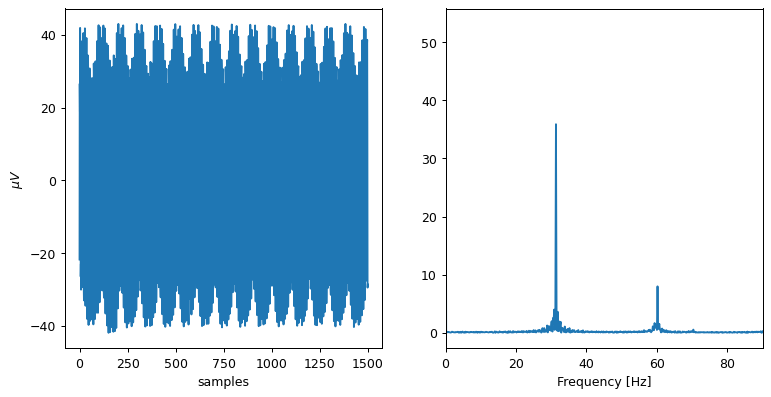
\includegraphics[width=0.8\textwidth]{Cap2/Figures/imedances_signal.png}
\par\end{centering}
\caption{Raw signal for the \textit{lead-off} configuration.}
\label{fig:bci_drivers}
\end{figure}

\begin{python}
band_2737 = GenericButterBand(27, 37, fs=250)
data = band_2737(data_raw)
\end{python}

\begin{figure}
\begin{centering}
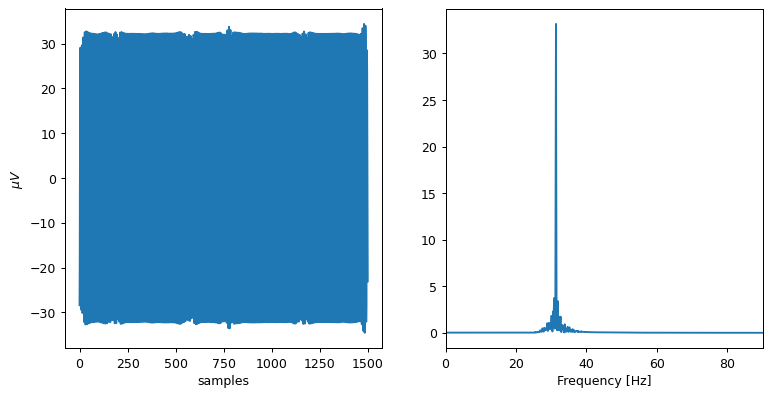
\includegraphics[width=0.8\textwidth]{Cap2/Figures/imedances_signal_filtered.png}
\par\end{centering}
\caption{Filtered signal for the \textit{lead-off} configuration.}
\label{fig:bci_drivers}
\end{figure}

The $V_{RMS}$ can be calculated as the \quot{std()} of the voltage array.

\[
V_{RMS}=\frac{V_{pp}}{2\sqrt{2}}\thickapprox std(V) 
\]

This is how our $I_{RMS}$ can be calculated:

\[
I_{RMS}=\frac{6nA}{\sqrt{2}}
\]


Then the impedance $Z$ is...

\[
Z=\frac{V_{RMS}}{I_{RMS}}
\]

Since the $V_{RMS}$ and the $std(V)$ are by default in $\mu V$, this would be the impedance measured for a vector of data $V$:

\[
Z=\frac{std(V)\cdot10^{-6}\cdot\sqrt{2}}{6\cdot10^{-9}}\:\Omega
\]

The Cyton board has a 2.2K Ohm resistors in series with each electrode, so we must remove this value in way to get the real electrode-to-head impedance.


%----------------------------------------------------------------------
\subsubsection{Real time measurement}
For this experiment we will use the Kafka consumer interface, and the same potentiometer. Keep in mind that this measurement uses one second signal, so, the variance will affect the real measure, in real-life the amplitude not change so drastically.

\begin{python}
from openbci_stream.acquisition import OpenBCIConsumer
from openbci_stream.acquisition.cyton_base import CytonConstants as cons
from openbci_stream.utils.filters import GenericButterBand
import numpy as np
import time

def get_rms(v):
    return np.std(v)

def get_z(v):
    rms = get_rms(v)
    z = (1e-6 * rms * np.sqrt(2) / 6e-9) - 2200
    if z < 0:
        return 0
    return z

Z = []
band_2737 = GenericButterBand(27, 37, fs=250)
with OpenBCIConsumer(
    'wifi',
    '192.168.1.113',
    host='192.168.1.1',
    auto_start=False,
    streaming_package_size=250,
    daisy=False,
) as (stream, openbci):
    # with OpenBCIConsumer(host='192.168.1.1') as stream:

    openbci.command(cons.SAMPLE_RATE_250SPS)
    openbci.command(cons.DEFAULT_CHANNELS_SETTINGS)
    openbci.leadoff_impedance(
        range(1, 9),
        pchan=cons.TEST_SIGNAL_NOT_APPLIED,
        nchan=cons.TEST_SIGNAL_APPLIED,
    )
    time.sleep(1)
    openbci.start_stream()

    for i, message in enumerate(stream):
        if message.topic == 'eeg':
            eeg, aux = message.value['data']
            eeg = band_2737(eeg)
            z = get_z(eeg[0])
            Z.append(z)
            print(f'{z/1000:.2f} kOhm')

        if i >= 15:
            break
\end{python}
\begin{figure}
\begin{centering}
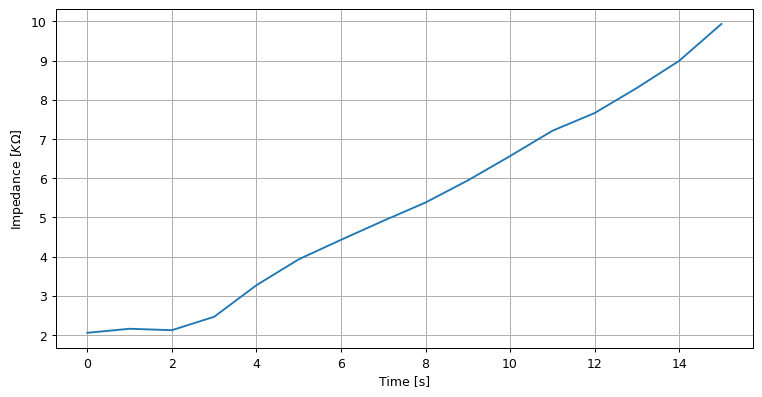
\includegraphics[width=0.8\textwidth]{Cap2/Figures/imedances_signal_pot.png}
\par\end{centering}
\caption{Real-time impedance measurement of a 10 KOhm potentiometer.}
\label{fig:bci_drivers}
\end{figure}

This measure needs a block of data to obtain a stable value. Although the method used to calculate the $V_{RMS}$ is fast, the \quot{std()}, at non-stationary times, such as while the electrode is fixed or manipulated, will affect the impedance measurement, so the calculated value will not be accurate. The measure impedance protocol requires rest periods before interpreting the value calculated.

Some recommendations for improving the impedance measurement can be:
(i) Take shorts signals but enough, 1 second is fine. 
(ii) Remove the first and last segments of the filtered signal.
(iii) Nonstationary signals will produce wrong measurements.
(iv) A single measurement is not enough, is recommended to work with trends instead.

%======================================================================
\section{Latency analysis} 

The latency comprise the time elapsed between the acquisition of raw EEG data from the OpenBCI board and the availability in the development framework. This analysis was performed over a complete distributed system and the following conditions: (i) The OpenBCI acquisition system was isolated in a dedicated Raspberry Pi, (ii) The data was read in a remote computer using the developed drivers, (iii) The block size was fixed in 100 samples, and (iv) The samples per second was fixed in 1000. The system was designed in a way that all times are registered and streamed alongside the main EEG data. This feature able to developers to perform a latency analysis without configure a special mode, this means that use the same conditions of a EEG acquisition session. 


\begin{figure}
\begin{centering}
% \includesvg[width=0.8\textwidth]{Cap4/Figures/transformer.svg}
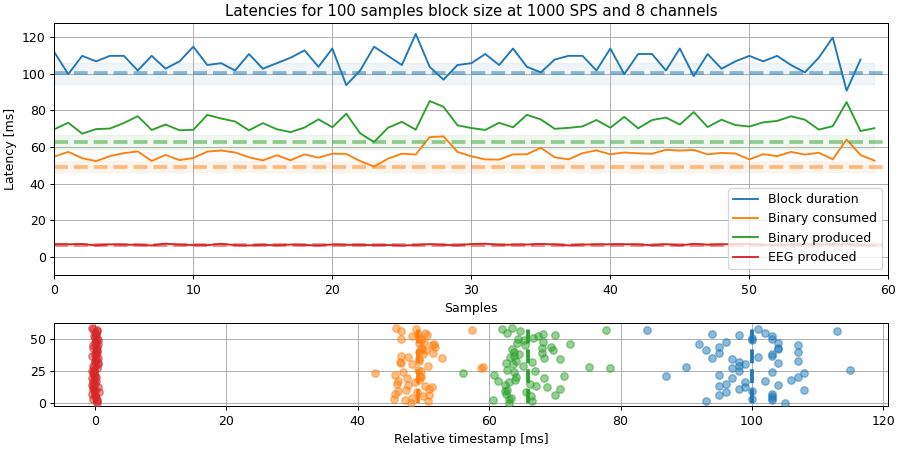
\includegraphics[width=1\textwidth]{Cap3/Figures/100ms1000sps_latencies.png}
\par\end{centering}
\caption[Latencies for 100 samples block size and 1000 SPS.]{Latencies for 100 samples block size and 1000 SPS. The latencies show the elapsed time from reading the packet to the time of packaging. The dashed line mark the minimum latency and the shade is the standard deviation for all segment.}
\label{fig:latencies_100ms}
\end{figure}

In figure \ref{fig:latencies_100ms} are plotted four relative timestamps and compared with the block duration. The \textit{Binary produced} is the time elapsed since the raw data was acquired and streamed through Kafka, \textit{Binary consumed} is the time elapsed since the binary data was consumed, just before to the deserialization, \textit{EEG produced} refers to the duration of the transmission, this is the time since the thee EEG was inserted in the Kafka stream and read in the final consumer.
There is a few facts about this plot that needs to be mentioned, 
The difference between zero and \textit{EEG produced} also includes the clock offset. 
The time bewteen \textit{Binary consumed} and \textit{EEG produced} is the time spent on the deserialization of the raw data.
The time bewteen \textit{Binary produced} and \textit{Block duration} is the time spent on the acquisition of the EEG data, this is the latency acquisition of OpenBCI when its works over the WiFi protocole. 
We can conclude then, that the deserialization process is highly time expensive.

\begin{figure}
\begin{centering}
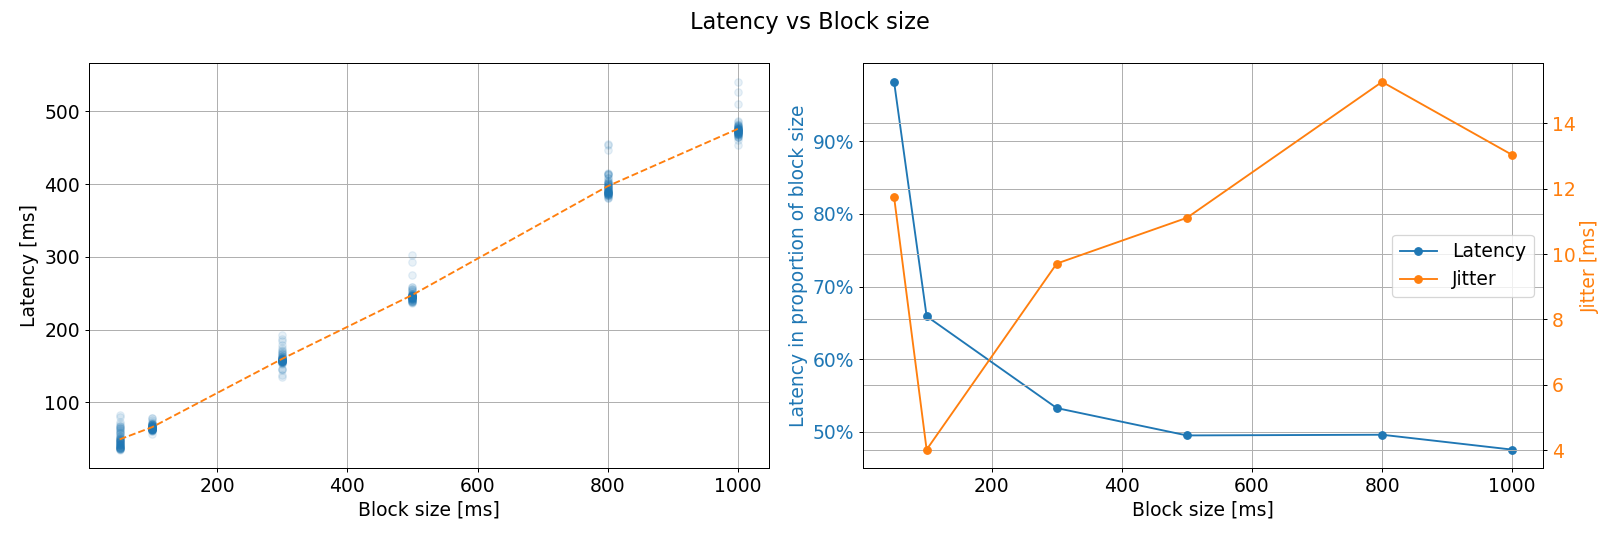
\includegraphics[width=1\textwidth]{Cap3/Figures/block_vs_latency.png}
\par\end{centering}
\caption[Latency vs Block size]{Latency vs Block size. 
In the left is possible to see that the latency is proportional to the block size. 
In the right plot, the latency decrease for small block size but their standard deviation (jitter) increase. 
The preferred configuration was set up in 100 samples block size due the lower jitter.}
\label{fig:latency_vs_block}
\end{figure}

The same process was performed for six different block sizes keeping the same 1000 SPS, the results are showed in Figure \ref{fig:latency_vs_block}, only the \textit{Binary produced} is compared with the \textit{Block size}. For block sizes under the 1000 samples and up to 100 the latency seems to be lineal.
If the data is represented using the percentage as a comparison measure, the latency seems to stabilize in $50 \%$, however the jitter appear to increase with block size. This results suggest that the optimal configuration for the EEG acquisition, using the developed drivers, is around 100 samples block size with only 8 ms of jitter.

% Preview source code for paragraph 13

\begin{table}
\begin{centering}
\begin{tabular}{>{\raggedright}p{3.3cm}cccccc}
\toprule 
\addlinespace[1em]
\textbf{BCI system} & \textbf{Sample rate} & \textbf{Block size} & \textbf{Jitter} & \textbf{Communication} & \textbf{Distributed} & \textbf{Latency}\tabularnewline\addlinespace[1em]
\midrule
\addlinespace[1em]
\textbf{BCI2000 + DT3003 \cite{schalk2004bci2000}} & 160 Hz & 6.35 ms & 0.67 ms & Wired & No & \textbf{51.9 \%}\tabularnewline
\addlinespace[0.5cm]
\textbf{BCI2000 + NI 6024E \cite{schalk2004bci2000}} & 25 kHz & 40 ms & 0.75 ms & Wired & No & \textbf{27.5 \%}\tabularnewline
\addlinespace[0.5cm]
\textbf{BCI2000 + g.USBamp \cite{wilson2010procedure}} & 1200 Hz & 83.3 ms & 5.91 ms & Wired & No & \textbf{14, 30, 48 \%}\tabularnewline
\addlinespace[0.5cm]
\textbf{OpenViBE + TMSi Porti32 \cite{kisakye2013brain}} & 512 Hz & 62.5 ms & 3.07 ms & Optical MUX & No & \textbf{100.4 \%}\tabularnewline
\addlinespace[0.5cm]
\textbf{BCI-Framework} & \textbf{1000 Hz} & \textbf{100 ms} & \textbf{5.7 ms} & \textbf{Wireless} & \textbf{Yes} & \textbf{56 \%}\tabularnewline\addlinespace[1em]
\bottomrule
\addlinespace[0.5cm]
\end{tabular}
\par\end{centering}
\caption{Latencies comparison, the latency has been expressed in terms of percentage of the block size to make the possible the comparison between different systems configurations.\label{table:latencies-comparison}}
\end{table}




Table \ref{table:latencies-comparison} show a comparison between different BCI systems configurations. The wired systems has significantly lower jitter than wireless. For centralized implementations like \textit{BCI2000 + g.USBamp} the latency depends also of the paradigm, then, the same configuration have different latencies responses.






%======================================================================
\section{Sampling analysis} 

The sampling is the process to acquire data at fixed sample rate, the acquisition process must gather the a uniform sampling rate of the signal. It is inevitable to lose data, there are some reasons, like lags in the Wi-Fi connection, in the acquisition board or in the operating system. If it is assumed that the acquisition is homogeneous, then, after a session of EEG all data will be widen to cover the supposed duration of the experiment. This will drive to an incorrect partitioning of trials. OpenBCI includes a set of special features that can be used to detect this anomalies. The first one is to use the sample indexes to detect when a data is not transmitted, and the second consist of to use known test signal. Additional to this ones, the developed drivers include a timestamp annotation for each sample that can be used too.


\begin{figure}
\begin{centering}
% \includesvg[width=0.8\textwidth]{Cap4/Figures/transformer.svg}
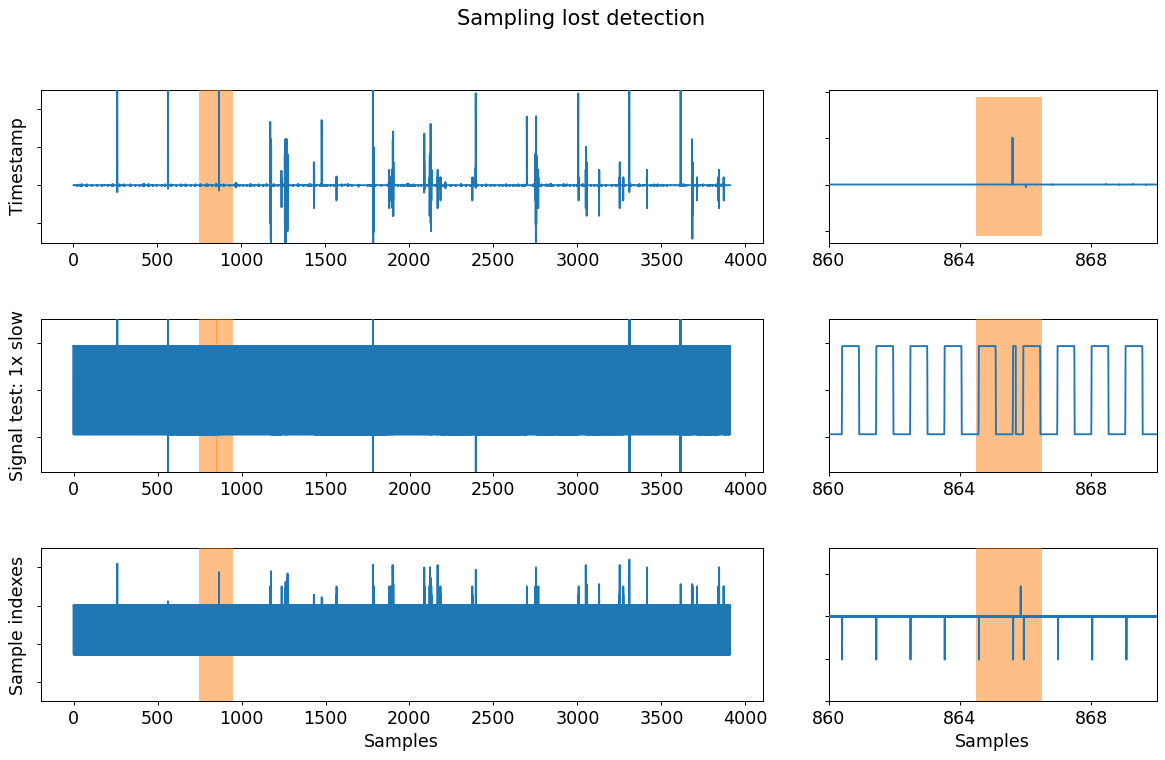
\includegraphics[width=1\textwidth]{Cap3/Figures/sampling_lost_detection.png}
\par\end{centering}
\caption[Sampling lost detection]{The sampling lost can be detected by analysing the timestamp, using a test signal or analysing the sample index.}
\label{fig:sampling_lost_detection}
\end{figure}

For the following analysis, a signal of continuous 64 minutes of acquisition was processed, recorded at 250 SPS, with 100 samples per block size and 16 channels. In Figure \ref{fig:sampling_lost_detection} are compared the three features to detect the samples skips. Any of this methods can be used to locate this points. The selected one is to use the sample indexes, this method has the advantage that can be used with a normal acquisition of EEG, the timestamp also can be used, but is more easy and fast to process the sample indexes. The test signal requires to use the channels for EEG, which makes it less practical.


\begin{figure}
\begin{centering}
% \includesvg[width=0.8\textwidth]{Cap4/Figures/transformer.svg}
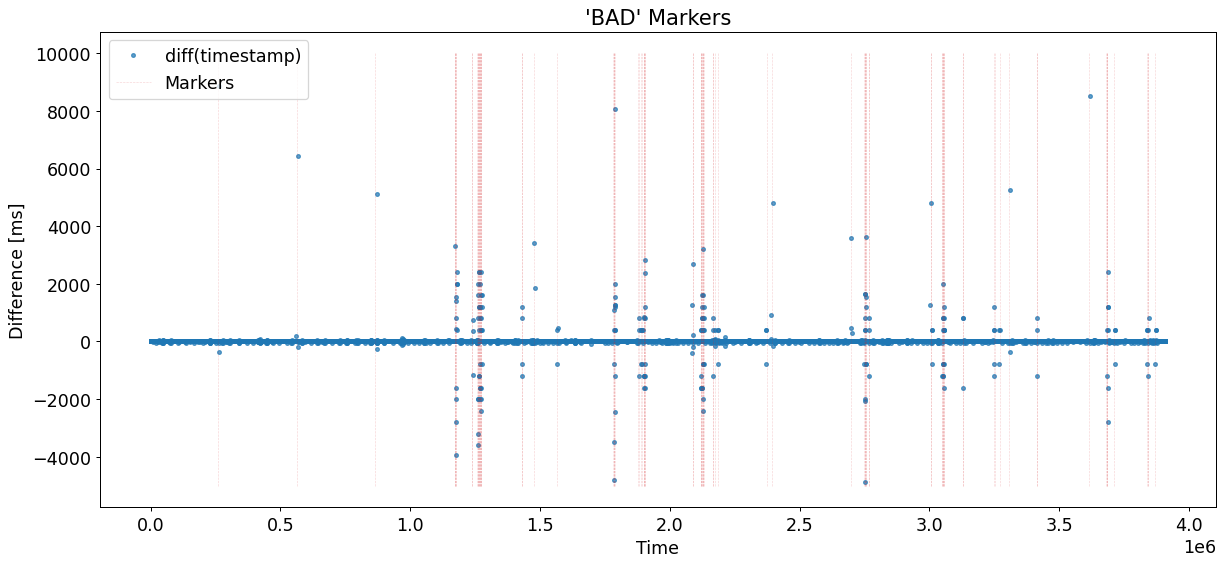
\includegraphics[width=1\textwidth]{Cap3/Figures/bad_markers_autodetection.png}
\par\end{centering}
\caption[Bad markers detection]{The bad markers detection can localize the sampling lost and place markers in that locations.}
\label{fig:bad_markers_autodetection}
\end{figure}

After to perform an algorithm to detect the sampling skips in the signals, this ones are marked as \quot{BAD:sample}. The Figure \ref{fig:bad_markers_autodetection} relates the timestamp with this markers. The \quot{BAD:sample} markers can be used to crop and remove the signal around this ones and to keep with the correctly sampling data. 


\begin{figure}
\begin{centering}
% \includesvg[width=0.8\textwidth]{Cap4/Figures/transformer.svg}
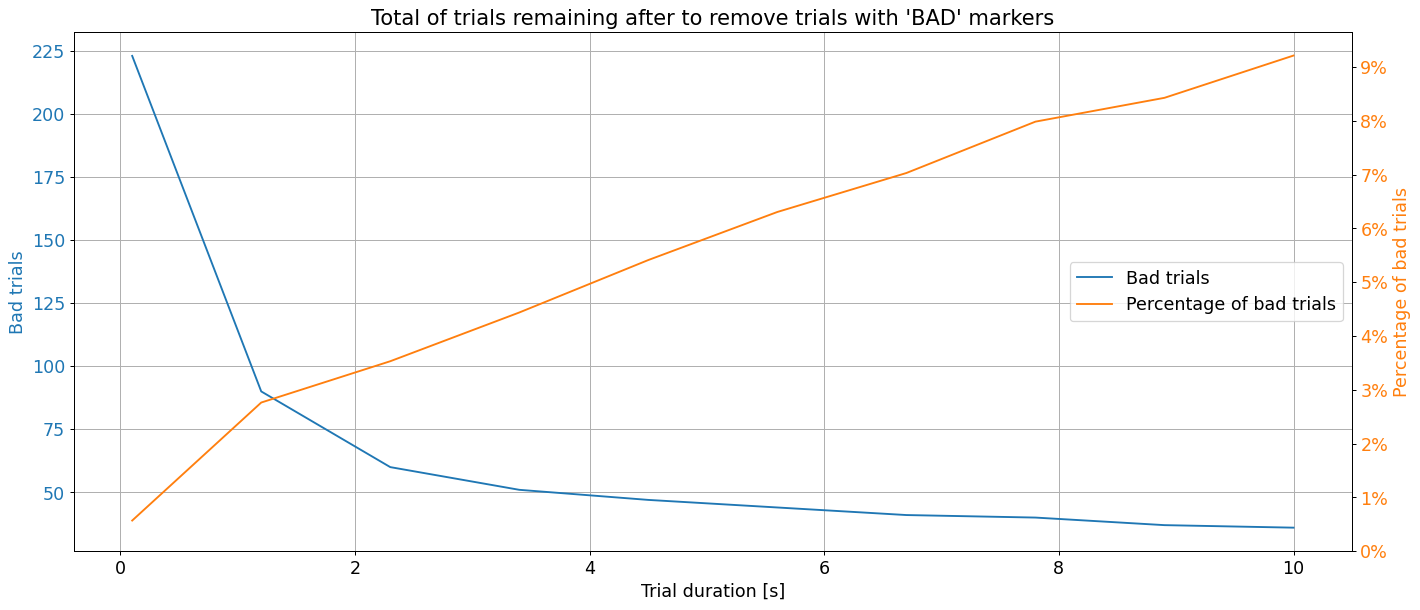
\includegraphics[width=1\textwidth]{Cap3/Figures/trials_remaning.png}
\par\end{centering}
\caption[Trials remaining after to remove trials with 'BAD' markers]{This plot show the trials and the proportion trials remaining after to remove the trials that contain almost one 'BAD' marker for a session of 60 minutes of EEG acquisition, and with a dynamical trial duration between 100 ms to 10000 ms}
\label{fig:trials_remaning}
\end{figure}

In a real experiment is desired a set of trials free of \quot{BAD} markers. The density of this markers can affect a number determined of trials depending of the size of the trial. Figure \ref{fig:trials_remaning} show the results of an experiment of 60 minutes of duration and how many trials must be discarded for each trial duration.

Figure \ref{fig:sampling_rate_analysis} compare the sampling rate around this markers. In the left without remove the skipping points, and in the right after to remove the points identified as bad samples. The right column data are more easy to interpret, the superior plot show the difference of the period in milliseconds, a solid line mark the expected $4 ms$ ($1/250 Hz$), a secondary line $50 ms$ equally distributed above and below. The inferior plot describe the mean of the period for each one of the segments resulting after removing the samples around the \quot{BAD:sample}.


\begin{figure}
\begin{centering}
% \includesvg[width=0.8\textwidth]{Cap4/Figures/transformer.svg}
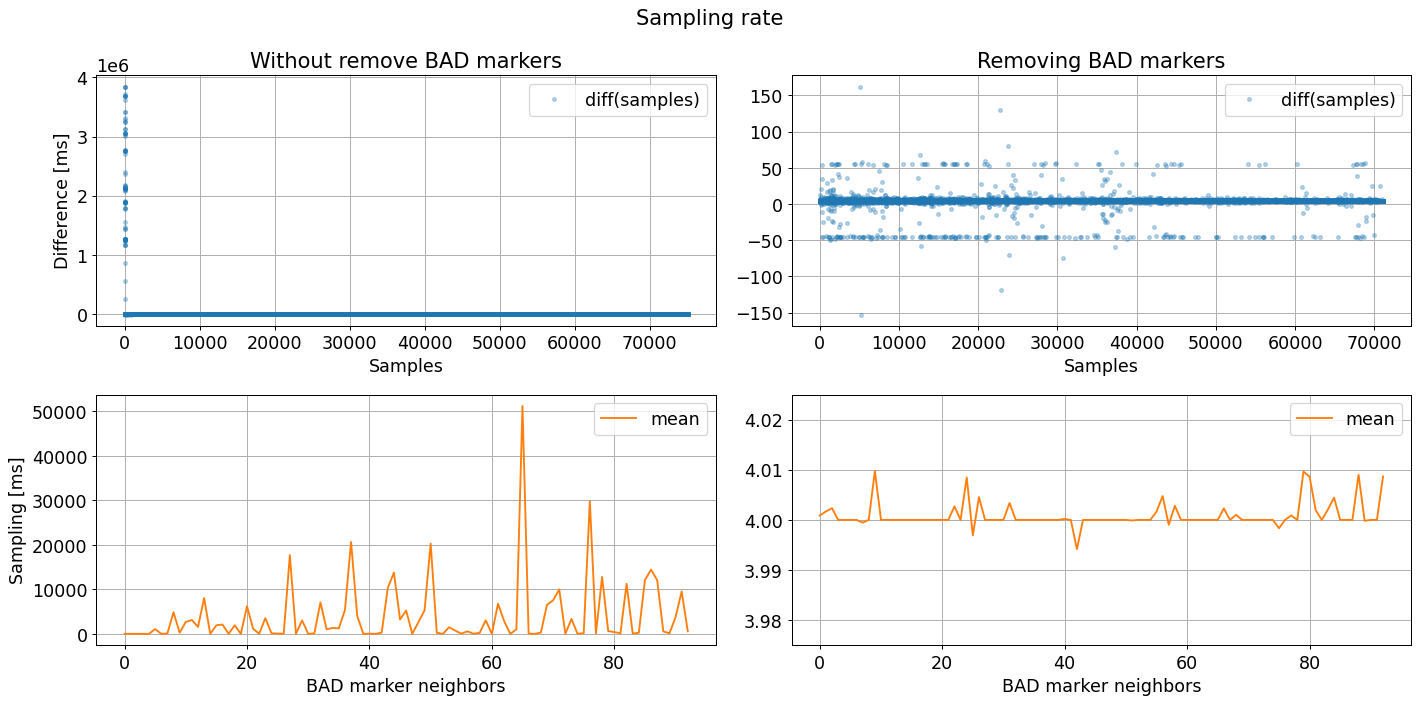
\includegraphics[width=1\textwidth]{Cap3/Figures/sampling_rate_analysis.png}
\par\end{centering}
\caption[Sampling rate analysis after remove bad markers.]{The sampling rate analysis after remove bad markers evidence a data period acquisition close to 4 ms (250 SPS).}
\label{fig:sampling_rate_analysis}
\end{figure}

%======================================================================
\section{Summary and discussion}

The real-time implementation used in this works has been fixed to guarantee the distributions of packages in a time inferior to the package duration itself. Also, the latency measures are expressed in terms of proportion of the acquisition block size, this approach facilitate the comparison with other systems and with the proposed system itself due the different acquisition configuration.

There are two resources used to implement distributed features, the first one is \gls*{RPyC}, this Python module create a remote proxy to access to the drivers module configuration and basic variables. This method use a protocol communication that is too slow to be used to stream EEG in real-time, then Kafka handles this task by implementing a real-time distributed streaming platform. Kafka, also brings other features to generate custom data streams.

The best configuration that integrate, for high sampling rate (1 KSPS), a low and stable latency was the one with fixed transmission block size of 100 samples. This configuration keeps the system stable enough to recover after interruptions and still flexible to implement real-time tasks.

Detect interruptions in the acquired signal is important for the BCI implementations, the performance of the developed systems reside on the quality of the data with which they are fed. Our drivers was designed with the feature to keep and store the data necessary to make this detection and perform automatic purge of bad trials.. 

    \chapter{BCI-Framework}\label{ch:chapter_4}

In computer programming, a framework is an abstraction in which software, providing generic functionality, can be selectively changed by additional user-written code, thus providing application-specific software. It supply a standard way to build and deploy applications and is a universal, reusable software environment that allow particular functionality as part of a larger software platform to facilitate the development of software applications, products and solutions. Frameworks-based software may include support programs, compilers, code libraries, toolsets, and application programming interfaces (\gls*{API}s) that bring together all the different components to carry up the development of a project or system \cite{soni2017full} without the need to looks out of the framework.

This chapter describe the implementation of a independent \gls*{BCI} software that consists of a distributed processing tool, stimuli delivery, psychophysiological experiments designer and real-time data visualizations for \textit{OpenBCI}. 

We purpose an open-source tool for the acquisition of EEG/EMG/ECG signals and designed to work with \textit{OpenBCI’s Cyton} board, the main core of this software lies on \footcite{OpenBCI-Stream}{https://openbci-stream.readthedocs.io} and a library designed to handle all the low-level hardware features to extend the hardware capabilities with high-level programming libraries developed in \hyperref[ch:chapter_2]{Chapter 2}. \textit{BCI-Framework} comprises a \gls*{GUI} with a set of individual computational processes (distributed or in a single machine), that feeds visualizations, serve stimuli delivery, handle acquisitions, storage data and/or process data in real-time. Additionally has a built-in development environment and a set of libraries that the user can implement to create their specific functionalities.

\textit{BCI-Framework} as well as all \gls*{BCI} applications implies the participation of at least two kind of users that will be widely used in this chapter: 
(i) the \textit{user} role refers to the person that manipulate the framework to execute experiments;
(ii) the \textit{patient} is the subject from whom the EEG data is being acquired;
(iii) a third profile can be assigned to a \textit{developer} or \textit{researcher}, this subject use the framework extensibilities to create new experiments and visualizations.


%======================================================================
\section{Software description}

BCI-Framework is a desktop application that was developed entirely using \textit{Python} and the \gls*{GUI} was implemented initially on PySide2 and updated to run under the latest stable release of \footcite{PySide6}{https://wiki.qt.io/Qt\_for\_Python}. In fact all libraries implemented are free (as in freedom) or at least \textit{Open-Source}. The software architecture is modular and designed taking into account the scalability and the configurability. Almost all components run on independent computational process and are connected to the main interface through websockets or simple \textit{HTTP} petitions.

The major feature of \textit{BCI-Framework} is the capability to implement a complete EEG-based BCI system in a single software application. This achievement, in part, is due the dedicated support to \textit{OpenBCI Cyton} board and the \hyperref[chap3:isolated-acquisition]{Isolated acquisition} that was described and implemented in Chapter 3. This feature leaves to the main machine, the one that run the framework interface, to keep all the resources to perform visualisations, processings and run a stimuli delivery server. And at the same time have a reliable flow of data.

\textit{BCI-Framework} use a set of background services that run independent of each other, some process are initialised from inside the framework and others from outside, all process run under a distributed network. All this backend services exchange information using \textit{Kafka} or \textit{Websockets}, it depends on the priority level or the amount of the information transmitted. 

% The two main backends developed with the intention to be integrated and implemented in the development of \textit{BCI-Framework} are the related with the real-time visualizations and the stimuli delivery.


%----------------------------------------------------------------------
\subsection{Real-time visualizations backend}\label{ch4:realtime_visualizations_backend}

This feature uses the \footcite{Matplotlib}{https://matplotlib.org/} backend through \footcite{FigureStream}{https://figurestream.readthedocs.io/}  a python module developed explicitly for this framework, that serve the visualization using a simple HTTP real-time streaming. This module creates a static endpoint and the image is updated like in a video streaming, this is a synchronous process, this means that the user has the control and the responsibility to feed the streaming frame by frame.

In background, a \footcite{Flask}{https://flask.palletsprojects.com/} application is running and serving the endpoint with the streaming plot for all users in the network, then, the visualizations can be both, consumed and generated from any terminal. This feature is ideal for distributed systems, since, costly real-time visualizations can be executed on a independent hardware.

The development of this backend module is described in the appendix \hyperref[appendix:matplotlib-figurestream]{Matplotlib-FigureStream}.




%----------------------------------------------------------------------
\subsection{Stimuli delivery backend}\label{ch4:stimuli_delivery_backend}

This environment is based on \textit{HTML} and \textit{JavaScript}, is basically a dynamic web application. However, in order to standardize all user scripts into a single language, this feature use \footcite{Brython}{https://brython.info/index.html}, a \textit{Python3} implementation for client-side web programming. This tool able to the user to write web applications, however, is necessary a server running with the dependencies and the library itself. With the intention to simplify the implementation and the start up of \textit{Brython} projects, a Python module called \hyperref[appendix:brython-radiant]{Brython-Radiant framework} was implemented that solve this isssues. This module is a \textit{Brython} framework for the quick development of web apps with pure \textit{Python/Brython} syntax so there is no need to care about \textit{HTML}, \textit{CSS}, or \textit{JavaScript}. Runs over \footcite{Tornado}{https://www.tornadoweb.org} and include support to \textit{Websockets}, \textit{Local Python Scripts} and \footcite{Material Design Components}{https://material.io/develop/web}. This is basically a set of scripts that allows the same script run from \textit{Python} and \textit{Brython}, when its running under \textit{Python} a \textit{Tornado} server is created and configure the local path for serving static files, and a custom \textit{HTML} template is configured in runtime to import the same script, this time, interpreted by \textit{Brython}.

\textit{Brython-Radiant} able to the user to create with pure Python and a single script a complete web application that can interact with the native Python environment. And when run under a network-based implementation allows to be consumed from any terminal. 


%======================================================================
\subsection{Development environment}

The main interface is divided into two high-level functionalities: 
(i) Real-time analysis, to collect and process data, include and interface to handle custom visualizations and serve \textit{Kafka} generators;
% (ii) Timelock analysis, to process data off-line and generate reports;
(ii) Stimuli delivery, to serve remote audiovisual stimuli and configure experiments.
This functionalities includes a set of visualizations and basic paradigms by default, instead of being rigidly included in the interface, they are in fact fully editable and configurable, even new ones can be created from scratch as an extension. All scripts are accessible under an integrated development environment.

\begin{figure}
\begin{centering}
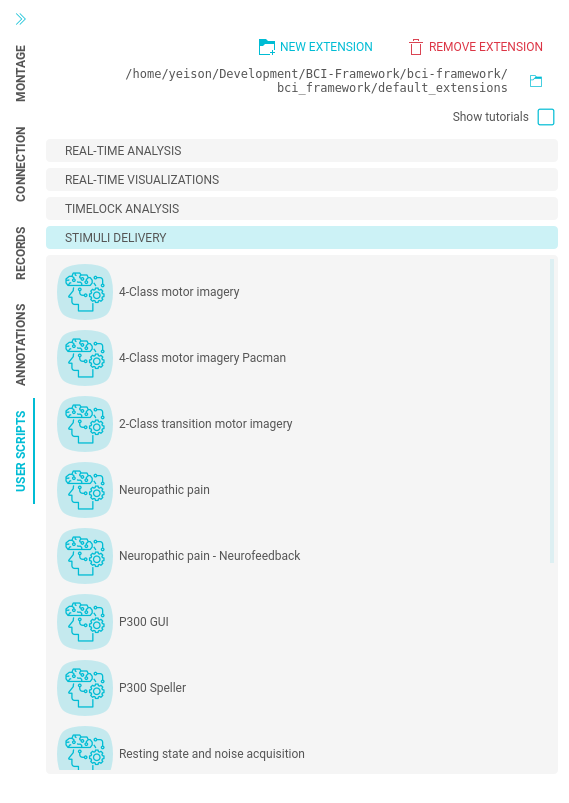
\includegraphics[width=0.5\textwidth]{Cap4/Figures/development_environment_extensions.png}
\par\end{centering}
\caption[BCI-Framework: Extensions panel]{BCI-Framework: The extensions panel is used to access to all visualizations and stimuli delivery paradigms source code, as well to create a new ones from scratch. }
\label{fig:development_environment_extension}
\end{figure}

The development environment is one of the most outstanding features of \textit{BCI-Framework}, this environment able to developers to implement custom data analysis, real-time visualizations and, design custom stimuli delivery experiments or paradigms without leaving the main interface. This is achieved by the development and the implementation of an \gls*{API} that interact with the framework parameters, the real-time data stream and with the users. Figure \ref{fig:development_environment} shows a capture of the integrated development environment, that consist of a full Python syntax highlighting, a previsualization area, a directory tree navigator, and a debugging console.




\begin{figure}
\begin{centering}
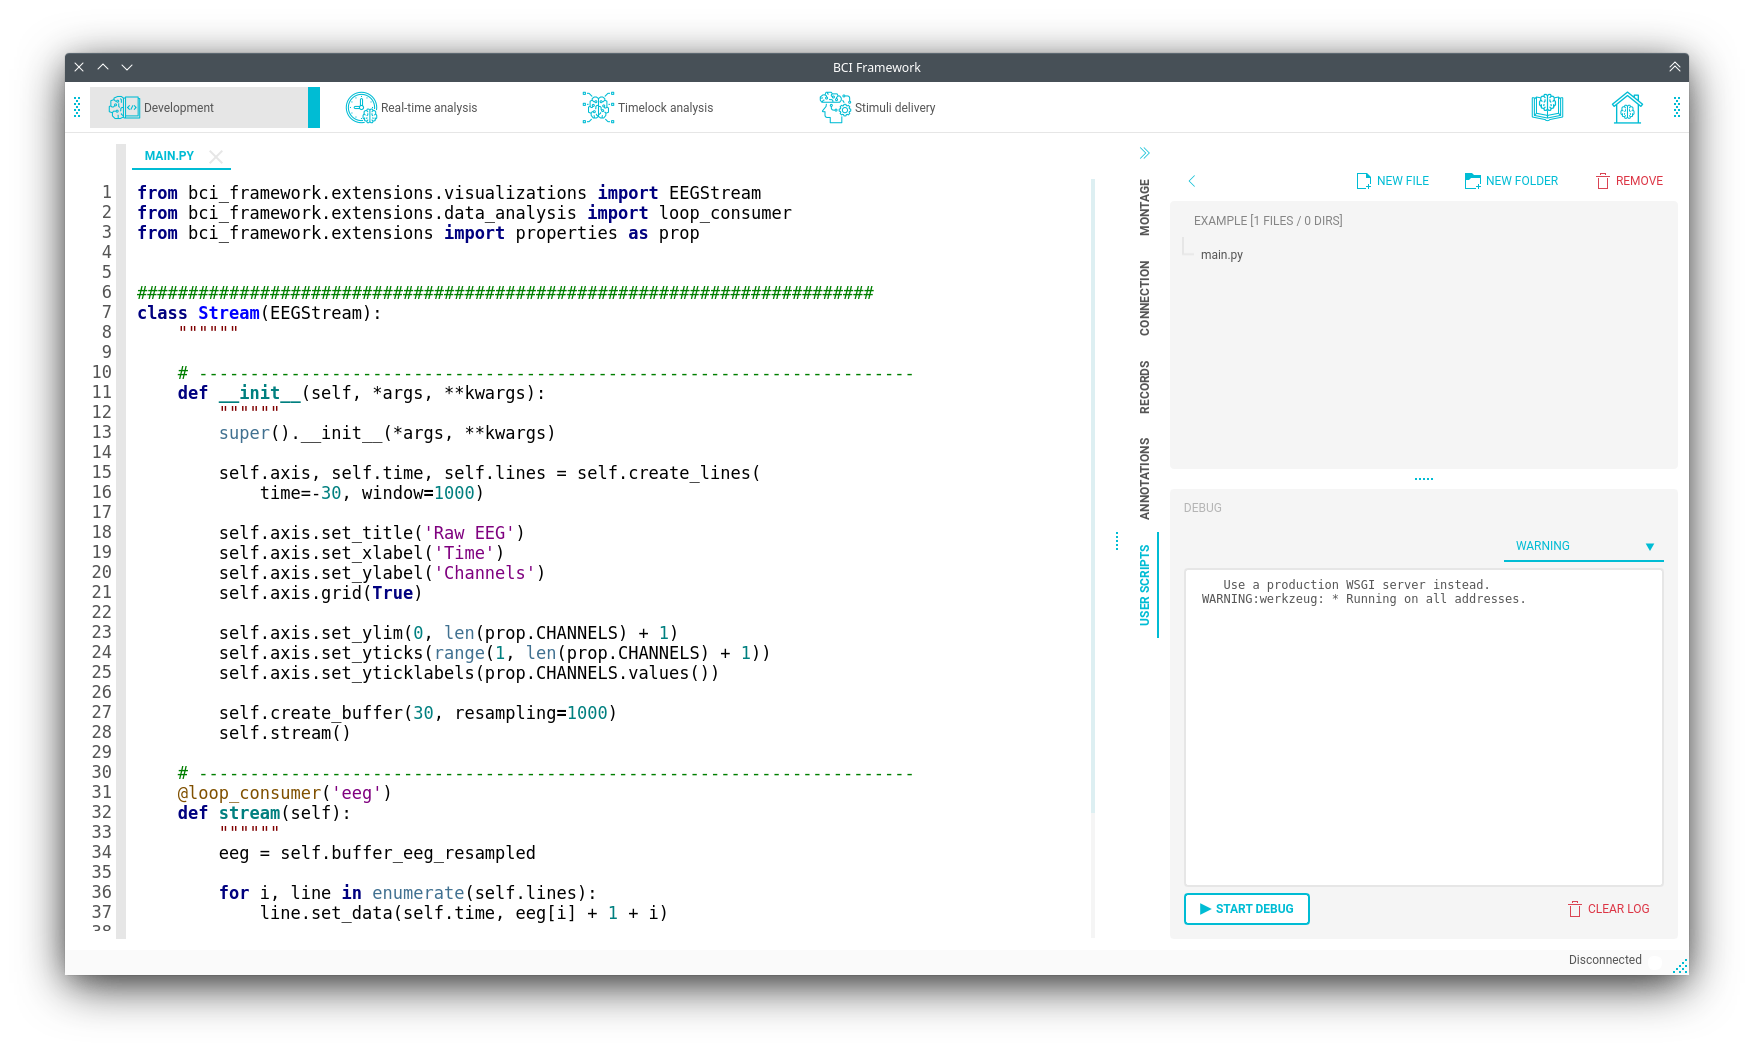
\includegraphics[width=0.8\textwidth]{Cap4/Figures/development_environment.png}
\par\end{centering}
\caption[BCI-Framework: integrated development environment]{BCI-Framework: Integrated development environment with previsualization area and debug console.}
\label{fig:development_environment}
\end{figure}



%======================================================================
\section{Real-time data analysis} \label{ch4:rt_data_analysis}  %(i.1)

The data analysis is powered by all \textit{Python} modules and the wrapped ones. This language has showed, to be a good choice for research and develop neuroscience implementations \cite{muller2015python}. Currently there are a bunch of modules like \footcite{MNE}{https://mne.tools/} specifically designed for exploring, visualizing, and analyzing human neurophysiological data. Alongside, much other that can be used to implement custom analysis like \footcite{Numpy}{https://numpy.org/} and \footcite{Scipy}{https://scipy.org/}, or for implement machine learning approaches like \footcite{Scikit-learn}{https://scikit-learn.org/} and \footcite{TensorFlow}{https://www.tensorflow.org/}.

% \textit{BCI-Framework} was designed in such a way that the user/researcher uses all this environment in combination with \gls*{EEG} signals and markers served at precise times without worry about the acquisition, synchronization and distribution. The real-time analysis is basically a \hyperref[]{Kafka consumer} or a \hyperref[]{Kafka transformer}, this component just connect with the stream that contain the \gls*{EEG} (or other signal) and consume the data to generate reports, local commands or send back a new kind of data to the stream.

\textit{BCI-Framework} was designed in such a way that the user/researcher can use the environment in combination with an easy to access \gls*{EEG} signals and markers to build their BCI system without care about the acquisition, synchronization and distribution. This approach allows to implement the real-time analysis as a basic \hyperref[]{Kafka consumer} or a \hyperref[]{Kafka transformer} that connect with the stream that contain the \gls*{EEG} (or other signal) and consume the data to serve the user/research and then generate reports, execute local commands or send back a new kind of data to the stream.

\begin{figure}
\begin{centering}
\includesvg[width=0.8\textwidth]{Cap4/Figures/kafka_transformer.svg}
\par\end{centering}
\caption[Kafka transformer]{Kafka transformer that generates a new kind of data (for example FFT) and stream it alongside the existent streams.}
\label{fig:transformer}
\end{figure}

For example, we can suppose that we need the \gls*{FFT} of the \gls*{EEG} signals in real-time, then, we can use a single script that calculate the \gls*{FFT} and create a new topic with the new data and stream it through all consumers. This transformer is graphically represented in Figure \ref{fig:transformer}, this script must run as an isolated process, and could be executed on any terminal of the network, the new data stream is automatically integrated and is available for all terminals.


%----------------------------------------------------------------------
\subsection{Data analysis scripting}\label{ch4:data_analysis}


The scripting consist of configure through a custom API the environment needed to read EEG signal. A bare minimum script looks like:

\begin{python}
from bci_framework.extensions.data_analysis import DataAnalysis

class Analysis(DataAnalysis):
    def __init__(self, *args, **kwargs):
        super().__init__(*args, **kwargs)

if __name__ == '__main__':
    Analysis()
\end{python}

The \quot{DataAnalysis} class includes a lot of useful methods to handle and configure the acquisition and manipulation of the data stream.

The API includes a custom decorator called \quot{loop\_consumer}, that is used to access asynchronously to the data stream. on every \quot{'eeg'} and \quot{'marker'} incoming data, this strings represents \textit{Kafka} topics. The \quot{stream} method only needs to be called a single time, after that, the decorator takes control of the executions, this means that entire script must finish with the call of the decorated method, in the constructor method. Is not possible, to use the decorator \quot{loop\_consumer} in more than one place, so the argument \quot{topic} could be used to create a flow control.

\begin{minted}
[
mathescape=true, 
xleftmargin=1cm, 
xrightmargin=1cm,
fontsize=\scriptsize, 
baselinestretch=1.2,
python3=true,
%  samepage=true,
% linenos=true,
highlightlines={6-10},
style=emacs,
highlightcolor=UN_primary!20,
]
{python}
from bci_framework.extensions.data_analysis import DataAnalysis, loop_consumer

class Analysis(DataAnalysis):
    def __init__(self, *args, **kwargs):
        super().__init__(*args, **kwargs)
        self.stream()

    @loop_consumer('eeg', 'marker')
    def stream(self):
        print('Incoming data...')

if __name__ == '__main__':
    Analysis()
\end{minted}

The decorated method receives five optional arguments: \quot{data}, \quot{topic}, \quot{frame}, \quot{latency} and \quot{kafka\_stream}. This arguments are defined in the wrapped decorator definition that is the reason why there is no arguments in the initial caller. This arguments works like inputs, and are optional, if some one is not declared then that local variable will be not created.

\begin{python}
@loop_consumer('eeg', 'aux')
def stream(self, data, topic, frame, latency):
    print(f'Incoming data #{frame}')
    
    match topic:
        case 'eeg':
            print(f'EEG{data.shape}')
        case 'aux':
            print(f'AUX{data.shape}')
    
    print(f'Topic: {topic}')
    print(f'Latency: {latency}')
\end{python}

\begin{python}
@loop_consumer('eeg', 'aux', 'marker')
def stream(self, topic):
    match topic:
    
        case 'eeg':
            print("EEG data incomming...")
            
        case 'aux':
            print("AUX data incomming...")

        case 'marker':
            print("Marker incomming...")
\end{python}

This scripting define the methods to subscribe to the Kafka stream topics. This solve issue about the access to the real-time data stream, however a high-level methods are also available to process, crop and buffer data.

%----------------------------------------------------------------------
\subsubsection{Buffering}

For real-time analysis, additionally to subscribe and acquire data from topics, is required a method to handle the buffer of the data acquired. The \quot{create\_buffer} method is used to configure the retention of the data streamed.

\begin{python}
self.create_buffer(seconds=30, fill=0)
\end{python}

The previous command will create a buffer of 30 seconds filled with 0 by default, the size of the buffer depends of the sampling rate and the number of the channels, this information is obtained from the framework parameters. 

\begin{minted}
[
mathescape=true, 
xleftmargin=1cm, 
xrightmargin=1cm, 
fontsize=\scriptsize, 
baselinestretch=1.2,
python3=true,
%  samepage=true,
% linenos=true,
highlightlines={4, 11-12},
style=emacs,
highlightcolor=UN_primary!20,
]
{python}
class Analysis(DataAnalysis):
    def __init__(self, *args, **kwargs):
        super().__init__(*args, **kwargs)
        self.create_buffer(seconds=30, fill=0)
        self.stream()

    @loop_consumer('eeg', 'aux')
    def stream(self):
        
        #  Buffer: all data from the last 30 seconds
        eeg = self.buffer_eeg
        aux = self.buffer_aux
         
        print(f'EEG{eeg.shape}')
        print(f'AUX{aux.shape}')
\end{minted}

Notice that the previous script has not argument in the decorated method, and that the buffer is accessible through the \quot{self.buffer\_eeg} and \quot{self.buffer\_aux} instance attributes.


%----------------------------------------------------------------------
\subsubsection{Resampling}

A sample length fixed will be created with the argument \quot{resampling}, by default is 1000 samples. A buffer for the auxiliary data with the same features is also generated. The buffering process is transparent for the user, once defined with \quot{create\_buffer} this will be automatically updated.

\begin{minted}
[
mathescape=true, 
xleftmargin=1cm, 
xrightmargin=1cm, 
fontsize=\scriptsize, 
baselinestretch=1.2,
python3=true,
%  samepage=true,
% linenos=true,
highlightlines={4, 12-13},
style=emacs,
highlightcolor=UN_primary!20,
]
{python}
class Analysis(DataAnalysis):
    def __init__(self, *args, **kwargs):
        super().__init__(*args, **kwargs)
        self.create_buffer(seconds=30, fill=0, resampling=1000)
        self.stream()

    @loop_consumer('eeg', 'aux')
    def stream(self):
        
        # Resampled buffer: 
        # the data from the last 30 seconds in a vector of 1000 samples
        eeg_r = self.buffer_eeg_resampled
        aux_r = self.buffer_aux_resampled
         
        print(f'EEG{eeg_r.shape}')
        print(f'AUX{aux_r.shape}')
\end{minted}

The resampled timeseries use the \quot{self.buffer\_eeg\_resampled} and \quot{self.buffer\_aux\_resampled} instance attributes.


%----------------------------------------------------------------------
\subsubsection{Data slicing referenced by markers}

This feature works similar to \quot{loop\_consumer}, but instead of return the latest block of data, the \quot{marker\_slicing} method return a \textit{trial}. A \textit{trial} is localized by almost one marker, and a margin time previous and posterior to the marker. 

\begin{minted}
[
mathescape=true, 
xleftmargin=1cm, 
xrightmargin=1cm, 
fontsize=\scriptsize, 
baselinestretch=1.2,
python3=true,
%  samepage=true,
% linenos=true,
highlightlines={11-12},
style=emacs,
highlightcolor=UN_primary!20,
]
{python}
from bci_framework.extensions.data_analysis import DataAnalysis, marker_slicing

class Analysis(DataAnalysis):
    def __init__(self, *args, **kwargs):
        super().__init__(*args, **kwargs)

        # Needs to be greater than the duration of the slice.
        self.create_buffer(seconds=30, aux_shape=3)
        self.slicing()

    @marker_slicing(['Right', 'Left'], t0=-2, duration=6)
    def slicing(self, eeg, aux, timestamp, marker):

        print(eeg.shape)
        print(aux.shape)
        print(timestamp.shape)
        print(marker)
        print()

if __name__ == '__main__':
    Analysis()
\end{minted}

In the previous script we are capturing trials of 6 seconds duration around the markers \quot{'Right'} and \quot{'Left'}. This feature is useful for debugging purposes, and synchronous paradigms with explicit markers presence, like \gls*{ERP}.


%----------------------------------------------------------------------
\subsubsection{Feed the stream using Kafka producer}

The data analysis can also works as a \textit{Kafka} producer, this feature is used to generate \textit{commands}, \textit{annotations}, \textit{feedbacks} and any other type of data under custom topics.

\begin{minted}
[
mathescape=true, 
xleftmargin=1cm, 
xrightmargin=1cm,
fontsize=\scriptsize, 
baselinestretch=1.2,
python3=true,
%  samepage=true,
% linenos=true,
highlightlines={8},
style=emacs,
highlightcolor=UN_primary!20,
]
{python}
from bci_framework.extensions.data_analysis import DataAnalysis

class Analysis(DataAnalysis):
    def __init__(self, *args, **kwargs):
        super().__init__(*args, **kwargs)

if __name__ == '__main__':
    Analysis(enable_produser=True)
\end{minted}

Once activate the producer, the \quot{send\_command}, \quot{send\_feedback} and \quot{send\_annotation} methods are available.

\begin{python}
# Command
self.send_command('MyCommand', value=45)

# Annotation
self.send_annotation('The subject yawn', duration=5)

# Feedback
feed = {'var1': 0,
        'var2': True,
        'var3': 'Right',
       }
self.send_feedback(**feed)

# send_feedback method are keyword arguments only
self.send_feedback(a=0, b=2.3, c='Left')

# Custom topic
self.generic_produser('my_topic', my_data)

\end{python}

The \quot{generic\_produser} method can be used to stream any custom data under a user defined topic. 
% The difference with the methods to stream \textit{commands}, \textit{annotations}, and \textit{feedbacks} resides on that the framework will interprets this lasts using specific process, and sometimes could execute instruction over the framework itself.

% %----------------------------------------------------------------------
% \subsection{Default data analysis}


%======================================================================
\section{Real-time visualization}  %(i.2)

The visualizations works very similar that the \hyperref[ch4:rt_data_analysis]{Real-time analysis}, with the difference that only comprise \hyperref[]{Kafka consumers} due the visualization is indented to be displayed inside of the \textit{BCI-Framework} interface and over a \textit{HTTP} protocol instead to create a new kind of data stream. 

\begin{figure}
\begin{centering}
\includesvg[width=0.8\textwidth]{Cap4/Figures/kafka_consumer.svg}
\par\end{centering}
\caption[kafka consumer]{Kafka consumer that access to the real-time EEG stream and use the data to perform individual process.}
\label{fig:transformer}
\end{figure}

The real-time visualizations consists of a computational process that manipulate the data in order to create static visualization and then update this one consecutively. The environment to create visualizations automatically serve the real-time EEG stream, then the user only must comply about the visualizations.


%----------------------------------------------------------------------
\subsection{Data visualization scripting}\label{ch4:viz_development}%(i.2)

Data visualization are based on \hyperref[appendix:matplotlib-figurestream]{Matplotlib-FigureStream}, this interface inherits all features from it and extends the utilities with an specific ones. Additionally all topics explained in \hyperref[ch4:data\_analysis]{Real-time analysis development} are valid here too, since visualizations is a special case of real-time analysis.

\begin{minted}
[
mathescape=true, 
xleftmargin=1cm, 
xrightmargin=1cm,
fontsize=\scriptsize, 
baselinestretch=1.2,
python3=true,
%  samepage=true,
% linenos=true,
highlightlines={4,17},
style=emacs,
highlightcolor=UN_primary!20,
]
{python}
from bci_framework.extensions.visualizations import EEGStream
from bci_framework.extensions.visualizations.utils import loop_consumer

class Stream(EEGStream):  # This is `matplotlib.Figure` based class
    def __init__(self):
        super().__init__()

        self.axis = self.add_subplot(111)
        self.axis.set_title('Title')
        self.axis.set_xlabel('Time')
        self.axis.set_ylabel('Amplitude')
        self.axis.grid(True)
        self.stream()

    @loop_consumer('eeg')
    def stream(self, *args, **kwargs):
        self.feed()

if __name__ == '__main__':
    Stream()
\end{minted}

Here the main difference is the class to heritage, \quot{EEGStream}, and the \quot{self.feed()} method. In this bare minimum example the constructor generates an empty plot using standard \textit{matplotlib} and them the \quot{loop\_consumer} will serve the data to the developer disposition.
% There is no limitations about the kind of plot that can be implemented here, only the ones related with performance.

\begin{python}
@loop_consumer('eeg')
def stream(self, data):
    eeg, aux = data

    ch0 = eeg[0]  # first eeg channel
    self.line.set_ydata(ch0)
    self.axis.set_ylim(ch0.min(), ch0.max())

    time = range(len(ch0))  # time axis
    self.line.set_xdata(time)
    self.axis.set_xlim(time[0], time[-1])

    self.feed()
\end{python}

The \quot{loop\_consumer} is used to update asynchronously the plot, since this method is executed on every new package received, this continuous update will create a plotting animation. The \quot{self.feed()} method send an update to the plotting stream server.

% %----------------------------------------------------------------------
% \subsection{Default data visualization}


%======================================================================
\section{Stimuli delivery} %(iii)

The interface for stimuli delivery is the only that interact directly with the \textit{patient}, neurophysiological experiments requires a controlled environment with the purpose to decrease the artifacts \cite{vialatte2008eeg, gomez2006automatic} in the signal as well as keep the patient concentrated on his task. This requirements suggest that the stimuli delivery must work over a remote presentation system and, in this way, separate physically the \textit{user} from the \textit{patient}. The method selected to develop an environment with these features was the classic web application based on HTML, CSS and JavasScript through the implementation of the \hyperref[appendix:brython-radiant]{Brython-Radiant framework}.

Although this is a common feature in almost all neurophysiological experiments designer software, after a series of observations and experience acquiring databases for the SPGR, we propose a brand new environment for the design, implementation and configuration of audio-visual stimuli delivery. Our interface able to the user to design flexible experiments and change the parameter easy and quickly without reprogramming the paradigm. Also, since the acquisition interface is integrated into the framework the database is generated automatically with all respective metadata and synchronized markers. Then the user only has to worry about the experiment while the database is generated in second plane.

\begin{figure}
\begin{centering}
% \includesvg[width=0.8\textwidth]{Cap4/Figures/transformer.svg}
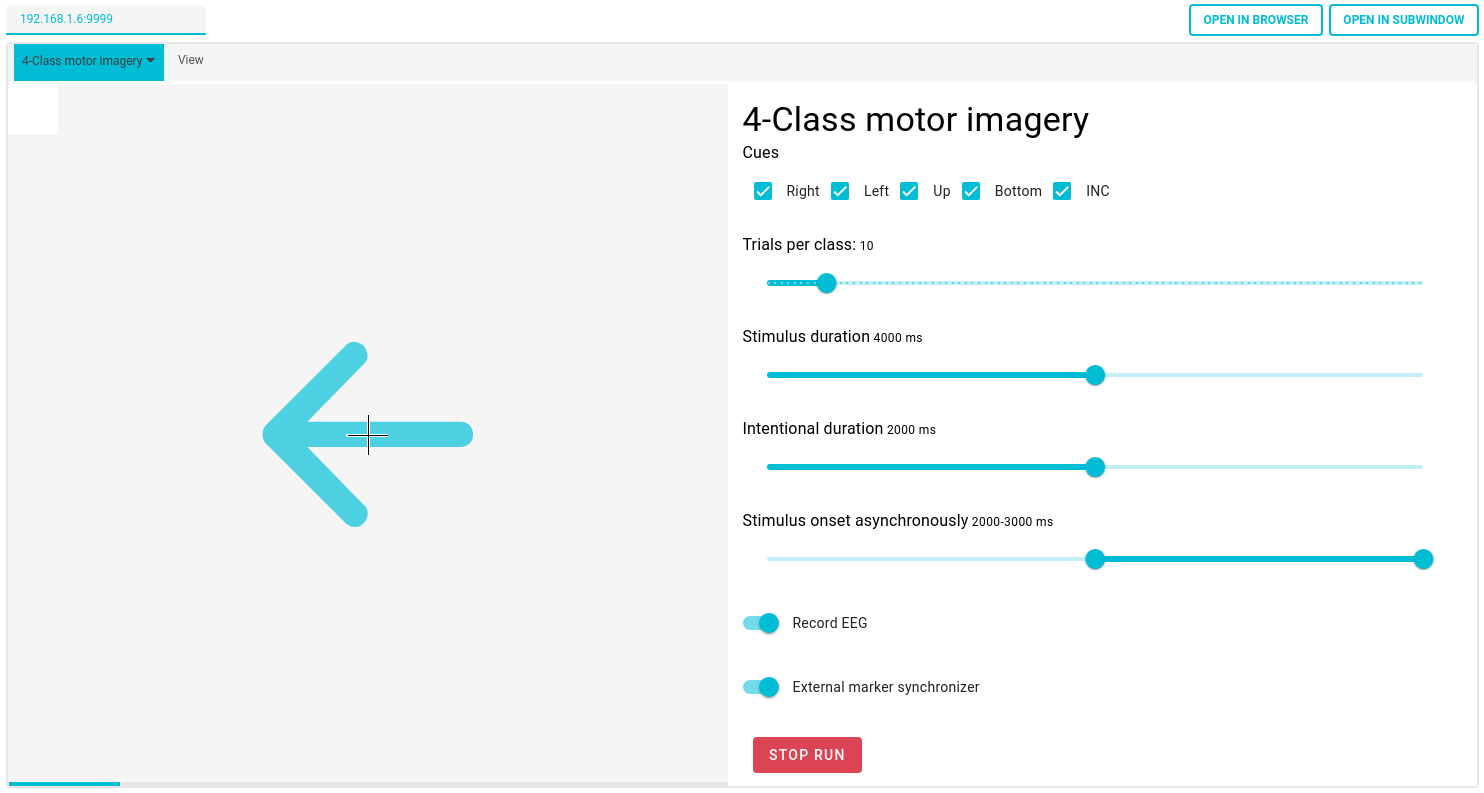
\includegraphics[width=0.8\textwidth]{Cap4/Figures/stimuli_delivery.png}
\par\end{centering}
\caption[Stimuli delivery interface]{Stimuli delivery interface, in the left the live view of the stimulus presented remotely to the patient, in the right the dashboard with the main parameter of the experiment.}
\label{fig:stimuli_delivery_interface}
\end{figure}

The proposal interface still requires that both, the stimuli delivery and the previsualization in the dashboard, update the screen synchronously. Then there are two kind of views, the first one is for the \textit{patient}, this view only includes the stimuli presentation and is the responsible to create the time markers. The second view is for the \textit{user}, additional to the stimuli preview also include a dashboard, this interface able to configure the experiment execution. 

%----------------------------------------------------------------------
\subsection{Stimuli delivery scripting}\label{ch4:stimuli_delivery_designer}%(iii)

This interface environment use \textit{Brython} and the \textit{Radiant framework} as backend for do the web development in a \textit{Python} style.

\begin{minted}
[
mathescape=true, 
xleftmargin=1cm, 
xrightmargin=1cm,
fontsize=\scriptsize, 
baselinestretch=1.2,
python3=true,
%  samepage=true,
% linenos=true,
highlightlines={3-5,12-17},
style=emacs,
highlightcolor=UN_primary!20,
]
{python}
from bci_framework.extensions.stimuli_delivery import StimuliAPI

# Brython modules
from browser import document, html
from browser.widgets.dialog import InfoDialog

class StimuliDelivery(StimuliAPI):
    def __init__(self, *args, **kwargs):
        super().__init__(*args, **kwargs)
        document.clear()

        # main brython code
        document.select_one('body') <= html.H3('Hello world')

        button = html.BUTTON('click me')
        button.bind('click', lambda evt: InfoDialog('Hello', 'world'))
        document.select_one('body') <= button

if __name__ == '__main__':
    StimuliDelivery()
\end{minted}

The \quot{StimuliAPI} includes lot of methods to simplify the interaction with the stimuli delivery environment


%----------------------------------------------------------------------
\subsubsection{Stimuli area and Dashboard}

One of the main features is the possibility to make configurable experiments, in favor to this philosophy, by default they are build both areas, \quot{self.stimuli\_area} and \quot{self.dashboard} in the class constructor.

% \begin{python}
self.stimuli_area <= html.H3('Stimuli area')
self.dashboard <= html.H3('Dashboard')

# Insert a cross in the middle of the stimuli area
self.show_cross()

# This area is used for external event processord
self.show_synchronizer()
\end{python}
% \begin{figure}
\begin{centering}
% \includesvg[width=0.8\textwidth]{Cap4/Figures/transformer.svg}
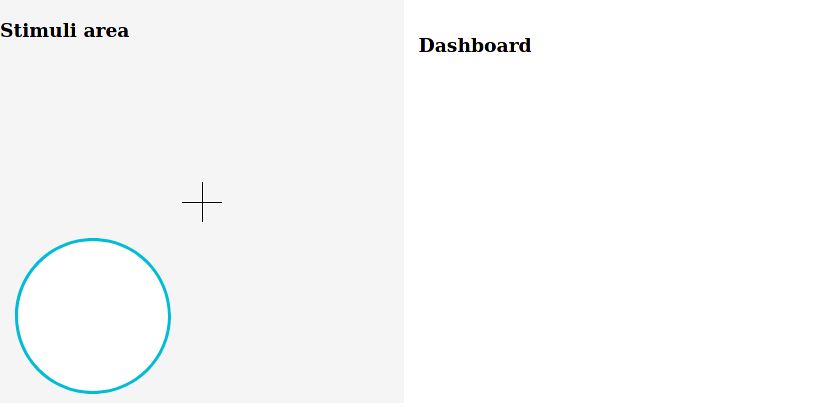
\includegraphics[width=0.8\textwidth]{Cap4/Figures/stimuli_delivery_areas.png}
\par\end{centering}
\caption[]{.}
\label{fig:stimuli_delivery_interface}
\end{figure}

The attempt use of the stimuli area is to use it to present the stimulus, this area is automatically duplicated in the remote patient view. The right side is intended to the dashboard, this layout is only accessible for the user, and is used to configure the experiment.

The both areas are accessible thought the class attribute \quot{self.stimuli\_area} and \quot{self.dashboard}, as instances of \quot{browser.html.DIV}. There is a particularity in the language about the use of \quot{<=} to nest elements.


%----------------------------------------------------------------------
\subsection{Widgets}

All widgets and styles are part of \footcite{Material Components Web}{https://material.io/develop/web} and can be implemented with a custom module implementation designed to display widgets and get values. All widgets are available troughs the \quot{Widgets} submodule located in the module \quot{bci\_framework.extensions.stimuli\_delivery.utils}.

\begin{python}
from bci_framework.extensions.stimuli_delivery.utils import Widgets as w
\end{python}

%----------------------------------------------------------------------
\subsubsection{Typography}
Not only for aesthetics, a default font was selected to make the messages easy to read, even on small screens, in combination with a set of hierarchies and contexts.
\begin{python}
self.dashboard <= w.label('headline1', typo='headline1')
self.dashboard <= w.label('headline2', typo='headline2')
self.dashboard <= w.label('headline3', typo='headline3')
self.dashboard <= w.label('headline4', typo='headline4')
self.dashboard <= w.label('headline5', typo='headline5')
self.dashboard <= w.label('headline6', typo='headline6')
self.dashboard <= w.label('body1', typo='body1')
self.dashboard <= w.label('body2', typo='body2')
self.dashboard <= w.label('subtitle1', typo='subtitle1')
self.dashboard <= w.label('subtitle2', typo='subtitle2')
self.dashboard <= w.label('caption', typo='caption')
self.dashboard <= w.label('button', typo='button')
self.dashboard <= w.label('overline', typo='overline')
\end{python}

\begin{figure}[H]
\begin{centering}
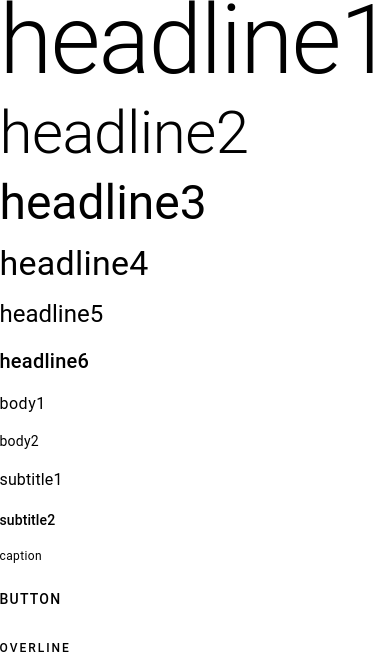
\includegraphics[scale=0.5]{Cap4/Figures/widgets/typography.png}
\par\end{centering}
\caption[Brython Radiant: Typography]{Brython Radiant: Default typography.}
\label{fig:radiant_typography}
\end{figure}

%----------------------------------------------------------------------
\subsubsection{Buttons}
The buttons have the action \quot{on\_click} associated, this action just trigger a method, a function or an anonymous function.
\begin{python}
    self.dashboard <= w.label('Buttons', typo='headline4', style=flex_title)
    self.dashboard <= w.button(
        'Button 1',
        style=flex,
        on_click=lambda: setattr(
            document.select_one('#for_button'), 'html', 'Button 1 pressed!'
        ),
    )
    self.dashboard <= w.button(
        'Button 2', style=flex, on_click=self.on_button2
    )
    self.dashboard <= w.label(
        f'', id='for_button', typo=f'body1', style=flex
    )

def on_button2(self):
    document.select_one('#for_button').html = 'Button 2 pressed!'
\end{python}


\begin{figure}[H]
\begin{centering}
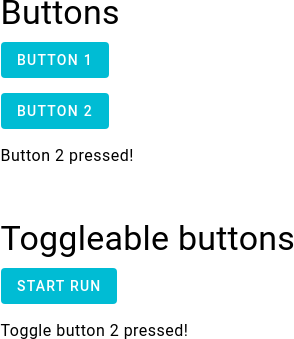
\includegraphics[scale=0.5, left]{Cap4/Figures/widgets/buttons.png}
\par\end{centering}
\caption[Brython Radiant: Buttons]{Brython Radiant: Buttons.}
\label{fig:radiant_buttons}
\end{figure}

%----------------------------------------------------------------------
\subsubsection{Switch}
The switch, like the button, have an action associated, but also, a state. The state can be getted on any moment using the \quot{id} with the method \quot{get\_value(id)} or in the argument of the binded action.
\begin{python}
    self.dashboard <= w.label('Switch', typo='headline4', style=flex_title)
    self.dashboard <= w.switch(
        'Switch 1', checked=True, on_change=self.on_switch, id='my_swicth'
    )
    self.dashboard <= w.label(
        f'', id='for_switch', typo=f'body1', style=flex
    )


def on_switch(self, value):
    # value = self.widgets.get_value('my_swicth')
    document.select_one('#for_switch').html = f'Switch Changed: {value}'
\end{python}


\begin{figure}[H]
\begin{centering}
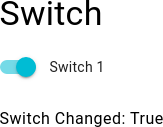
\includegraphics[scale=0.5]{Cap4/Figures/widgets/switch.png}
\par\end{centering}
\caption[Brython Radiant: Switch]{Brython Radiant: Switch.}
\label{fig:radiant_switch}
\end{figure}

%----------------------------------------------------------------------
\subsubsection{Checkbox}
Multiple selection list items use the checkbox to interact with this list of items, the state comprise the list of selected options, and \quot{on\_change} is triggered on every item status changed.
\begin{python}
    self.dashboard <= w.label('Checkbox', typo='headline4', style=flex_title)
    self.dashboard <= w.checkbox(
        'Checkbox',
        options=[[f'chb-{i}', False] for i in range(4)],
        on_change=self.on_checkbox,
        id='my_checkbox',
    )
    self.dashboard <= w.label(
        f'', id='for_checkbox', typo=f'body1', style=flex
    )


def on_checkbox(self):
    value = w.get_value('my_checkbox')
    document.select_one('#for_checkbox').html = f'Checkbox Changed: {value}'
\end{python}


\begin{figure}[H]
\begin{centering}
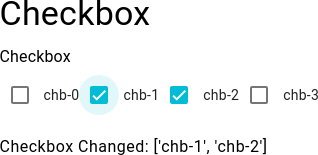
\includegraphics[scale=0.5]{Cap4/Figures/widgets/checkbox.png}
\par\end{centering}
\caption[Brython Radiant: Checkbox]{Brython Radiant: Checkbox.}
\label{fig:radiant_checkbox}
\end{figure}


%----------------------------------------------------------------------
\subsubsection{Radios}
Similar to checkboxes but, the selection is exclusive to only one item, then the state is a string.
\begin{python}
    self.dashboard <= w.label('Radios', typo='headline4', style=flex_title)
    self.dashboard <= w.radios(
        'Radios',
        options=[[f'chb-{i}', f'chb-{i}'] for i in range(4)],
        on_change=self.on_radios,
        id='my_radios',
    )
    self.dashboard <= w.label(
        f'', id='for_radios', typo=f'body1', style=flex
    )


def on_radios(self):
    value = w.get_value('my_radios')
    document.select_one('#for_radios').html = f'Radios Changed: {value}'
\end{python}


\begin{figure}[H]
\begin{centering}
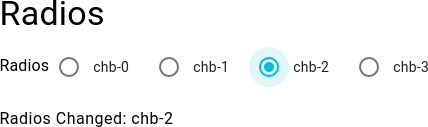
\includegraphics[scale=0.5]{Cap4/Figures/widgets/radios.png}
\par\end{centering}
\caption[Brython Radiant: Radios]{Brython Radiant: Radios.}
\label{fig:radiant_radios}
\end{figure}

%----------------------------------------------------------------------
\subsubsection{Select}
The select component comply the same function that the radios, but the interface is displayed to the user using a different widget. 
\begin{python}
    self.dashboard <= w.label('Select', typo='headline4', style=flex)
    self.dashboard <= w.select(
        'Select',
        [[f'sel-{i}', f'sel-{i}'] for i in range(4)],
        on_change=self.on_select,
        id='my_select',
    )
    self.dashboard <= w.label(
        f'', id='for_select', typo=f'body1', style=flex
    )


def on_select(self, value):
    # value = w.get_value('my_select')
    document.select_one('#for_select').html = f'Select Changed: {value}'
\end{python}


\begin{figure}[H]
\begin{centering}
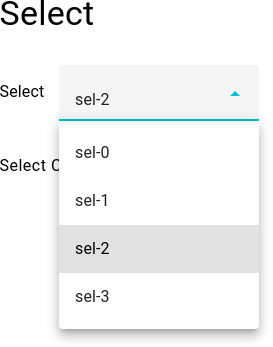
\includegraphics[scale=0.5]{Cap4/Figures/widgets/select.png}
\par\end{centering}
\caption[Brython Radiant: Select]{Brython Radiant: Select.}
\label{fig:radiant_select}
\end{figure}


%----------------------------------------------------------------------
\subsubsection{Sliders}
The slider are used to select numbers from a range or a range itself. The state is the value or the range and the trigger event is the continuous update, not the change after a release.
\begin{python}
    # Slider
    self.dashboard <= w.label('Slider', typo='headline4', style=flex)
    self.dashboard <= w.slider(
        'Slider',
        min=1,
        max=10,
        step=0.1,
        value=5,
        on_change=self.on_slider,
        id='my_slider',
    )
    self.dashboard <= w.label(
        f'', id='for_slider', typo=f'body1', style=flex
    )

    # Slider range
    self.dashboard <= w.label('Slider range', typo='headline4', style=flex)
    self.dashboard <= w.range_slider(
        'Slider range',
        min=0,
        max=20,
        value_lower=5,
        value_upper=15,
        step=1,
        on_change=self.on_slider_range,
        id='my_range',
    )
    self.dashboard <= w.label(f'', id='for_range', typo=f'body1', style=flex)


def on_slider(self, value):
    # value = w.get_value('my_slider')
    document.select_one('#for_slider').html = f'Slider Changed: {value}'


def on_slider_range(self, value):
    # value = w.get_value('my_slider')
    document.select_one('#for_range').html = f'Range Changed: {value}'
\end{python}


\begin{figure}[H]
\begin{centering}
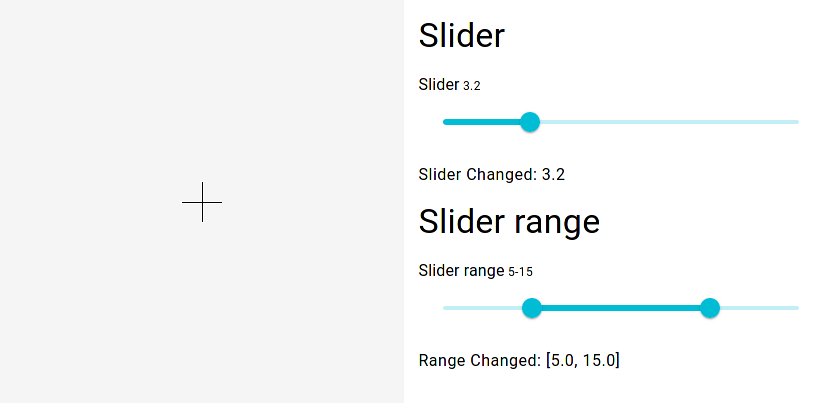
\includegraphics[scale=0.5]{Cap4/Figures/widgets/sliders.png}
\par\end{centering}
\caption[Brython Radiant: Slider]{Brython Radiant: Sliders.}
\label{fig:radiant_sliders}
\end{figure}

%----------------------------------------------------------------------
\subsection{Audiovisual stimuli}

Since Brython-Radiant is basically a frontend framework, all visual stimuli can be implemented through JavaScript, HTML, and CSS. Web applications are the most featured environ to develop audivisual stimuli. Present and update views, reproduce audio or video are basic tasks in this environment. 

%----------------------------------------------------------------------
\subsubsection{Tones and audio}

The \textit{Tone} library allows playing single notes using the \quot{javascript} \quot{AudioContext backend}, the duration and the gain can also be configured.
\begin{python}
from bci_framework.extensions.stimuli_delivery.utils import Tone as t

duration = 100
gain = 0.5

self.dashboard <= w.button(
    'f#4',
    on_click=lambda: t('f#4', duration, gain),
    style={'margin': '0 15px'},
)
self.dashboard <= w.button(
    'D#0',
    on_click=lambda: t('D#0', duration, gain),
    style={'margin': '0 15px'},
)
self.dashboard <= w.button(
    'B2',
    on_click=lambda: t('B2', duration, gain),
    style={'margin': '0 15px'},
)
\end{python}

The Audio module allows to reproduce complete audio files.
\begin{python}
from bci_framework.extensions.stimuli_delivery.utils import Audio as a

a.load('rain.wav')

self.dashboard <= w.label(
    'Audio',
    'headline4',
    style={
        'margin-bottom': '15px',
        'display': 'flex',
    },
)
self.dashboard <= html.BR()

self.dashboard <= w.slider(
    'Gain',
    min=0,
    max=1,
    step=0.1,
    value=0.5,
    id='gain',
    on_change=a.set_gain,
)

self.dashboard <= w.button(
    'Start', on_click=a.play, style={'margin': '0 15px'}
)
self.dashboard <= w.button(
    'Stop', on_click=a.stop, style={'margin': '0 15px'}
)

\end{python}

%----------------------------------------------------------------------
\subsubsection{Visual stimuli}

A complete free HTML-based environment available to design and implement neurophysiological experiments.

\begin{python}
from bci_framework.extensions.stimuli_delivery.utils import icons

self.dashboard <= icons.fa('fa-arrow-right')   # FontAwesome
self.dashboard  <= icons.bi('bi-arrow-right')  # Bootstrap icon
self.dashboard  <= icons.mi('face', size=24)   # Material icons 
\end{python}

%----------------------------------------------------------------------
\subsection{Stimuli delivery pipeline}

Pipelines consist of the controlled execution of methods with asynchronous timeouts. We define a paradigm as a sequence of trials, and each trial is composed of a sequence of parameterized views. 

For example, in the classic motor imagery paradigm with two classes, right and left. A trial is the presentation of one stimulus, each trial is composed of a sequence of views: clear screen, wait, show stimulus, clear screen. And then, the next trial with the same sequence of views but with different parameters, like the stimulus itself, or random waits.

This task can be implemented programmatically with the pipeline design pattern and simplified the implementation. First one we need to define the trials like a list of  parameter used for each one of the single trial. For example, here we define 3 trials:

\begin{python}
trials = [
    {'s1': 'Left',  # Trial 1
     'r1': 91,
     },

    {'s1': 'Right',  # Trial 2
     'r1': 85,
     },

    {'s1': 'Left',  # Trial 3
     'r1': 30,
     },
]
\end{python}

And the trial views consists of a list of sequential methods with a respective timeout (method, timeout), if the timeout is a number then this will indicate the milliseconds until the next method call. If the timeout is a list, then a random (with uniform distribution) number between that range will be generated on each trial.

\begin{python}
view = [
    (self.view1, 500),
    (self.view2, [500, 1500]),
    (self.view3, w.get_value('slider')),
    (self.view4, w.get_value('range')),
]
\end{python}

The view configuration can used states from widgets by referencing the \quot{id} instead of an explicit value:

\begin{python}
view = [
    (self.view1, 500),          # timeout
    (self.view2, [500, 1500]),  # range
    (self.view3, 'slider'),     # from widgets id
    (self.view4, 'range'),
]
\end{python}

Then, we need to define the views methods, each method  is a step needed to build a single trial. By definition, all views will share the same arguments, even if they are not used by that method.
 
\begin{python}
def view1(self, s1, r1):
    print(f'On view1: {s1=}, {r1=}')

def view2(self, s1, r1):
    print(f'On view2: {s1=}, {r1=}')

def view3(self, s1, r1):
    print(f'On view3: {s1=}, {r1=}')

def view4(self, s1, r1):
    print(f'On view4: {s1=}, {r1=}\n')
\end{python}

Finally, our pipeline can be executed with the method \quot{self.run\_pipeline}:

\begin{python}
self.run_pipeline(view, trials)
\end{python}

Here, the pipeline is running all tree trials and for each one the four views, notice that each view receive all the parameter that configure the single trial. 

\begin{python}
On view1: s1=Left, r1=91
On view2: s1=Left, r1=91
On view3: s1=Left, r1=91
On view4: s1=Left, r1=91

On view1: s1=Right, r1=85
On view2: s1=Right, r1=85
On view3: s1=Right, r1=85
On view4: s1=Right, r1=85

On view1: s1=Left, r1=30
On view2: s1=Left, r1=30
On view3: s1=Left, r1=30
On view4: s1=Left, r1=30
\end{python}

In addition to handle the organization and planning execution of the trials, the main purpose of the pipelines is to synchronize the remote presentation. Figure \ref{fig:pipelines} shows the composition of a basic trial, each view needs a time to complete their execution, the pipeline system ensure that times the between $T0-T1$, $T1-T2$, and $T2-T3$, remains the same for all executions, no matter the fluctuations of the view execution.

\begin{figure}
\begin{centering}
\includesvg[width=1\textwidth]{Cap4/Figures/pipelines.svg}
\par\end{centering}
\caption[Stimuli delivery pipeline]{Each trial is composed of views, the pipelines features define the asynchronous execution of each view at the precise time.}
\label{fig:pipelines}
\end{figure}





%----------------------------------------------------------------------
\subsection{Hardware-based event synchronization}

The stimuli delivery interface integrate a physical method to synchronize markers, this method used an small portion of the same screen that present the stimulus. In this area a sensor is attached and connected directly with the acquisition system in order to obtain a single stream with both signals, EEG and the external ones using the \textit{analog boardmode} supported by \textit{OpenBCI}.

% %----------------------------------------------------------------------
% \subsection{Default stimuli delivery paradigms}


%======================================================================
\section{Markers, commands, annotations and feedbacks}

In order to integrate and intercommunicate all environments a set of custom channels for messaging was defined, this commands are functional in all environs: Data analysis, visualization and Stimuli delivery. The \textit{markers}, \textit{annotations}, and \textit{feedbacks} interacts internally in the framework in order to configure the framework, intercommunicate process or create registers over the acquired signal. Unlike \textit{commands} that consist of a simple recommendation to standardize the interaction of the framework environment with external process.

%----------------------------------------------------------------------
\subsubsection{Markers}

Used to define events over the EEG signal, needs a label and optionally a blink time in milliseconds.
\begin{python}
self.send_marker("MARKER")
self.send_marker("MARKER", blink=200)
\end{python}
The timestamp for each marker is generated internally in order to the use the main Kafka clock reference, this strategy avoids to use multiple clocks sources and generate latencies with differents trends. Large latency with small jitter is always preferred over small latency with large jitter.


%----------------------------------------------------------------------
\subsubsection{Annotations}

Used to define events over the patient, needs a description and optionally a duration.
\begin{python}
self.send_annotation('Data record start')
self.send_annotation('The subject yawn', duration=5)
\end{python}
This format is exported to the EDF standard annotations. Like in markers the timestamp is generated internally.


%----------------------------------------------------------------------
\subsubsection{Commands}

This is a private framework topic defined in Kafka used to share information with external devices, the main purpose is about to close the loop for complete BCI systems. Need a label and a value, the value can be also any Python data structure.
\begin{python}
self.send_command('MyCommand', value=45)
self.send_command('MyCommand', value={'A':45, 'B':12})
\end{python}
This messages use the \quot{'command'} topic to share the information. 

%----------------------------------------------------------------------
\subsubsection{Feedbacks}\label{ch4:feedbacks}

The feedbacks are used to communicate the Data analysis and Data visualizations with the Stimuli Delivery platform with asynchronous callbacks. For this purpose, there is a predefined stream channel called feedback. This is useful to develop Neurofeedback applications.

The asynchronous handler can be configured with the Feedback class:
\begin{python}
from bci_framework.extensions.stimuli_delivery import Feedback
\end{python}

This object needs an identifier and optionally callback method to handle the input messages.
\begin{python}
self.feedback = Feedback(self, 'my_feedback_id')  # ID
self.feedback.on_feedback(self.on_input_feedback)  #callback
\end{python}

The callback method will receive the input data as keyword only arguments.
\begin{python}
def on_input_feedback(self, **feedback):
    ...
\end{python}

And the method \quot{self.feedback.write} is the intented way to send feedbacks to the complementary environment.
\begin{python}
self.feedback.write(**feedback)
\end{python}

This code structure must be on both endpoints, with the same \textit{ID} in order to communicate them and exchange feedback information

%======================================================================
\section{Latency analysis and event marker synchronization}

% Here the \textit{offset} is the difference between the timestamp of the marker (send by software) asosiated with a stimulus and the real moment when the stimulus is showed to the \textit{patient}. Is possible to take advantage of the \textit{OpenBCI} construction, this board includes a set of analog and digital inputs that can be used to synchronize this events. We only need an \gls*{LDR} module connected to the pin \textit{D11} (or \textit{A5}) and the board must be configured on  \textit{analog mode}.

Is possible to take advantage of the OpenBCI implementation, this board includes a set of analog and digital inputs that can be used to synchronize markers. In order to use OpenBCI, we will only need an \gls*{LDR} module connected to the pin D11 (or A5) and start the automatic latency correction system included in BCI-Framework. 

\begin{figure}
\begin{centering}
% \includesvg[width=0.8\textwidth]{Cap4/Figures/transformer.svg}
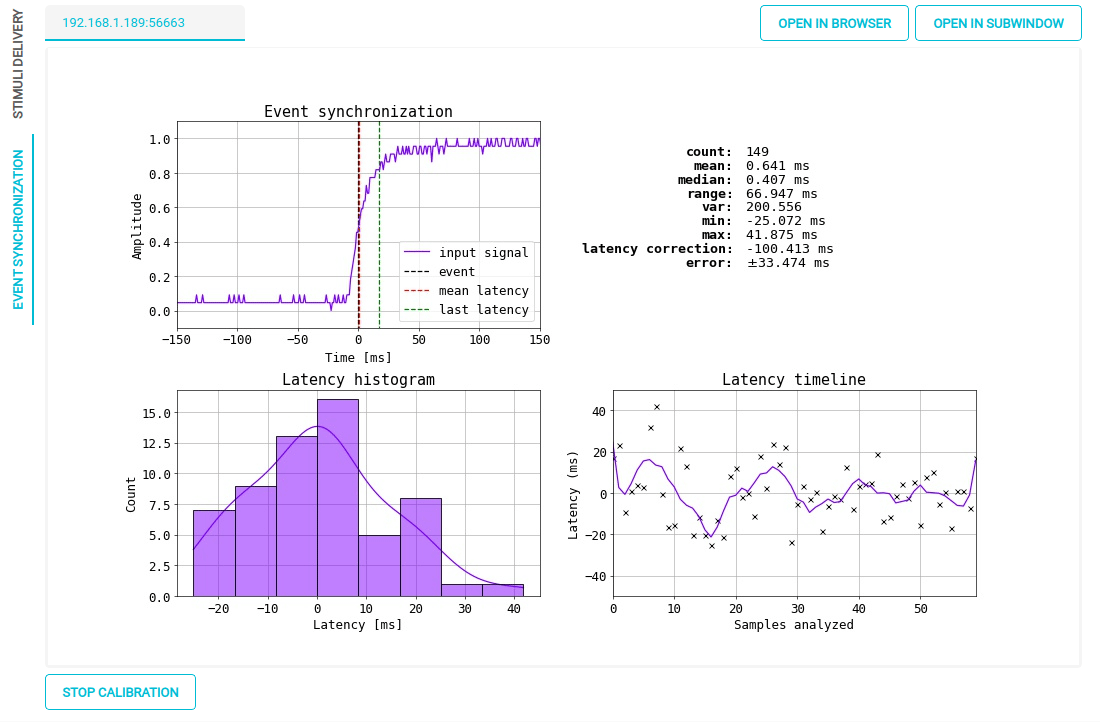
\includegraphics[width=0.8\textwidth]{Cap4/Figures/marker_sync.png}
\par\end{centering}
\caption[BCI-Framework: Marker synchronization]{BCI-Framework: Marker synchronization real-time interface.}
\label{fig:marker_sync}
\end{figure}

BCI-Framework integrates an interface to measure latencies and synchronize markers (Figure \ref{fig:marker_sync}), it was designed to be used on distributed environments. This simple latency correction consists of a stimuli delivery with only a marker synchronization area, the \gls*{LDR} module is constantly sensing (the boardmode must be in analog mode) so the changes on the square signal are compared with streamed markers and then the latency is corrected. The latency correction only affects the current instance, if BCI-Framework is restarted this calibration will be lose. For hard event synchronization, is prefer to use the markers synchronization constantly during all session.


%======================================================================
\section{Close the loop and Neurofeedback}

The BCI application with a close loop implementation consist of process in real-time the acquired data in order to execute commands in the real world. Although physiologically the close-loop signals differs from neurofeedback signals, since the nature of the data is different, the programmatically handle is exactly the same and are handled by \hyperref[ch4:feedbacks]{Feedbacks}. Once the feedback is defined through a method to perform asynchronous communication between them, the neurofeedback approaches can be implemented using this features. This implementation can be designed to run inside the interface, using \hyperref[ch4:rt_data_analysis]{Real-time data analysis} or to run isolated in no contextualized process. In Appendix \ref{appendix:neurofeedback} shows the implementation of a neurofeedback system.

The advantage to run process inside the framework is that this scrips share all the environment variables, and can be monitored through the main interface. On the other hand the scripts that run outside the framework only have access to the Kafka streams, this means that only can use the acquire data and are agnostics about everything else.




%======================================================================
\section{Summary and discussion}

BCI-Framework is the convergence of a set of drivers and tools working together to serve to the \textit{user} a full environment to acquire EEG signals and perform neurophysiological experiments with reliability and flexibility. Advance user can use the framework to develop custom visualizations and design paradigms that satisfy their needs using the integrated development environment. The main development was performed using Python, this feature brings to the framework one of the most complete computational libraries to work with data analysis and machine learning highly used to develop \gls*{BCI} systems today. 

The integrated development environment serve a full \gls*{API} with the main tasks automatized. The real-time data analysis and visualization build in background a fast system to buffering, sub-sampling and slice incoming EEG data en real-time. The stimuli delivery scripting has been designed to present views to the \textit{patient} asynchronously. In all cases the \textit{developer} only must care about the specific implementation of the analysis, visualizations and paradigm designed.

However the system only supports one acquisition board, \textit{OpenBCI Cyton}, although this is one of the most flexible and featured options available at the moment to write this thesis, the spreading of the framework tool could be seriously compromised. Also the main operating system focused, any based on \textit{GNU/Linux}, could be a reason that limits the adoption of the framework by the community.


    
    % IDK why but this line must be here
    \addtocontents{toc}{\protect\setcounter{tocdepth}{0}}
    
    \chapter{Final remarks}\label{ch:chapter_5}

%======================================================================
\section{Conclusions and discussion}

% outline
For this work were identified all components needed to get flexible, scalable, and integral  BCI system. Flexibility to adapt and modify experiments, make fast changes in runtime, and process data in real-time; Scalability in the execution of data analysis distributing expensive task without affect the main acquisition process; A framework that integrate a full environment with almost all tools to develop complete research-grade BCI systems.

% summary cap1
In order to guarantee all promised high features, a single board (\textit{OpenBCI Cyton}) was choose to be configured and controlled in deep. Then, a brand new set of drivers was developed with the capability to take advantage of the hardware and all benefits of the \textit{ADS1299}. The acquisition system support multiple sampling rate, packaging size, communication protocol, and free electrodes placement for use not only for \gls*{EEG} but \gls*{ECG} and \gls*{EMG}. Additional to this, a unique feature to synchronize markers had been included using the low levels characteristics of the acquisition board.

% summary cap2
Unlike the centralized systems that share the resources as well the stability. The distributed systems allow the controlled execution of a set of critical process like: The acquisition, the implementation of a dedicated system to handle the interaction with the OpenBCI hardware brings to the system robustness; the stimuli delivery, that allows pull apart the rendering and audiovisual generation to be able to stream markers and annotations in accurate times; and real-time data analysis, from experimental and not debugged scripts without the worry of causing exceptions in the system. Although it is a distributed system, the real-time streaming is guaranteed, the latency and the jitter keeps in accepted ranges for closed-loop \gls{BCI} systems, and acquisition methodology ensure that the bad sampling data can be labeled and processed as appropriate. 

% summary cap3
The development environment contribute with a full \gls*{API} and an automatic background to configure common task in the field of \gls{BCI} data processing like: buffering, sub-sampling and real-time trials slicing; an easy-to-use set of widgets to build dashboards for stimuli delivery; an environment to develop and debug custom extensions; and an interface to integrate the user develops alongside other extension at the same time. Implement neurofeedback paradigms and close-the-loop represent the most demanding and interesting tasks supported already in the system.


%======================================================================
\section{Future work} 

We have presented a framework to develop \gls*{BCI} systems with a lot of new features that are not present in state-of-art. However, there are still many issues that can be addressed to improve the performance, acceptance and the wide spreading of our system. In particular, the following aspects could be of interest for future work:

\begin{itemize}
    % Paralelo
    \item The electrodes density has always been one important discussion \cite{wang2016comparison, guo2020principles, liu2018detecting} in the field of \gls{BCI} systems. The proposed acquisition method has the potential to be parallelized and multiply the number of electrodes.
    
    % Acquisition system
    \item As well the selected board for this work, \textit{OpenBCI Cyton}, is one of the hardware with best performance and configurability, there is necessary a new acquisition board that integrates the most recent technology and communication protocols in a single board.
    
    % Multimodal
    \item The \gls*{SPRG} has recently interest in clinic multi-modal acquisition, BCI-Framework can be turn into a new framework to acquire and process real-time philological signals from multiple sources and serve visualizations, diagnostic support or store data.
    
    % Validación e implementacion en el grupo
    \item Although the system has been proven under specific applications and some databases has been generated (\href{appendix:motor-imagery}{Appendix: Motor imagery}, \href{appendix:working_memory}{Appendix: Visuospatial working memory - Change detection}) there is necessary more integration and validation with the methodologies developed the group. 
\end{itemize}



%======================================================================
\section{Academic products}

%----------------------------------------------------------------------
\subsection{Journal papers}
Paper submitted to \textit{SoftwareX - Journals | Elsevier} with the name "A real-time acquisition, visualization, and stimuli delivery Python-based tool for neurophysiological experiments"

%----------------------------------------------------------------------
\subsection{Patents}
The systems was submitted to the \textit{Crearlo no es suficiente} summons for a \textit{patentability search process} with the \textit{Universidad Nacional de Colombia sede Manizales} as main beneficiary, with the title "MÉTODO Y SISTEMA PARA LA SINCRONIZACIÓN DE MARCADORES ASOCIADOS A SISTEMAS DE INTERFAZ CEREBRO-COMPUTADOR", postulation ID \textit{343} and Application number \textit{NC2022/0007405} from May 28, 2022.

%----------------------------------------------------------------------
\subsection{Software registers}
A script developed with BCI-Framework for motor imagery paradigm based on games stimulus (Pacman interface), was submitted to software register in the textit{Universidad Nacional de Colombia sede Manizales}.

    
    % Appendix
    \renewcommand*{\TheAlphaChapter}{\Alph{chapter}}
    \begin{appendices}
        %======================================================================
\chapter{Python: Systemd service}\label{appendix:python_systemd_service}

\begin{description}
   \item[Description:]      Simple API to automate the creation of custom daemons for GNU/Linux.
   \item[License:]          BSD-2-clause
   \item[Latest version:]   \quot{1.8}
   \item[Python:]           \quot{3.8, 3.9, 3.10}
   \item[PyPi:]             \url{https://pypi.org/project/systemd-service/}
   \item[Repository:]       \url{https://github.com/UN-GCPDS/systemd-service}
   \item[Documentation:]    \url{https://systemd-service.readthedocs.io/en/latest/}
\end{description}
\hrulefill

A daemon is a service process that runs in the background and supervises the system or provides functionality to other processes. Traditionally, daemons are implemented following a scheme originating in SysV Unix \cite{daemon73:online}. Modern daemons should follow a simpler yet more powerful scheme, as implemented by systemd \cite{systemd78:online}.

\textit{Systemd service} is a Python module to automate the creation of Python-based daemons under GNU/Linux environments.


%======================================================================
\section{Install}
\begin{python}
pip install -U systemd-service
\end{python}


%======================================================================
\section{Handle daemons}
\begin{python}
from systemd_service import Service

daemon = Service("stream_rpyc")

daemon.stop()     # Start (activate) the unit.
daemon.start()    # Stop (deactivate) the unit.
daemon.reload()   # Reload the unit.  
daemon.restart()  # Start or restart the unit.

daemon.enable()   # Enable the unit.
daemon.disable()  # Disable the unit.

daemon.remove()   # Remove the file unit.
\end{python}
This commands are uquivalent to the \quot{systemctl} calls, for example run in terminal the folowing command:
\begin{python}
\$ systemctl enable stream_rpyc
\end{python}
Can be running inside a Python environment with using \quot{systemd\_service}
\begin{python}
from systemd_service import Service

daemon = Service("stream_rpyc")
daemon.enable()
\end{python}


%======================================================================
\section{Creating services}
Similar to the previous scripts, the services can be created using \quot{systemd\_service}:

\begin{python}
daemon = Service("stream_rpyc")
daemon.create_service()
\end{python}
If the service must be initialized after other service
\begin{python}
daemon = Service("stream_rpyc")
daemon.create_service(after='ntpd')
\end{python}


%======================================================================
\section{Creating timers}
Defines a timer relative to when the machine was booted up:
\begin{python}
daemon = Service("stream_rpyc")
daemon.create_timer(on_boot_sec=15)
\end{python}


%======================================================================
\section{Example}
This module is useful when is combined with package scripts declaration in \quot{setup.py} file:
\begin{python}
# setup.py

scripts=[
    "cmd/stream_rpyc",
]
\end{python}
The script could looks like:
\begin{python}
#!/usr/bin/env python

import sys

if sys.argv[-1] == "systemd":
    from systemd_service import Service
    daemon = Service("stream_rpyc")
    daemon.create_timer(on_boot_sec=10, after='network.target kafka.service')

else:
    from my_module.submodule import my_service
    print("Run 'stream_rpyc systemd' as superuser to create the daemon.")
    my_service()
\end{python}
Then the command can be called as a simple script but with the \quot{systemd} argument the command will turn into a service.
\begin{python}
\$ stream_rpyc
# Command executed normally
\end{python}
\begin{python}
\$ stream_rpyc systemd
# Service created
\end{python}
        %======================================================================
\chapter{Python: Qt-Material}\label{appendix:qt-material}

\begin{description}
   \item[Description:]      Material inspired stylesheet for PySide2, PySide6, PyQt5 and PyQt6.
   \item[License:]          BSD-2-clause
   \item[Latest version:]   \quot{2.12}
   \item[Python:]           \quot{3.8, 3.9, 3.10}
   \item[PyPi:]             \url{https://pypi.org/project/qt-material/}
   \item[Repository:]       \url{https://github.com/UN-GCPDS/qt-material}
   \item[Documentation:]    \url{https://qt-material.readthedocs.io/en/latest/}
\end{description}
\hrulefill

This is another stylesheet for PySide6, PySide2, PyQt5 and PyQt6, which looks like Material Design (close enough).

\begin{figure}
\begin{centering}
% \includesvg[width=0.8\textwidth]{Cap4/Figures/transformer.svg}
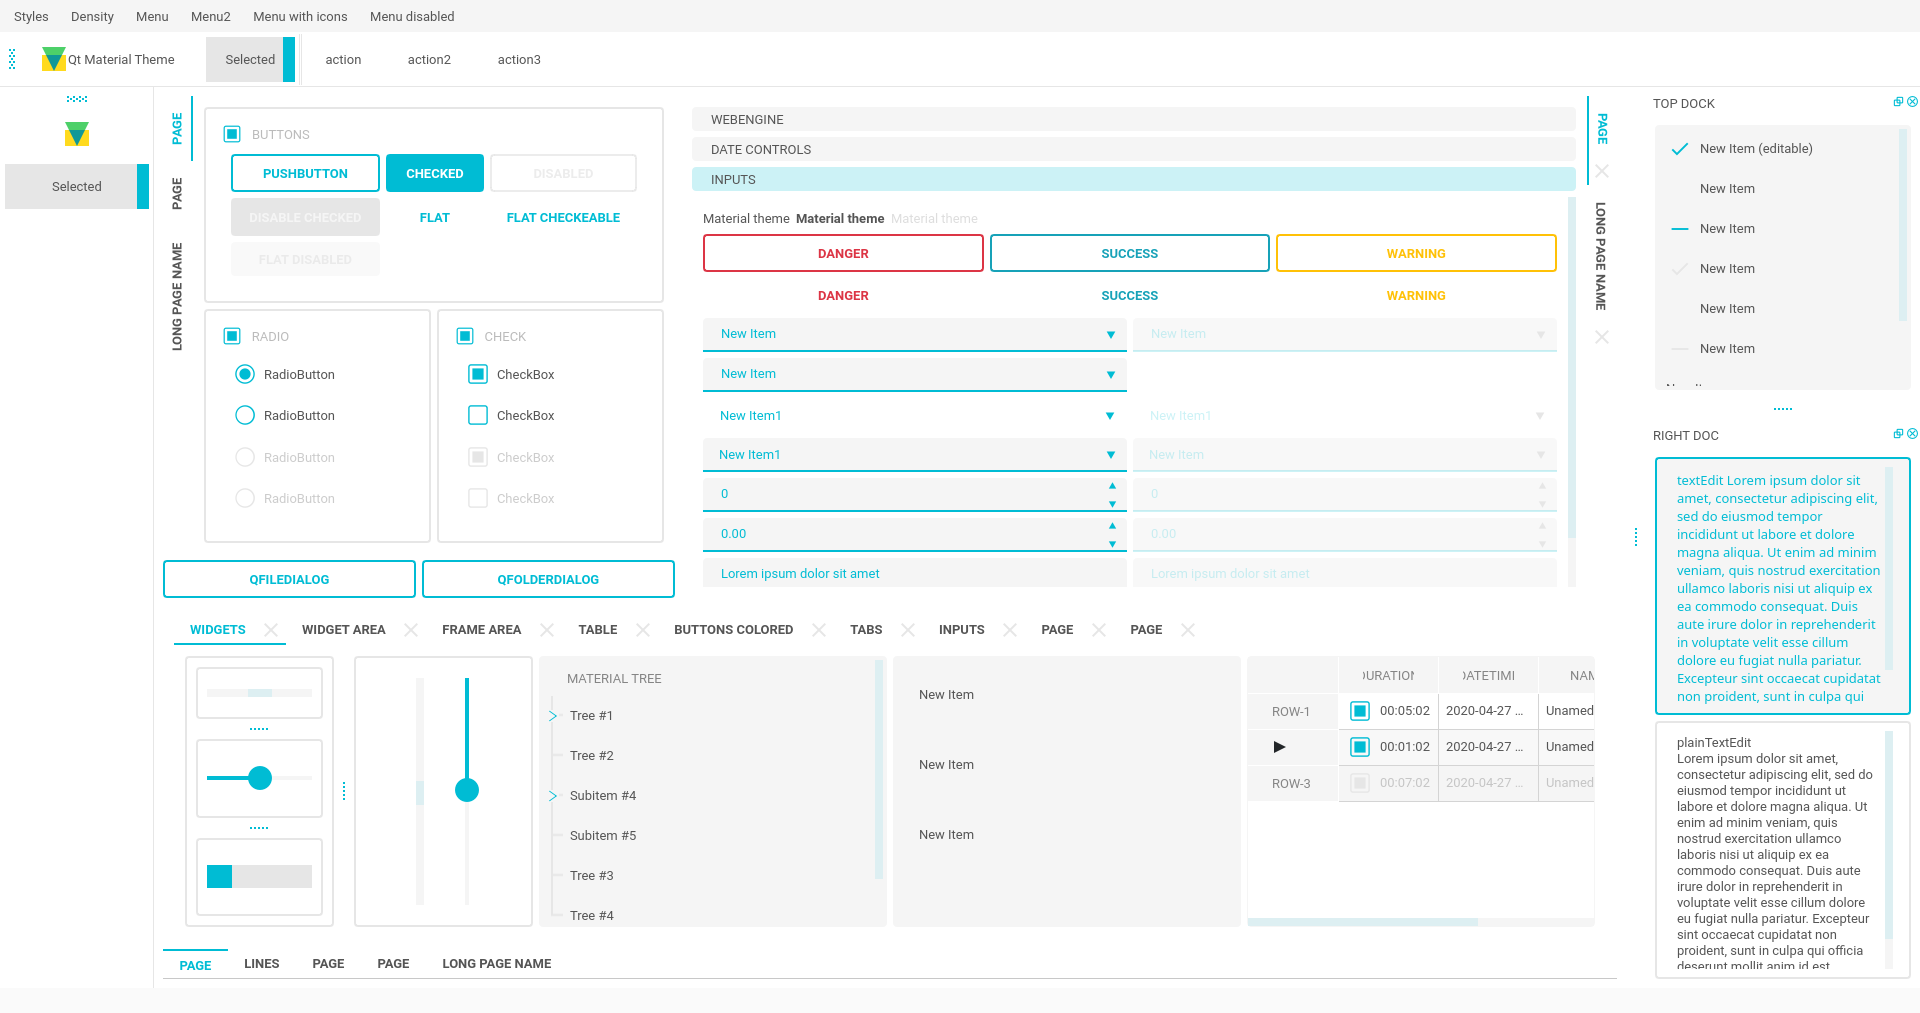
\includegraphics[width=1\textwidth]{Appendix/python_modules/Figures/qt-light_cyan_500.png}
\par\end{centering}
\caption[\textit{light\_cyan\_500.xml} theme for Qt-Material]{\textit{light\_cyan\_500.xml} theme for Qt-Material.}
\label{fig:qt-light_cyan_500}
\end{figure}

%======================================================================
\section{Install}
\begin{python}
pip install -U qt-material
\end{python}

%======================================================================
\section{Usage}
\begin{python}
import sys
from PySide6 import QtWidgets
# from PySide2 import QtWidgets
# from PyQt5 import QtWidgets
from qt_material import apply_stylesheet

# create the application and the main window
app = QtWidgets.QApplication(sys.argv)
window = QtWidgets.QMainWindow()

# setup stylesheet
apply_stylesheet(app, theme='dark_teal.xml')

# run
window.show()
app.exec_()
\end{python}
\
%======================================================================
\section{Themes}
\begin{python}
from qt_material import list_themes

list_themes()
\end{python}
\begin{python}
['dark_amber.xml',
 'dark_blue.xml',
 'dark_cyan.xml',
 'dark_lightgreen.xml',
 'dark_pink.xml',
 'dark_purple.xml',
 'dark_red.xml',
 'dark_teal.xml',
 'dark_yellow.xml',
 'light_amber.xml',
 'light_blue.xml',
 'light_cyan.xml',
 'light_cyan_500.xml',
 'light_lightgreen.xml',
 'light_pink.xml',
 'light_purple.xml',
 'light_red.xml',
 'light_teal.xml',
 'light_yellow.xml']
\end{python}

%======================================================================
\section{Custom colors}
\footcite{Color Tool}{https://material.io/resources/color/#!/?view.left=0&view.right=0} is the best way to generate new themes, just choose colors and export as \quot{Android XML}, the theme file must look like:
\begin{python}
<!--?xml version="1.0" encoding="UTF-8"?-->
<resources>
<color name="primaryColor">#00e5ff</color>
<color name="primaryLightColor">#6effff</color>
<color name="secondaryColor">#f5f5f5</color>
<color name="secondaryLightColor">#ffffff</color>
<color name="secondaryDarkColor">#e6e6e6</color>
<color name="primaryTextColor">#000000</color>
<color name="secondaryTextColor">#000000</color>
</resources>
\end{python}

Save it as \quot{my\_theme.xml} or similar and apply the style sheet from Python.

\begin{python}
apply_stylesheet(app, theme='dark_teal.xml')
\end{python}


%======================================================================
\section{Light themes}
Light themes will need to add \quot{invert\_secondary} argument as \quot{True}.
\begin{python}
apply_stylesheet(app, theme='light_red.xml', invert_secondary=True)
\end{python}


%======================================================================
\section{Environ variables}
There is a environ variables related to the current theme used, these variables are for consult purpose only.

% Preview source code for paragraph 18

\begin{table}[H]
\begin{centering}
\begin{tabular}{>{\raggedright}m{5cm}>{\raggedright}m{5cm}>{\raggedright}m{2cm}}
\toprule 
\addlinespace[1em]
\textbf{Environ variable} & \textbf{Description} & \textbf{Example}\tabularnewline\addlinespace[1em]
\midrule
\quottable{QTMATERIAL\_PRIMARYCOLOR}  & Primary color  & \quottable{\#2979ff}\tabularnewline
\addlinespace[0.5cm]
\quottable{QTMATERIAL\_PRIMARYLIGHTCOLOR} & A bright version of the primary color & \quottable{\#75a7ff}\tabularnewline
\addlinespace[0.5cm]
\quottable{QTMATERIAL\_SECONDARYCOLOR} & Secondary color & \quottable{\#f5f5f5}\tabularnewline
\addlinespace[0.5cm]
\quottable{QTMATERIAL\_SECONDARYLIGHTCOLOR}  & A bright version of the secondary color  & \quottable{\#ffffff} \tabularnewline
\addlinespace[0.5cm]
\quottable{QTMATERIAL\_SECONDARYDARKCOLOR}  & A dark version of the primary color  & \quottable{\#e6e6e6} \tabularnewline
\addlinespace[0.5cm]
\quottable{QTMATERIAL\_PRIMARYTEXTCOLOR}  & Color for text over primary background  & \quottable{\#000000} \tabularnewline
\addlinespace[0.5cm]
\quottable{QTMATERIAL\_SECONDARYTEXTCOLOR} & Color for text over secondary background  & \quottable{\#000000} \tabularnewline
\addlinespace[0.5cm]
\quottable{QTMATERIAL\_THEME} & Name of theme used  & \quottable{"light\_blue.xml"}\tabularnewline
\bottomrule
\addlinespace[0.5cm]
\end{tabular}
\par\end{centering}
\caption{Environ variables defined by Qt-Material.\label{table:environ_vars}}
\end{table}



%======================================================================
\section{Alternative QPushButtons and custom fonts}
There is an \quot{extra} argument for accent colors and custom fonts.
\begin{python}
extra = {

    # Button colors
    'danger': '#dc3545',
    'warning': '#ffc107',
    'success': '#17a2b8',

    # Font
    'font_family': 'Roboto',
}

apply_stylesheet(app, 'light_cyan.xml', invert_secondary=True, extra=extra)
\end{python}
The accent colors are applied to \quot{QPushButton} with the corresponding \quot{class} property:
\begin{python}
pushButton_danger.setProperty('class', 'danger')
pushButton_warning.setProperty('class', 'warning')
pushButton_success.setProperty('class', 'success')
\end{python}

\begin{figure}[H]
\begin{centering}
% \includesvg[width=0.8\textwidth]{Cap4/Figures/transformer.svg}
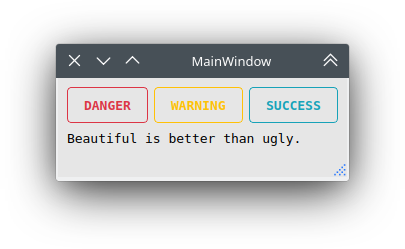
\includegraphics[width=0.6\textwidth]{Appendix/python_modules/Figures/qt-extra.png}
\par\end{centering}
\caption{QPushButtons stylized with class property.}
\label{fig:qt-extra}
\end{figure}

%======================================================================
\section{Custom stylesheets}
Custom changes can be performed by overwriting the stylesheets, for example:
\begin{python}
QPushButton {{
  color: {QTMATERIAL_SECONDARYCOLOR};
  text-transform: none;
  background-color: {QTMATERIAL_PRIMARYCOLOR};
}}

.big_button {{
  height: 64px;
}}
\end{python}
Then, the current stylesheet can be extended just with:
\begin{python}
apply_stylesheet(app, theme='light_blue.xml')

stylesheet = app.styleSheet()
with open('custom.css') as file:
    app.setStyleSheet(stylesheet + file.read().format(**os.environ))
\end{python}
And the class style can be applied with the \quot{setProperty} method:
\begin{python}
self.main.pushButton.setProperty('class', 'big_button')
\end{python}

\begin{figure}[H]
\begin{centering}
% \includesvg[width=0.8\textwidth]{Cap4/Figures/transformer.svg}
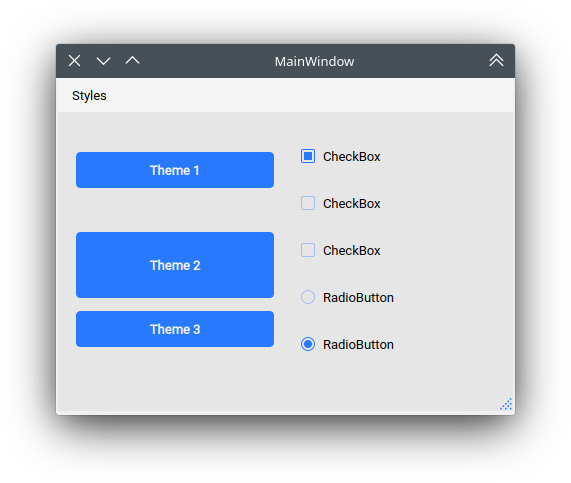
\includegraphics[width=0.7\textwidth]{Appendix/python_modules/Figures/qt-custom.png}
\par\end{centering}
\caption{QPushButtons stylized with user defined class property.}
\label{fig:qt-custom}
\end{figure}

%======================================================================
\section{Run examples}\
A window with almost all widgets (see the previous screenshots) are available to test all themes and create new ones.
\begin{python}
git clone https://github.com/UN-GCPDS/qt-material.git
cd qt-material
python setup.py install
cd examples/full_features
python main.py --pyside6
\end{python}

%======================================================================
\section{Change theme in runtime}
There is a \quot{qt\_material.QtStyleTools} class that must be inherited along to QMainWindow for change themes in runtime using the \quot{apply\_stylesheet()} method.
\begin{python}
class RuntimeStylesheets(QMainWindow, QtStyleTools):
    
    def __init__(self):
        super().__init__()
        self.main = QUiLoader().load('main_window.ui', self)
        
        self.apply_stylesheet(self.main, 'dark_teal.xml')
        # self.apply_stylesheet(self.main, 'light_red.xml')
        # self.apply_stylesheet(self.main, 'light_blue.xml')
\end{python}

%======================================================================
\section{Integrate stylesheets in a menu}
A custom stylesheets menu can be added to a project for switching across all default available themes.
\begin{python}
class RuntimeStylesheets(QMainWindow, QtStyleTools):
    
    def __init__(self):
        super().__init__()
        self.main = QUiLoader().load('main_window.ui', self)
        
        self.add_menu_theme(self.main, self.main.menuStyles)
\end{python}


%======================================================================
\section{Create new themes}
A simple interface is available to modify a theme in runtime, this feature can be used to create a new theme, the theme file is created in the main directory as \quot{my\theme.xml}
\begin{python}
class RuntimeStylesheets(QMainWindow, QtStyleTools):
    
    def __init__(self):
        super().__init__()
        self.main = QUiLoader().load('main_window.ui', self)
        
        self.show_dock_theme(self.main)
\end{python}
A full set of examples are available in the \citefoot{exmaples directory}{https://github.com/UN-GCPDS/qt-material/blob/master/examples/runtime/}

%======================================================================
\section{Export theme}
This feature able to use \textit{Qt-Material} themes into \quot{Qt} implementations using only local files.
\begin{python}
from qt_material import export_theme

extra = {

    # Button colors
    'danger': '#dc3545',
    'warning': '#ffc107',
    'success': '#17a2b8',

    # Font
    'font_family': 'monoespace',
    'font_size': '13px',
    'line_height': '13px',

    # Density Scale
    'density_scale': '0',

    # environ
    'pyside6': True,
    'linux': True,

}

export_theme(theme='dark_teal.xml', 
             qss='dark_teal.qss', 
             rcc='resources.rcc',
             output='theme', 
             prefix='icon:/', 
             invert_secondary=False, 
             extra=extra,
            )
\end{python}
This script will generate both \quot{dark\_teal.qss} and \quot{resources.rcc} and a folder with all theme icons called \quot{theme}.

The files generated can be integrated into a \quot{PySide6} application just with:
\begin{python}
import sys

from PySide6 import QtWidgets
from PySide6.QtCore import QDir
from __feature__ import snake_case, true_property

# Create application
app = QtWidgets.QApplication(sys.argv)

# Load styles
with open('dark_teal.qss', 'r') as file:
    app.style_sheet = file.read()

# Load icons
QDir.add_search_path('icon', 'theme')

# App
window = QtWidgets.QMainWindow()
checkbox = QtWidgets.QCheckBox(window)
checkbox.text = 'CheckBox'
window.show()
app.exec()
\end{python}
This files can also be used into non \quot{Python} environs like \quot{C++}.

%======================================================================
\section{Density scale}
The \quot{extra arguments} also include an option to set the \textit{density scale}, by default is \quot{0}.
\begin{python}
extra = {
    
    # Density Scale
    'density_scale': '-2',
}

apply_stylesheet(app, 'default', invert_secondary=False, extra=extra)
\end{python}

        %======================================================================
\chapter{Python: Matplotlib-FigureStream}\label{appendix:matplotlib-figurestream}

\begin{description}
   \item[Description:]      A backend for serve Matplotlib animations as web streams.
   \item[License:]          BSD-2-clause
   \item[Latest version:]   \quot{1.2.6}
   \item[Python:]           \quot{3.8, 3.9, 3.10}
   \item[PyPi:]             \url{https://pypi.org/project/figurestream/}
   \item[Repository:]       \url{https://github.com/UN-GCPDS/matplotlib-figurestream}
   \item[Documentation:]    \url{https://figurestream.readthedocs.io/en/latest/}
\end{description}
\hrulefill

%======================================================================
\section{Install}
\begin{python}
pip install -U figurestream
\end{python}

%======================================================================
\section{Bare minimum}
By default, the stream serves on \url{http://localhost:5000}

\begin{python}
# FigureStream replace any Figure object
from figurestream import FigureStream

import numpy as np
from datetime import datetime

# FigureStream can be used like any Figure object
stream = FigureStream()
sub = stream.add_subplot(111)
x = np.linspace(0, 3, 1000)

# Update animation loop
while True:
    sub.clear()  # clear the canvas

    # ------------------------------------------------------------------------
    # Any plot operation
    sub.set_title('FigureStream')
    sub.set_xlabel('Time [s]')
    sub.set_ylabel('Amplitude')
    sub.plot(x, np.sin(2 * np.pi * 2 * (x + datetime.now().timestamp())))
    sub.plot(x, np.sin(2 * np.pi * 0.5 * (x + datetime.now().timestamp())))
    # ------------------------------------------------------------------------

    stream.feed()  # push the frame into the server
\end{python}

For fast updates is recommended to use \quot{set\_data}, \quot{set\_ydata} and \quot{set\_xdata} instead of clear and draw again in each loop, also \quot{FigureStream} can be implemented from a custom class.

\begin{python}
# FigureStream replace any Figure object
from figurestream import FigureStream

import numpy as np
from datetime import datetime


class FastAnimation(FigureStream):
    def __init__(self, *args, **kwargs):
        super().__init__(*args, **kwargs)

        axis = self.add_subplot(111)
        self.x = np.linspace(0, 3, 1000)

        # ---------------------------------------------------------------------
        # Single time plot configuration
        axis.set_title('FigureStream')
        axis.set_xlabel('Time [s]')
        axis.set_ylabel('Amplitude')

        axis.set_ylim(-1.2, 1.2)
        axis.set_xlim(0, 3)

        # Lines objects
        self.line1, *_ = axis.plot(self.x, np.zeros(self.x.size))
        self.line2, *_ = axis.plot(self.x, np.zeros(self.x.size))
        # ---------------------------------------------------------------------

        self.anim()

    def anim(self):
        # Update animation loop
        while True:
            # -----------------------------------------------------------------
            # Update only the data values is faster than update all the plot
            self.line1.set_ydata(
                np.sin(2 * np.pi * 2 * (self.x + datetime.now().timestamp()))
            )
            self.line2.set_ydata(
                np.sin(
                    2 * np.pi * 0.5 * (self.x + datetime.now().timestamp())
                )
            )
            # -----------------------------------------------------------------

            self.feed()  # push the frame into the server


if __name__ == '__main__':
    FastAnimation()

\end{python}

%======================================================================
\section{Set host, port and endpoint}
If we want to serve the stream in a different place we can use the parameters \quot{host}, \quot{port} and \quot{endpoint}, for example:
\begin{python}
FigureStream(host='0.0.0.0', port='5500', endpoint='figure.jpeg')
\end{python}

Now the stream will serve on \url{http://localhost:5500/figure.jpeg} and due the \quot{0.0.0.0} host is accesible for any device on network.
By default \quot{host} is \quot{localhost}, \quot{port} is \quot{5000} and \quot{endpoint} is empty.

        %======================================================================
\chapter{Python/Brython: Radiant framework}\label{appendix:brython-radiant}

\begin{description}
   \item[Description:]      A Brython Framework for Web Apps development.
   \item[License:]          BSD-2-clause
   \item[Latest version:]   \quot{3.3.8}
   \item[Python:]           \quot{3.8, 3.9, 3.10}
   \item[PyPi:]             \url{https://pypi.org/project/radiant/}
   \item[Repository:]       \url{https://github.com/UN-GCPDS/brython-radiant}
   \item[Documentation:]    \url{https://radiant-framework.readthedocs.io/en/latest/}
\end{description}
\hrulefill

Radiant is a \footcite{Brython}{https://brython.info/} framework for the quick development of web apps with pure Python/Brython syntax so there is no need to care about (if you don’t want) HTML, CSS, or Javascript. Run over \footcite{Tornado}{https://www.tornadoweb.org/} servers and include support to \textit{Websockets}, \textit{Python Scripts} and \textit{MDC}.


%======================================================================
\section{Install}
\begin{python}
pip install -U radiant
\end{python}


%======================================================================
\section{Bare minimum}
\begin{python}
# Radiant modules
from radiant.server import RadiantAPI

# Brython modules
# This modules are faked after `radiant` import
from browser import document, html  

# Main class inheriting RadiantAPI
class BareMinimum(RadiantAPI):

    # Constructor
    def __init__(self, *args, **kwargs):
        super().__init__(*args, **kwargs)

        #-----------------------------------------------------------
        # Brython code (finally)
        document.select_one('body') <= html.H1('Hello World')
        #
        # ...all your brython code
        #-----------------------------------------------------------

# Run server
if __name__ == '__main__':
    BareMinimum()
\end{python}


%======================================================================
\section{Extra options}
\begin{python}
# Radiant modules
# Import RadiantServer for advanced options
from radiant.server import RadiantAPI, RadiantServer  

from browser import document, html

# Main class inheriting RadiantAPI
class BareMinimum(RadiantAPI):

    def __init__(self, *args, **kwargs):
        """"""
        super().__init__(*args, **kwargs)

        #-----------------------------------------------------------
        # Brython code
        document.select_one('body') <= html.H1('Hello World')
        #
        # ...all your brython code
        #-----------------------------------------------------------

if __name__ == '__main__':
    # Advance options
    RadiantServer('BareMinimum',
                  host='localhost',
                  port=5000,
                  brython_version='3.9.1',
                  debug_level=0,
                  )
\end{python}


%======================================================================
\section{How to works}
This is basically a set of scripts that allows the same file run from \textit{Python} and \textit{Brython}, when is running under \textit{Python} a \textit{Tornado} server is created and configure the local path for serving static files, and a custom \textit{HTML} template is configured in runtime to import the same script, this time under \textit{Brython}, is very simple.


%======================================================================
\section{WebSockets}
This WebSockets are in the Tornado side and NOT in Brython. So, is basically and \footcite{WebSocketHandler}{https://www.tornadoweb.org/en/stable/websocket.html} object like:

\begin{python}
#ws_handler.py

from tornado.websocket import WebSocketHandler

class WSHandler(WebSocketHandler):

    def open(self):
        ...

    def on_close(self):
        ...

    def on_message(self, message):
        ...
\end{python}

That can be included with the \quot{RadiantServer} class in the \quot{websockethandler} argument:
\begin{python}
RadiantServer('MainApp', websockethandler=('ws_handler.py', 'WSHandler'))
\end{python}

This websocket will be serving on \quot{/ws} URL.

%======================================================================
\section{Python scripting}
This feature is to run a real Python environment through methods that return objects. make sure to inherit \quot{PythonHandler}:
\begin{python}
#python_foo.py

from radiant import PythonHandler

class MyClass(PythonHandler):

    def local_python(self):
        return "This file are running from Local Python environment"

    def pitagoras(self, a, b):
        return math.sqrt(a ** 2 + b ** 2)
\end{python}
This handler can be included with the \quot{RadiantServer} class in the \quot{python} argument:
\begin{python}
RadiantServer('MainApp', python=('python_foo.py', 'MyClass'))
\end{python}
A full example of use could be:
\begin{python}
from radiant import RadiantAPI, RadiantServer
from browser import document, html

class MainApp(RadiantAPI):

    def __init__(self, *args, **kwargs):
        super().__init__(*args, **kwargs)

        document.select('body')[0] <= html.H1('Hello World')
        document.select('body')[0] <= html.H3(self.MyClass.local_python())

        a, b = 3, 5
        c = self.MyClass.pitagoras(a, b)
        document.select('body')[0] <= html.H3(f"Pitagoras: {a=}, {b=}, {c=:.3f}")

if __name__ == '__main__':
    RadiantServer('MainApp', python=('python_foo.py', 'MyClass'))
\end{python}


%======================================================================
\section{Custom themes}
Material themes from MDC can be configured with \footcite{Color Tool}{https://material.io/resources/color/} application, just select the desired colors, save the file and add it to the \quot{RadiantServer} class in the attribute \quot{theme}.
\begin{python}
RadiantServer('MainApp', theme='custom_theme.xml')
\end{python}

        %======================================================================
\chapter{Database: Motor imagery}\label{appendix:motor-imagery}

\begin{description}
   \item[Description:]      Motor Imagery database.
   \item[Subjects:]         \quot{7}
   \item[License:]          CC BY-NC-ND 4.0
   \item[Repository:]       \url{https://github.com/UN-GCPDS/}
\end{description}
\hrulefill

\gls*{MI} is the process of imagining a motor action without any motor execution. During an \gls*{MI} task, a subject visualizes in their mind an instructed motor action, i.e., to move the right hand, without actually carrying it out. When subjects plan and execute movements, characteristic rhythms in the sensorimotor areas, typically the $\mu$ or precentral $\alpha$ rhythm (8–12 Hz) and the $\beta$ rhythm (13–30 Hz), get activated \cite{xu2020two}. That is to say, \gls*{MI} and motor execution share common sensorimotor areas, and both involve envisioning and executing the same motor plan \cite{garcia2021single}. Although, their neural mechanisms seem to have some differences \cite{matsuo2021comparison}. Assessing and interpreting \gls*{MI} brain dynamics may contribute to applications like the evaluation of pathological conditions, the rehabilitation of motor functions, and motor learning and performance \cite{collazos2020cnn}. Particularly, much attention has been paid in the literature to \gls*{BCI} systems that can decode \gls*{MI}-associated task patterns, usually captured through scalp EEG signals, and translate them into commands in order to control external devices \cite{galindo2020multiple, xu2020two}. One the main limitations for the widespread use of such systems being that about 15–30\% of users display \gls*{BCI} illiteracy, i.e. they do not gain enough control over the interfaces, possibly because subjects with poor control performance do not exhibit discriminative task-related changes over the modulation of sensorimotor rhythms during the interval of \gls*{MI} responses \cite{garcia2021single}.

%======================================================================
\section{Paradigm}
This cue-based \gls*{BCI} paradigm consisted of up to four different motor imagery tasks, represented by a succession of cues (arrow-shaped) and separated with an asynchronous break. This paradigm used an arrow pointing to the left right, up or bottom, which has been widely used \cite{choi2013electroencephalography, llanos2013mu}.

\begin{figure}[H]
\begin{centering}
% \includesvg[width=0.8\textwidth]{Cap4/Figures/transformer.svg}
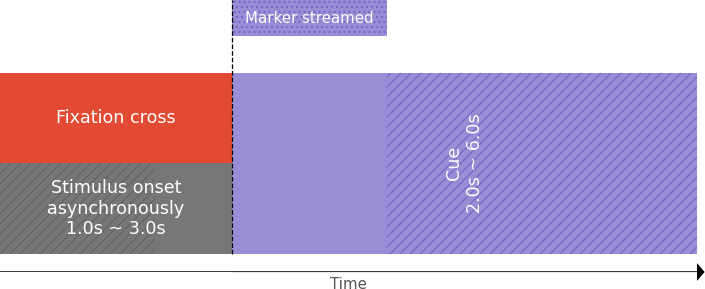
\includegraphics[width=1\textwidth]{Appendix/databases/Figures/mi-paradigm.png}
\par\end{centering}
\caption{\gls*{MI} paradigm implementation with markers indicators.}
\label{}
\end{figure}

%======================================================================
\section{Stimuli presentation}
There is two kind of cues for the \gls{MI} stimuli delivery, the first one is based on the classic arrows and the second one use Pacman-based cues. Both of the paradigms were build with a dashboard that can be used to configure the experiment times.
\begin{figure}[H]
\begin{centering}
% \includesvg[width=0.8\textwidth]{Cap4/Figures/transformer.svg}
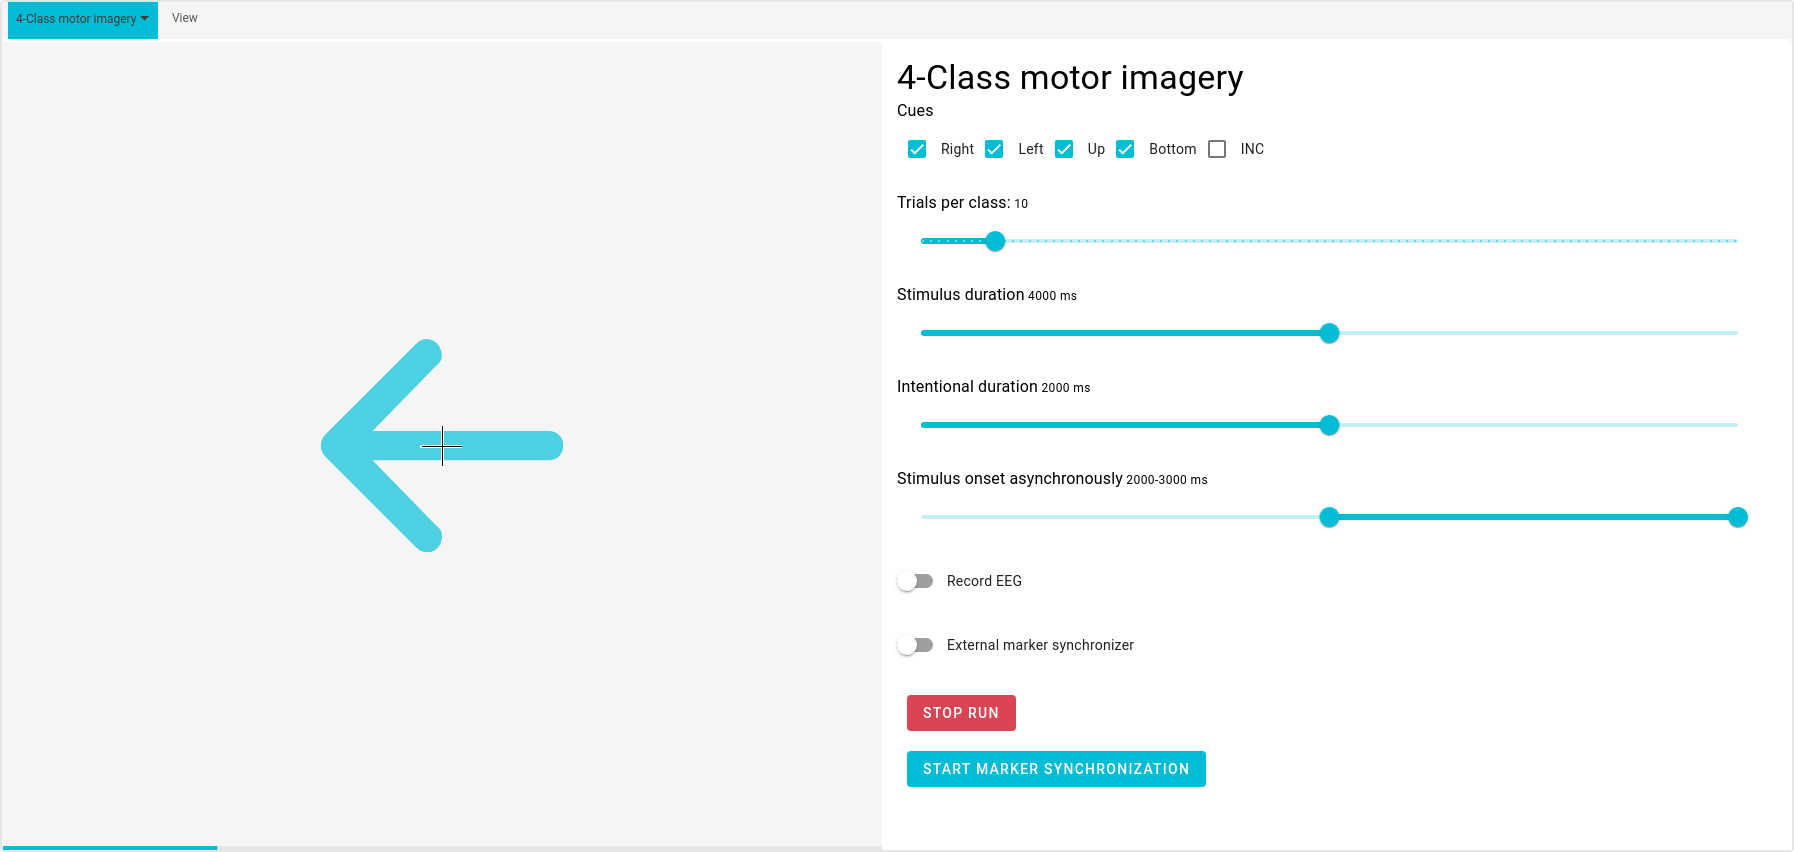
\includegraphics[width=1\textwidth]{Appendix/databases/Figures/mi-delivery.png}
\par\end{centering}
\caption{\gls*{MI} stimuli delivery interface with arrow cues.}
\label{}
\end{figure}

The Pacman-based cues use a clean interface in order to prevent unintentional stimulation, then all screen indicators like time, score, level and bonus were removed. 
\begin{figure}[H]
\begin{centering}
% \includesvg[width=0.8\textwidth]{Cap4/Figures/transformer.svg}
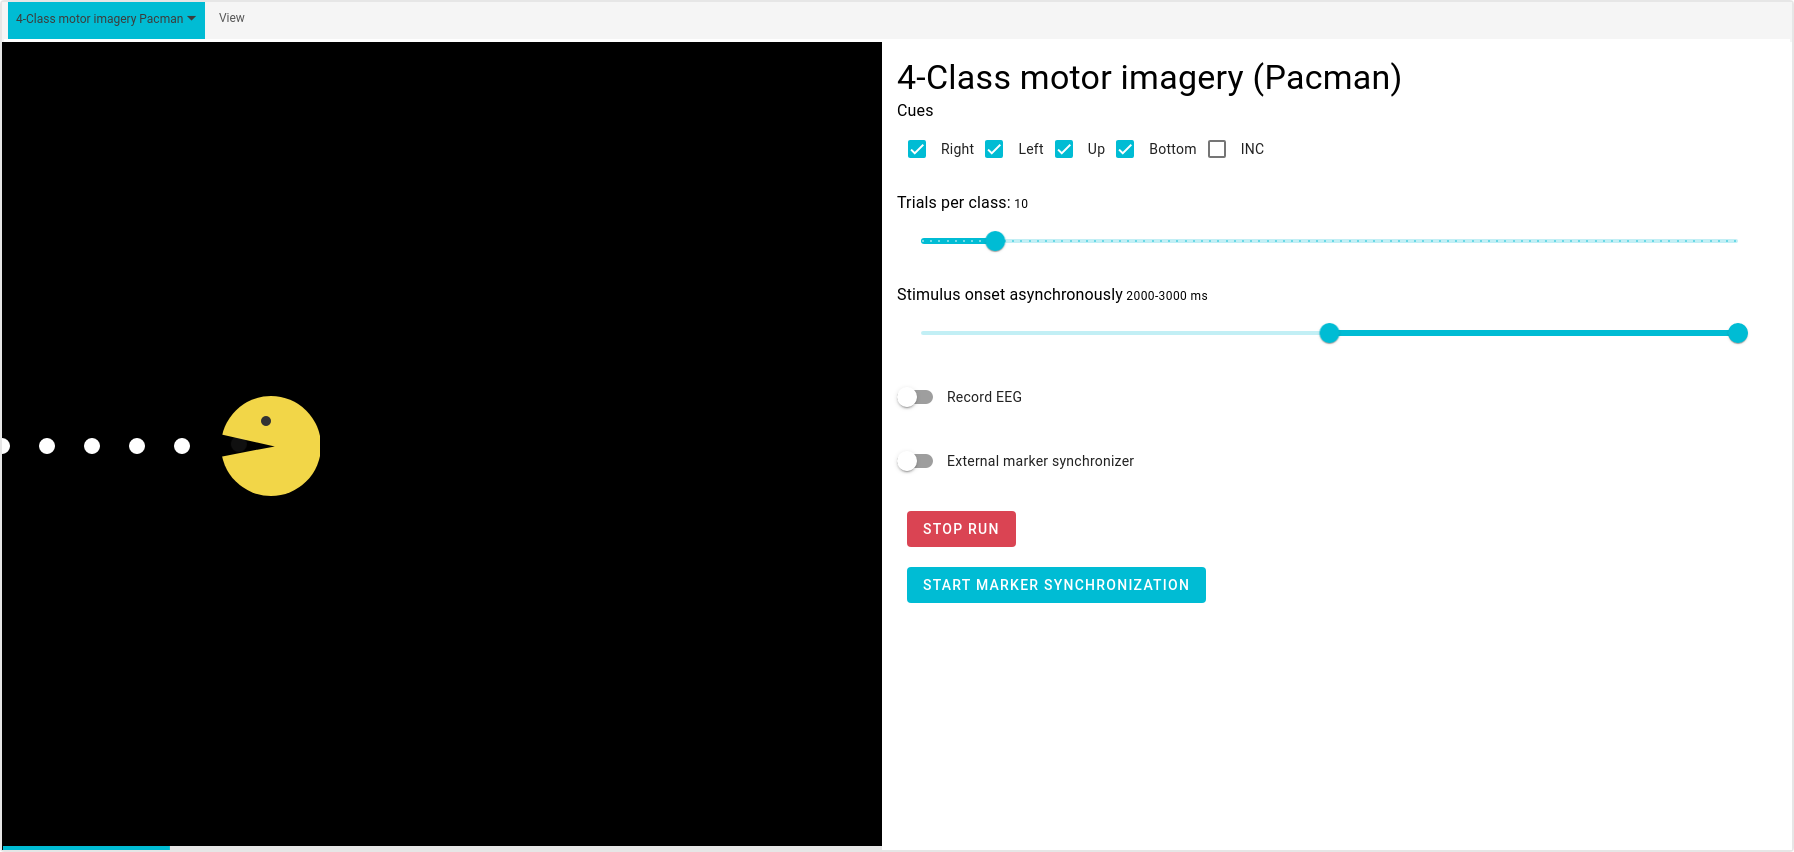
\includegraphics[width=1\textwidth]{Appendix/databases/Figures/mi-delivery-pacman.png}
\par\end{centering}
\caption{\gls*{MI} stimuli delivery interface with pacman-base cues.}
\label{}
\end{figure}


%======================================================================
\section{Intention detection}
An additional feature were included into this paradigm, an intentional detection, the cue add an stimuli indicating the next task, the subject must be instructed about not perform any activity. The intentional detection, this task also has interest in the field of the motor execution.

\begin{figure}[H]
\begin{centering}
% \includesvg[width=0.8\textwidth]{Cap4/Figures/transformer.svg}

\includegraphics[width=1\textwidth]{Appendix/databases/Figures/mi-intentional.png}
\par\end{centering}
\caption{\gls*{MI} with intentional detection.}
\label{}
\end{figure}

%======================================================================
\section{Motor imagery with intentional non-control stimulus}
Other experimental feature included in the stimuli delivery was the intentional non-control \cite{perdikis2014subject}, this feature is useful to close the loop, since in real implementations there are situations were the patient do not want to perform any action. This new cue is modeled as a circle. 

\begin{figure}[H]
\begin{centering}
% \includesvg[width=0.8\textwidth]{Cap4/Figures/transformer.svg}

\includegraphics[width=1\textwidth]{Appendix/databases/Figures/mi-nonintentional.png}
\par\end{centering}
\caption{\gls*{MI} with nonintentional stimulus.}
\label{}
\end{figure}

        %======================================================================
\chapter{Database: Visuospatial working memory - Change detection task}\label{appendix:working_memory}

\begin{description}
   \item[Description:]      Visuospatial working memory database.
   \item[Subjects:]         \quot{4}
   \item[License:]          CC BY-NC-ND 4.0
   \item[Repository:]       \url{https://github.com/UN-GCPDS/}
\end{description}
\hrulefill

\gls*{VWM} is a memory system of limited capacity with the ability to store and manipulate information for a short period of time \cite{baddeley2017working, pavlov2022oscillatory}. It plays a key role in complex cognitive tasks such as comprehension, reasoning, planning and learning \cite{johnson2019spectral, zhang2016functional}, as well as in daily activities such as problem solving and decision-making \cite{dai2017eeg}. \gls{VWM} consists of three distinct stages of information processing: encoding, maintenance or retention, and retrieval \cite{johnson2018dynamic}, with the retention interval being considered as a defining component of \gls{VWM}, since it differentiates it from other memory types \cite{pavlov2022oscillatory}. 

%======================================================================
\section{Paradigm}
The task consists in remembering the colors of a set of squares displayed on a computer screen, termed memory array, and then comparing them with the colors of a second set of squares located in the same positions, termed test array \cite{vogel2004neural}. A trial of the task begins with an arrow indicating either the left or the right side of the screen for 0.2 s. Then, a memory array appears on the screen for 0.1 s. For every trial, memory arrays are displayed on both hemifields, but the subject must remember only those appearing on the side indicated by the arrow cue. Next, after a retention interval lasting 0.9 s, a test array appears for a period of 2 s. During this period the subject reports if the colors of all the items in the memory and test arrays match. The task has three levels according to the number of elements in the memory array: low memory load (one square), medium memory load (two squares), and high memory load (four squares). The subject must perform a total of 300 trials, with 100 trials for each memory load level (50 trials per hemifield). Trials from different levels are presented at random. The color of one of the squares in the test array differs from its counterpart in the memory array in 50\% of the trials.

\begin{figure}[H]
\begin{centering}
% \includesvg[width=0.8\textwidth]{Cap4/Figures/transformer.svg}
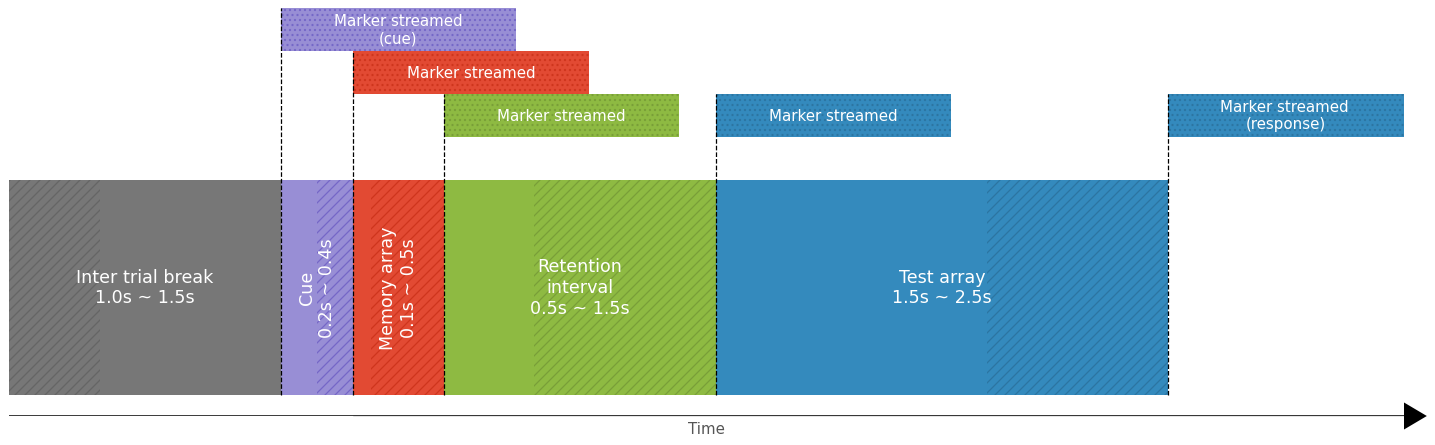
\includegraphics[width=1\textwidth]{Appendix/databases/Figures/vwm-paradigm.png}
\par\end{centering}
\caption{\gls*{VWM} paradigm implementation with markers indicators.}
\label{}
\end{figure}


%======================================================================
\section{Stimuli presentation}
All stimuli are presented on a computer screen situated 120 cm away from the subject. The stimulus arrays appear within two $7.2^{\circ}$ × $13.15^{\circ}$ rectangular regions that are centered $5.4^{\circ}$ to the left and right of a central fixation cross on a gray background (the symbol $\circ$ stands for degrees of visual angle \cite{newsome1972visual, haeuslschmid2017recognition}. Each colored square ($1.17^{\circ}$ × $1.17^{\circ}$) is randomly selected from a set of seven colors (red, blue, violet, green, yellow, black and white). A given color can appear no more than twice within an array. Stimulus positions were randomized  on each trial, with the constraint that the distance between squares within a hemifield was at least $3.5^{\circ}$ (center to center) \cite{villena2020data}.

\begin{figure}[H]
\begin{centering}
% \includesvg[width=0.8\textwidth]{Cap4/Figures/transformer.svg}
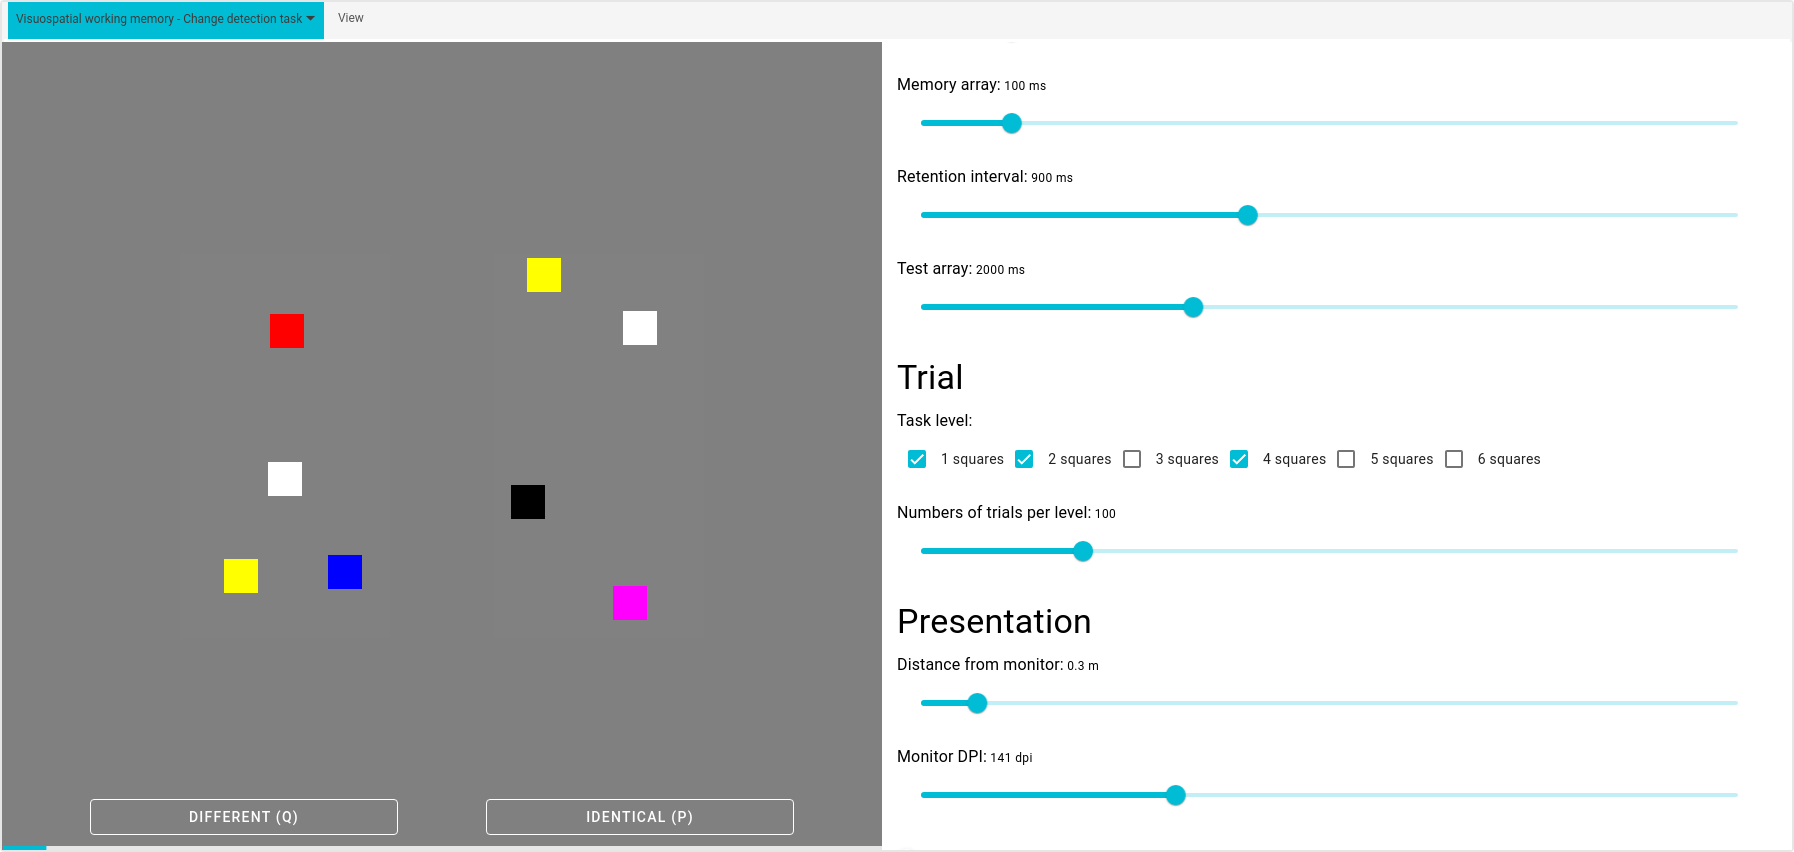
\includegraphics[width=1\textwidth]{Appendix/databases/Figures/vwm-delivery.png}
\par\end{centering}
\caption{\gls*{VWM} stimuli delivery interface.}
\label{}
\end{figure}


%======================================================================
\section{Neurofeedback} \label{appendix:neurofeedback}

Neurofeedback is attracting renewed interest as a method to self-regulate one’s own brain activity to directly alter the underlying neural mechanisms of cognition and behavior. It not only promises new avenues as a method for cognitive enhancement in healthy subjects, but also as a therapeutic tool. In the current article, we present a review tutorial discussing key aspects relevant to the development of EEG neurofeedback studies. In addition, the putative mechanisms underlying neurofeedback learning are considered. We highlight both aspects relevant for the practical application of neurofeedback as well as rather theoretical considerations related to the development of new generation protocols. Important characteristics regarding the set-up of a neurofeedback protocol are outlined in a step-by-step way. All these practical and theoretical considerations are illustrated based on a protocol and results of a frontal-midline theta up-regulation training for the improvement of executive functions. Not least, assessment criteria for the validation of neurofeedback studies as well as general guidelines for the evaluation of training efficacy are discussed \cite{enriquez2017eeg}.

\begin{figure}[H]
\begin{centering}
% \includesvg[width=0.8\textwidth]{Cap4/Figures/transformer.svg}
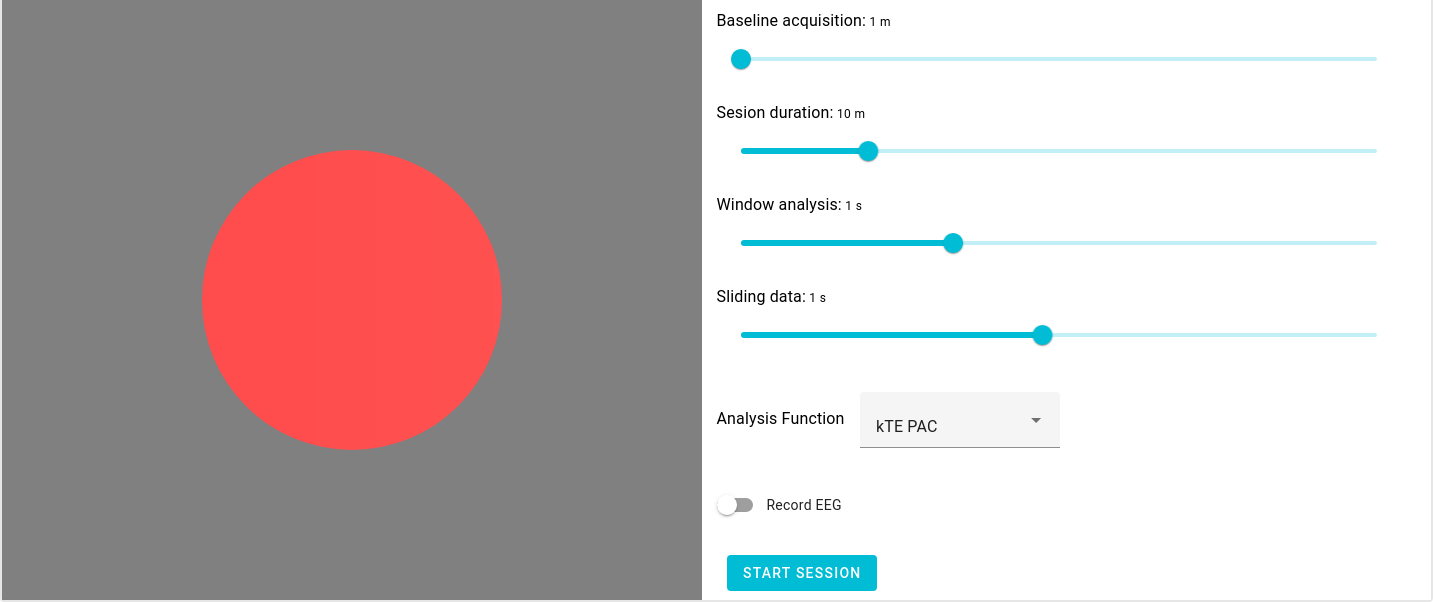
\includegraphics[width=1\textwidth]{Appendix/databases/Figures/vwm-neurofeedback.png}
\par\end{centering}
\caption{\gls*{VWM} neurofeedback dash board.}
\label{}
\end{figure}
        \chapter{Paradigm: Reward stop signal task (RSST)}\label{appendix:rsst}

The concept of inhibitory control in human cognition can be approached from its basic motor and reflexive aspects to elaborate control processes such as planned actions and strategies \cite{aron2003stop}, it can also be simply defined as the resistance to interference \cite{dempster1992rise}. From a cognitive perspective, inhibitory control is not only a fundamental tool to guide behaviour towards goals accomplishment but to dynamically modify or cancel planned actions \cite{bari2013inhibition}. This dynamic dimension of (inhibitory) cognitive control is crucial to enable the flexibility of cognitive and behavioural control systems \cite{ide2013bayesian}.

%======================================================================
\section{Paradigm}

The general principle of Stop Tasks is a routine motor reaction where participants must hit a key each time they are confronted with a frequent go stimulus, and a cancellation of the ongoing action, after exposure to an infrequent stop signal. Our visual stimuli and experimental design consist on a modified version of the SST developed by Rubia and colleagues (2003) \cite{rubia2003right}, which is, in turn, a faster visual variant of the Tracking SST \cite{logan1984ability}. Main modifications reside on the introduction of monetary feedback after each successful inhibition and the suppression of punishment feedback after a failed inhibition \cite{herrera2019expectation}.

Participants performed the Reward Stop Signal Task Paradigm (RSST) in two different groups. One group was aware of the possibility of rewards magnitudes shift but the order of rewards was not communicated (\textit{expected specific rewards group}). In the other group (\textit{unexpected reward group}), participants only knew that a monetary reward will appear without any mention to the reward shift and subsequently discovered (by themselves) a distinct reward magnitude only at the last block.


%======================================================================
\section{Stimuli presentation} 

The RSST was presented over 4 blocks of 4 min each. Each block has one of the three possible feedbacks: non-monetary reward (Smiley), low reward (50 COP) or high reward (500 COP). Regardless of the assigned condition or group, all participants performed exactly the same first – baseline- block, were each successful inhibition was rewarded with a Smiley. Afterwards, participants received two types of the mentioned monetary feedbacks.

To control for the effect of reward order presentation, we have built two conditions: for Increasing condition the order was Smiley, 50 COP, 50 COP, 500 COP; and for Decreasing condition, Smiley, 500 COP, 500 COP, 50 COP. Participants were randomly assigned to each condition in a counterbalanced way. Half of participants underwent the Increasing Condition and the other half, the Decreasing Condition.

\begin{figure}[H]
\begin{centering}
% \includesvg[width=0.8\textwidth]{Cap4/Figures/transformer.svg}
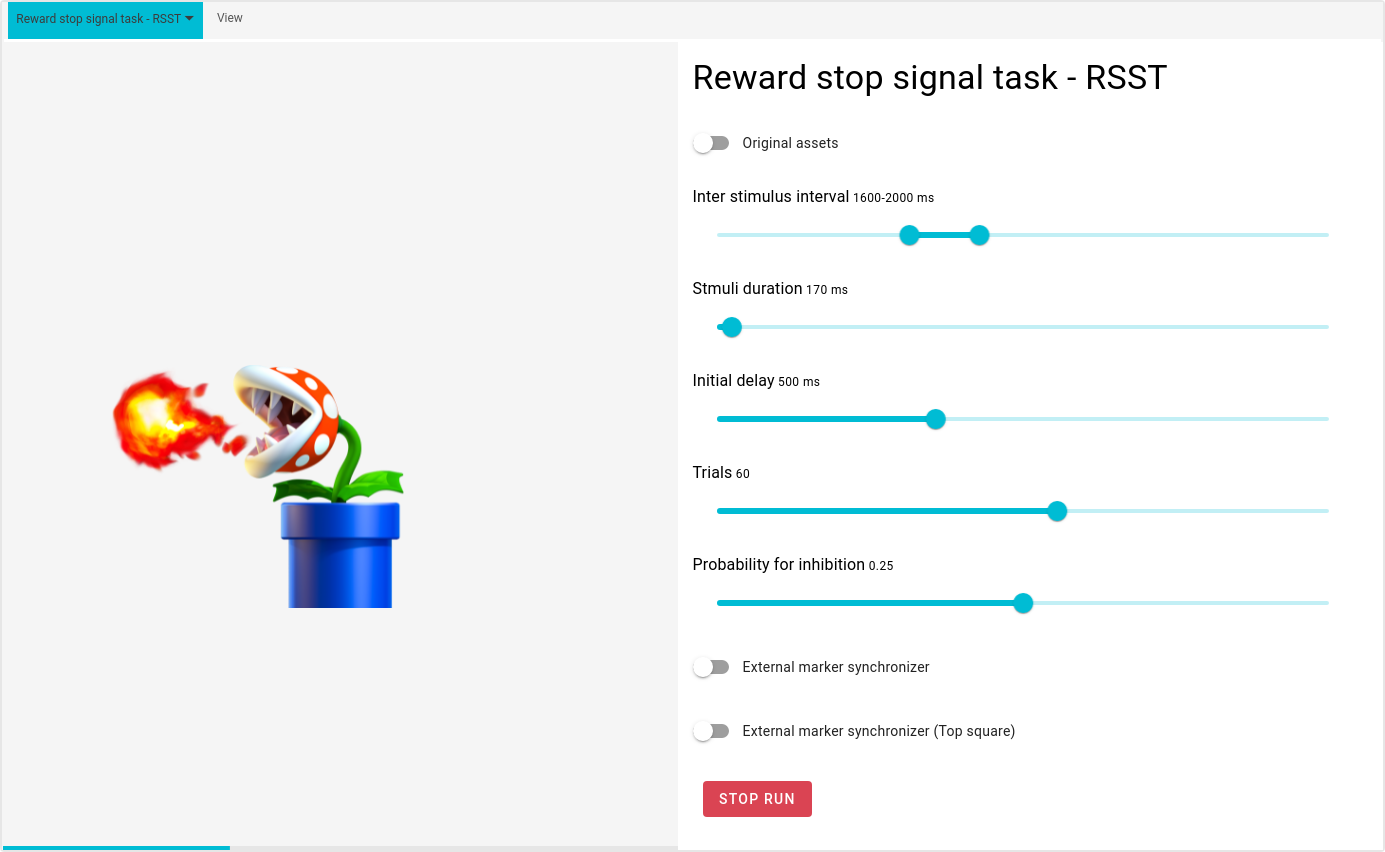
\includegraphics[width=1\textwidth]{Appendix/paradigms/Figures/rsst-delivery.png}
\par\end{centering}
\caption{\gls*{RSST} stimuli delivery dashboard.}
\label{}
\end{figure}
        % \chapter{Band modulation based neurofeedback}\label{appendix:band}

The power band modulation is one of the most common neurofeedback paradigm \cite{jones2020infant, forsyth2018comparison, gruber2002modulation},  

\begin{figure}[H]
\begin{centering}
% \includesvg[width=0.8\textwidth]{Cap4/Figures/transformer.svg}
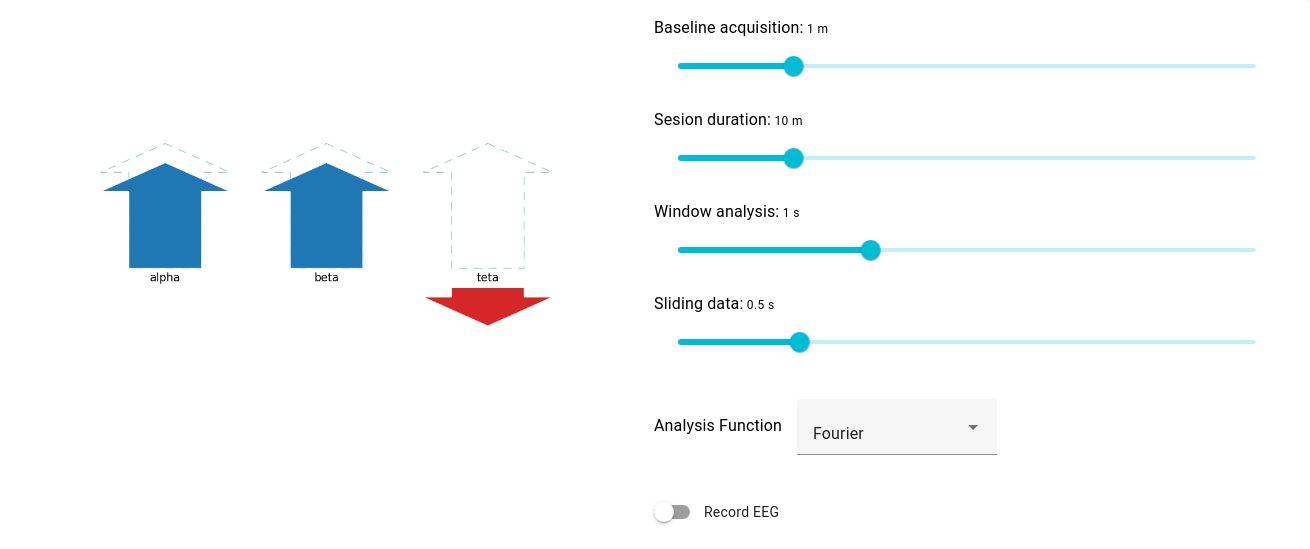
\includegraphics[width=1\textwidth]{Appendix/paradigms/Figures/band-neurofeedback.png}
\par\end{centering}
\caption{Band modulation based neurofeedback.}
\label{}
\end{figure}
    \end{appendices}
    
    % Bibliography
    \addcontentsline{toc}{chapter}{Bibliography}
    \bibliographystyle{ieeetr}
    \bibliography{References}

\end{document}